\documentclass[a5paper, twoside, 11pt, listof=nochaptergap, bahasa] {book}

%-----------------------------------------------
% packages.tex
% Package loading must be set here to ensure
% document's order
%-----------------------------------------------


\usepackage[cache=false]{minted}

% Typesetting and hyphenation helper %
\usepackage[indonesian]{babel}

% Hyperref and Outline %
\usepackage{hyperref}

% Text coloring %
\usepackage{color}

% Math typeset and equations %
\usepackage{amsmath}
\usepackage{amssymb}
\usepackage{amsfonts}

% Every first paragraph is indented %
\usepackage{indentfirst}

% For enumeration and the sorts %
\usepackage{enumitem}

% For styling titles and the sorts %
\usepackage{titlesec}
\usepackage{titletoc}

% Table of Content needs %
\usepackage[titles]{tocloft}
\usepackage{tocbibind}

% For various "if" definitions %
\usepackage{etoolbox}

% Bibliography needs %
\usepackage[backend=bibtex,style=ieee,sorting=none]{biblatex}
\usepackage{url}

% Page margin %
\usepackage[top=2.5cm, bottom=2.5cm, left=2.5cm, right=2cm]{geometry}

% Paragraph alignment %
\usepackage{ragged2e}

% References debugging purpose: change 'final' to 'draft' to use %
\usepackage[final]{showkeys}

% Include pictures %
\usepackage{graphicx}
\usepackage{wrapfig}

% Code formatting %
\usepackage{tocloft}
\usepackage{listings}
\usepackage[chapter]{algorithm}
% \usepackage[algochapter]{algorithm2e}
% \usepackage{algorithmicx}
\usepackage{algpseudocode}

% Captions formatting %
\usepackage[tableposition=top, justification=centering, labelsep=space]{caption}
\usepackage{chngcntr}

% For tables need %
\usepackage{tabularx}

% Background %
\usepackage{eso-pic}

% Fonts -- compile with xelatex for correct output %
\usepackage{fontspec}

% Header-footer needs %
\usepackage{fancyhdr}

% Tables need to be rotated smh %
\usepackage{lscape}

\newtheorem{theo}{Teorema}

% Quotation Mark in BibTeX
\usepackage[style=english]{csquotes}
%-------------------------------------------------------------
% utils.tex
% Generic commands which may be used throughout the document
% should be set here
%-------------------------------------------------------------

%--
%	A set of command for appendix testing tables
%--
\newcommand {\testtableheader}
{
	\hline
	No & \multicolumn{3}{|c|}{BSGS}           & \multicolumn{3}{c|}{Brent} \\
	& \multicolumn{1}{|l}{R} & S & Verdict & R & S & Verdict 		   \\
	\hline
}

\newcommand {\testtablefooter}
{
	\hline
}

\newenvironment{testtable}
{
	\begin{tabular}{|l|l l l|l l l|}
	\testtableheader
}
{
	\testtablefooter
	\end{tabular}
}

%--
%	Shortcut command for QED symbol. Use it while in math environment
%--
\newcommand{\eop}{\ensuremath{\blacksquare}}

% Bugs in LaTeX are damn AMAZING %
%--
%	Preventing \addvspace to throw error due to unended paragraph
%	#1: Usual parameter entered
%--
\let\oldaddvspace\addvspace
\renewcommand\addvspace[1]
{
	\par\oldaddvspace{#1}
}

%--
%	Preventing \contentsline to throw error due to unended paragraph
%	#1, #2, #3: Usual parameter entered
%--
\let\oldcontentsline\contentsline
\renewcommand\contentsline[3]
{
	\par\oldcontentsline{#1}{#2}{#3}
}

%--
%	Creates a text to denote an empty page
%--
\newcommand\emptypage
{
	\begin{center}
		[\textit{Halaman ini sengaja dikosongkan}]
	\end{center}
	\newpage
}

%--
%	Works as if applying two \clearpage, plus some text denoting
%	the page is empty
%--
\makeatletter
\def\cleardoublepage
{
	\clearpage
	\if@twoside
		\ifodd\c@page
			% do nothing
		\else
			\emptypage
		\fi
	\fi
}
\makeatother
%---------------------------------------------------------%
%--					Labelling Utilities					--%
%---------------------------------------------------------%

%----------- 1 Document hierarchies

%--
%	Auto label chapter with proper prefix
%	Param
%	#1: Label name. If not given, #2 will be used
%	#2:	The shown name
%--
\makeatletter

\let\oldchapter\chapter

\newcommand{\chapterstar}[1]
{
	\oldchapter*{#1}
	\protect\label{sec:#1}
}

\newcommand{\chapternostar}[2][]
{
	\ifstrempty{#1}
		{\oldchapter{#2}\protect\label{sec:#2}}
		{\oldchapter[#1]{#2}\protect\label{sec:#1}}
}
\renewcommand{\chapter}{\@ifstar{\chapterstar}{\chapternostar}}

\makeatother

%--
%	Auto label section with proper prefix
%	Param
%	#1: Label name. If not given, #2 will be used
%	#2:	The shown name
%--
\let\oldsection\section
\renewcommand\section[2][]
{
	\protect\oldsection{#2}
	\ifstrempty{#1}{\protect\label{sec:#2}}{\protect\label{sec:#1}}
}

%--
%	Auto label subsection with proper prefix
%	Param
%	#1: Label name. If not given, #2 will be used
%	#2:	The shown name
%--
\let\oldsubsection\subsection
\renewcommand\subsection[2][]
{
	\protect\oldsubsection{#2}
	\ifstrempty{#1}{\protect\label{sec:#2}}{\protect\label{sec:#1}}
}

%--
%	Auto label subsubsection with proper prefix
%	Param
%	#1: Label name. If not given, #2 will be used
%	#2:	The shown name
%--
\let\oldsubsubsection\subsubsection
\renewcommand\subsubsection[2][]
{
	\protect\oldsubsubsection{#2}
	\ifstrempty{#1}{\protect\label{sec:#2}}{\protect\label{sec:#1}}
}

%--
%	Auto label paragraph with proper prefix
%	Param
%	#1: Label name. If not given, #2 will be used
%	#2:	The shown name
%--
\let\oldparagraph\paragraph
\renewcommand\paragraph[2][]
{
	\protect\oldparagraph{#2}
	\ifstrempty{#1}{\protect\label{sec:#2}}{\protect\label{sec:#1}}
}

%----------- 2 Environment

%--
%	Environment for code listings. Used for proper labelling
%	Param
%	#1: Additional key-value pair
%	#2:	Caption name
%	#3: Label name, automatically prefixed
%--
\lstnewenvironment{code}[3][]
{
	\lstset{
		caption=#2,
		label=code:#3,
		#1
	}
}{}
%----------------------------------------------------
% styles.tex
% Things which alter how the document would look
% but not necessarily to be implemented is to be set here
%----------------------------------------------------

%--		Listing		--%
\lstdefinestyle{generic}
{
	basicstyle=\ttfamily\footnotesize,
	tabsize=2,
	numbers=left,
	numbersep=0.6em,			% distance between number and code
	numberstyle=\footnotesize\ttfamily\itshape,
	numberfirstline=false,
	xleftmargin=2.2em,		% starting margin exclusively for the code
	frame=single,			% frame type
	framexleftmargin=2.3em,	% distance between left frame to the element in the listing}
	framerule=1pt,
	breaklines=true,
	breakatwhitespace=true,
	breakindent=20pt,
	captionpos=b,
	escapechar=~
}

%--		Header-footer		--%
\fancypagestyle{normal}
{
	\fancyhf{}	% Remove all setting
	\fancyhead[LE,RO] {\thepage}
	\renewcommand {\headrulewidth}{0pt}
	\renewcommand {\footrulewidth}{0pt}
}
%------------------------------------------
% variables.tex
% All key-value pair should be set here
%------------------------------------------

% Variables declaration %
\def \judul {Implementasi Reduksi Poligon Menggunakan Algoritma Melkman Convex Hull yang dimodifikasi dengan Studi Kasus Sphere Online Judge 5637 LL and ErBao}
\def \penulis {Michael Julian Albertus}
\def \oj {Sphere Online Judge}
\def \soal {LL and ErBao}
\def \nomorsoal {5637}
\def \nrp {05111640000097}
\def \jurusan {Departemen Informatika}
\def \fakultas {Fakultas Teknologi Informasi dan Komunikasi}
\def \pembimbingsatu {Rully Soelaiman, S.Kom., M.Kom.}
\def \nikpembimbingsatu {19700213199402100}
\def \pembimbingdua {Yudhi Purwananto, S.Kom., M.Kom.}
\def \nikpembimbingdua {197007141997031002}

\def \juduleng {Implementation of Polygon Reduction Using Modified Melkman Convex Hull Algorithm with Case Study Sphere Online Judge 5637 LL and ErBao}
\def \jurusaneng {Informatics Department}
\def \fakultaseng {Faculty of Information Technology and Communication}

\def \CG{\textit{computational geometry }}
\def \CH{\textit{convex hull }}
\def \RCH{\textit{relative convex hull }}
\def \GS{\textit{Graham's Scan }}
\def \PT{\textit{polygon triangulation }}
\def \MC{\textit{monotone chain }}
\def \lokasi{Surabaya}
\def \tanggal{6 November 2019}
%---------------------------------------------------------
% setting.tex
% Everything that covers about the document setting
% and must be in preamble is to be implemented right here
%---------------------------------------------------------

%--		Whole document margin		--%
\setlength {\parindent}{2.5em}
\setlength {\parskip} {0.2em}

\setlist[enumerate] {itemsep=0pt, topsep=6pt, partopsep=0pt, parsep=0pt}

%--		Redactions		--%
\captionsetup[table] {skip=6pt, name={Tabel }}
\captionsetup[figure] {skip=6pt,name={Gambar }}
\captionsetup[algorithm]{labelsep=colon}

% Babel is weird
\addto\captionsindonesian
{
	\renewcommand {\lstlistingname}{Kode Sumber}
	\renewcommand {\chaptername}{BAB}
	\renewcommand {\contentsname}{DAFTAR ISI}
	\renewcommand {\listfigurename}{DAFTAR GAMBAR}
	\renewcommand {\listtablename}{DAFTAR TABEL}
	\renewcommand {\listalgorithmname}{DAFTAR PSEUDOCODE}
	\renewcommand {\lstlistlistingname}{DAFTAR KODE SUMBER}
}

%--		Document hierarchy depth		--%
\setcounter{secnumdepth}{5}

%--		Document fonts		--%
\setmainfont{Times New Roman}
\setmonofont{Courier New}


\ExplSyntaxOn
\NewDocumentCommand{\fakesc}{ o m }
 {
  \guido_fakesc:n { #2 }
  \IfNoValueTF{#1}
   {
    \tl_use:N \l__guido_temp_tl
   }
   {
    \cs_set_eq:NN #1 \l__guido_temp_tl
   }
 }
\cs_new_protected:Npn \guido_fakesc:n #1
 {
  \tl_set:Nn \l__guido_text_tl { #1 }
  \tl_replace_all:Nnn \l__guido_text_tl { ~ } { \q_space }
  \tl_set:Nn \l__guido_temp_tl { \group_begin: \footnotesize }
  \tl_map_inline:Nn \l__guido_text_tl
   {
    \token_if_eq_meaning:NNTF ##1 \q_space
     {
      \tl_put_right:Nn \l__guido_temp_tl { ~ }
     }
     {
      \int_compare:nTF { \char_value_uccode:n { `##1 } = `##1 }
       {
        \tl_put_right:Nn \l__guido_temp_tl { {\normalsize ##1} }
       }
       {
        \tl_put_right:Nn \l__guido_temp_tl { \tl_upper_case:n { ##1 } }
       }
     }
   }
  \tl_put_right:Nn \l__guido_temp_tl { \group_end: }
 }
\quark_new:N \q_space
\tl_new:N \l__guido_text_tl
\tl_new:N \l__guido_temp_tl
\ExplSyntaxOff

%--		Set the \chapter		--%
\titleformat {\chapter}				% section
[display]							% shape
{\Centering\bfseries}				% format
{\chaptername \ \Roman{chapter}}	% label
{0.4ex}								% label-section separator
{}									% before code
[]									% after 

% for unknown reason, spacing should be set using the following format
\titlespacing*{\chapter}{0pt}{-20pt}{20pt}

%--		Set the \chapter*		--%
\titleformat {name=\chapter,numberless}	% section
[display]					% shape
{\Centering\bfseries}		% format
{}							% label
{0.4ex}						% label-section separator
{}							% before code
[]							% after

%--		Set the \section		--%
\titleformat {\section}
[hang]
{\bfseries}
{\thesection }
{0ex}
{}
[\vspace{-0.9em}]

%--		Set the \subsection		--%
\titleformat {\subsection}
[hang]
{\bfseries}
{\thesubsection }
{0ex}
{}
[\vspace{-0.6em}]

%--		Set the \subsubsection		--%
\titleformat {\subsubsection}
[hang]
{\bfseries}
{\thesubsubsection }
{0ex}
{}
[\vspace{-0.6em}]

%--		Listing		--%
\lstset{style=generic}
\makeatletter
\def\lst@PlaceNumber{\ifnum\value{lstnumber}=0\else
	\llap{\normalfont\lst@numberstyle{\thelstnumber}\kern\lst@numbersep}\fi}
\makeatother

%--     Algorithmm      --%
\makeatletter
\begingroup
  \let\newcounter\@gobble
  \let\setcounter\@gobbletwo
  \globaldefs\@ne
  \let\c@loadepth\@ne
  \newlistof{algorithms}{loa}{\listalgorithmname}
\endgroup
\let\l@algorithm\l@algorithms
\makeatother

\makeatletter
\begingroup
  \let\newcounter\@gobble
  \let\setcounter\@gobbletwo
  \globaldefs\@ne 
  \let\c@loldepth\@ne
  \newlistof{listings}{lol}{\lstlistlistingname}
\endgroup
\let\l@lstlisting\l@listings
\makeatother
\renewcommand{\lstlistoflistings}{\listoflistings}

%--		Bibliography		--%
\defbibheading {bibliography}[DAFTAR PUSTAKA]{\chapter{#1}}
\urlstyle{rm}

%--		Table of Content	--%
\setlength\cftparskip{-2pt}
\setlength\cftbeforechapskip{0pt}
\setlength{\lineskip}{0pt}

% Chapter uses roman numeral
\renewcommand{\cftchapleader}{\cftdotfill{\cftdotsep}}
\newcommand{\Romannumeral}[1]{\uppercase\expandafter{\romannumeral#1}}
\renewcommand{\cftchappresnum}{\chaptername \ \Romannumeral}

% Prefix each segment
\renewcommand{\cfttabpresnum}{Tabel }
\renewcommand{\cfttabaftersnum}{}
\renewcommand{\cftfigpresnum}{Gambar }
\renewcommand{\cftfigaftersnum}{}
\renewcommand{\cftalgorithmspresnum}{Pseudocode }
\renewcommand{\cftalgorithmsaftersnum}{}
\renewcommand{\cftlistingspresnum}{Kode Sumber }
\renewcommand{\cftlistingsaftersnum}{}


% Set each segment's indentation such that none will overlap
\cftsetindents{chapter}{0em}{4.4em}
\cftsetindents{section}{2em}{2em}
\cftsetindents{figure}{0em}{6em}
\cftsetindents{table}{0em}{5em}
\cftsetindents{algorithms}{1.5em}{7em}
% \cftsetindents{listings}{1.5em}{7em}
\setlength{\cftlistingsnumwidth}{3cm}

% Algorithmic to rename require/ensure to input/output: 
\floatname{algorithm}{Pseudocode}
\renewcommand{\algorithmicrequire}{\textbf{Input:}}
\renewcommand{\algorithmicensure}{\textbf{Output:}}
% \algnewcommand\textproc{\textsc}

% Modulo 
\newcommand{\Mod}[1]{\ (\mathrm{mod}\ #1)}
\renewcommand{\mod}[1]{\ \mathrm{mod}\ #1}

% Bib
\renewcommand*{\newunitpunct}{,\space}

% Algorithm
\captionsetup[algorithm]{labelsep=space}
\lstset{ 
  deletekeywords={...}, 
  keywordstyle=\bfseries,
  language=c++,
  otherkeywords={*,vector,function,pair},
}
%---------------------------------------------------------
%	List of how words in Indonesian should be hyphenated
%---------------------------------------------------------

% Mathematic specific
\hyphenation{fak-to-ri-al}
\hyphenation{kom-bi-na-to-rik}
\hyphenation{kong-ru-en-si}
\hyphenation{mo-du-lo}
\hyphenation{mo-du-lus}
\hyphenation{mo-du-lar}
\hyphenation{per-mu-ta-si}
\hyphenation{per-ka-li-an}
\hyphenation{mul-ti-pli-ca-tive}
\hyphenation{or-der}
\hyphenation{lo-ga-rit-ma dis-kret}
\hyphenation{ex-po-nent}
\hyphenation{in-vers}
\hyphenation{te-o-re-ma}
\hyphenation{lo-ga-rit-mik}
\hyphenation{lo-ga-rith-mic}
\hyphenation{pro-por-si}
\hyphenation{fak-to-ri-sa-si}
\hyphenation{kar-di-na-li-tas}
\hyphenation{po-li-no-mi-al}
\hyphenation{po-ly-no-mi-al}	
\hyphenation{stan-dar de-vi-a-si}

\hyphenation{pol-lard rho}
\hyphenation{ba-by step gi-ant step}
\hyphenation{euler to-tient func-ti-on}
\hyphenation{mul-ti-point eval-u-a-tion}

% Problem specific
\hyphenation {dsa at-tack}
\hyphenation {sig-na-tu-re}
\hyphenation {run-ti-me}
\hyphenation {krip-to-gra-fi}
\hyphenation {re-pe-at-ed squ-a-ring}
\hyphenation {ge-ne-ra-tor}
\hyphenation {pu-blic}
\hyphenation {pri-va-te}
\hyphenation {key}
\hyphenation {pri-mi-ti-ve root}
\hyphenation {bru-te for-ce}
\hyphenation {ran-dom func-ti-on}
\hyphenation {step}
\hyphenation {in-te-ger o-ver-flow}
\hyphenation {mul-ti-pli-ca-ti-on}
\hyphenation {ex-po-nent-i-a-ti-on}
\hyphenation {pri-ma-li-ty}
\hyphenation {strong li-ar}
\hyphenation {pro-ba-bi-lis-tik}
\hyphenation {de-ter-mi-nis-tik}
\hyphenation {struct}
\hyphenation {po-int-er}

% Miscellaneous
\hyphenation {meng-ha-sil-kan}
\hyphenation {a-kan}
\hyphenation {ber-ja-lan}
\hyphenation {di-de-fi-ni-si-kan}
\hyphenation {bi-sa}

% Departement
\hyphenation{fa-kul-tas tek-no-lo-gi in-for-ma-si dan ko-mu-ni-ka-si}
\hyphenation{fa-cul-ty of in-for-ma-ti-on tech-no-lo-gy and com-mu-ni-ca-ti-on}	
\addbibresource{bib/source.bib}

\begin{document}
\begin{sloppypar}
	% \algnewcommand\textproc{}
	% \algnewcommand\textproc{\textsc}
	%-- Things that should go first but can't be placed in preamble
	% Figure numbering uses chapter numbering as prefix
	\counterwithin {figure}{chapter}
	
	\pagestyle {normal}
	%--
	
	\frontmatter
		\newpage
	\newgeometry{top=7cm,left=2cm,bottom=2cm}

	\sffamily
	\thispagestyle{empty}
	\color{white}
	{ \noindent TUGAS AKHIR - IF184802 }\\*[10pt] 
	{\large\textbf{\MakeUppercase{\judul}}} \\*[32pt]
	\\
	\\
	\\
	\MakeUppercase{\penulis} \\*
	NRP \nrp \\*[10pt]
	Dosen Pembimbing 1 \\*
	\pembimbingsatu \\*[10pt]
	Dosen Pembimbing 2 \\*
	\pembimbingdua \\*[10pt]
	\MakeUppercase{\jurusan} \\*
	\fakultas \\*
	Institut Teknologi Sepuluh Nopember \\*
	Surabaya, 2020
	\AddToShipoutPictureBG*{
\includegraphics[width=\paperwidth,height=\paperheight]{pembuka/img/sampul.png}}
	\rmfamily
	\normalsize
	\restoregeometry
	\color{black}
	\cleardoublepage
	
\newpage
	\newgeometry{top=7cm,left=2cm,bottom=2cm}

	\sffamily
	\thispagestyle{empty}
	{ \noindent TUGAS AKHIR - IF184802 }\\*[10pt] 
	{\large\textbf{\MakeUppercase{\judul}}} \\*[32pt]
	\\
	\\
	\\
	\MakeUppercase{\penulis} \\*
	NRP \nrp \\*[10pt]
	Dosen Pembimbing 1 \\*
	\pembimbingsatu \\*[10pt]
	Dosen Pembimbing 2 \\*
	\pembimbingdua \\*[10pt]
	\MakeUppercase{\jurusan} \\*
	\fakultas \\*
	Institut Teknologi Sepuluh Nopember \\*
	Surabaya, 2020
	\AddToShipoutPictureBG*{
\includegraphics[width=\paperwidth,height=\paperheight]{pembuka/img/sampulWhite.png}}
	\rmfamily
	\normalsize
	\restoregeometry
	\color{black}
	\cleardoublepage

\newpage
	\newgeometry{top=7cm,left=2cm,bottom=2cm}
	\sffamily
	\thispagestyle{empty}
	{\noindent UNDERGRADUATE THESES - IF184802 } \\*[10pt]
	{\large\textbf{\MakeUppercase{\juduleng}}} \\*[32pt]
	\\
	\\
	\\
	\\
	\MakeUppercase{\penulis} \\*
	NRP \nrp \\*[10pt]
	Supervisor 1 \\*
	\pembimbingsatu \\*[10pt]
	Supervisor 2 \\*
	\pembimbingdua \\*[10pt]
	\MakeUppercase{\jurusaneng} \\*
	\fakultaseng \\*
	Institut Teknologi Sepuluh Nopember \\*
	Surabaya, 2020
	\AddToShipoutPictureBG*{
\includegraphics[width=\paperwidth,height=\paperheight]{pembuka/img/sampulWhite.png}}
	\rmfamily
	\normalsize
	\restoregeometry
	\color{black}
	\cleardoublepage

		\chapter{LEMBAR PENGESAHAN}
\small

\begin{center}
	\textbf{\MakeUppercase\judul}
	\vspace*{0.3em}
	
	\textbf{TUGAS AKHIR} \\
	Diajukan Guna Memenuhi Salah Satu Syarat\\
	Memperoleh Gelar Sarjana Komputer\\
	pada\\
	Bidang Studi Algoritma Pemrograman\\
	Program Studi S-1 \jurusan\\
	\fakultas \\
	Institut Teknologi Sepuluh Nopember
	
	\vspace*{0.3em}
	
	Oleh:\\
	\textbf{\penulis} \\
	NRP. \nrp
	
	\vspace*{1.1em}
\end{center}

Disetujui oleh Dosen Pembimbing Tugas Akhir: \\
\vspace*{1.3em}

\begin{tabularx}{\linewidth}{ @{}l r }
	\pembimbingsatu & ........................... \vspace*{1.4em} \\
	NIP. \nikpembimbingsatu & (Pembimbing 1) \vspace*{2.6em} \\
	
	\pembimbingdua & ........................... \vspace*{1.4em} \\
	NIP. \nikpembimbingdua & (Pembimbing 2) \vspace*{0.9em}
\end{tabularx}

\begin{center}
	\textbf {\lokasi} \\
	\textbf {\tanggal}
\end{center}

\normalsize
\cleardoublepage
		\chapter {ABSTRAK}

% ---- Indonesian vers.

\noindent\textbf{\MakeUppercase\judul}
\vspace*{1em}

\begin{tabularx}{\linewidth}{ l l p{2.2in} }
	Nama 			& : & \penulis \\
	NRP 			& :	& \nrp \\
	Departemen 		& : & \jurusan, \newline \fakultas, ITS \\
	Pembimbing I 	& : & \pembimbingsatu \\
	Pembimbing II 	& : & \pembimbingdua
	\vspace*{1em} 	% HACKY--USE ALTERNATIVE IF POSSIBLE %
\end {tabularx}

\noindent\textbf{Abstrak} \\
\itshape
\textit{Computational geometry} adalah cabang dari ilmu komputer yang dikhususkan untuk mempelajari algoritma yang dapat dinyatakan dalam suatu geometri. Salah satu algoritma yang sering dipakai pada \CG adalah algoritma \CH. \textit{Convex hull} adalah sebuah set polygon dari titik pada bidang \textit{euclidean} atau ruang \textit{euclidean}, atau dapat disebut himpunan cembung terkecil yang berisi titik. Convex hull dapat divisualisasikan sebagai bentuk yang tertutup oleh karet gelang yang membentang di sekitar titik - titik tersebut.\\\\
\textit{Relative convex hull} merupakan penurunan dari \textit{convex hull}. \textit{Relative convex hull} merupakan \textit{convex hull} yang mempunyai \textit{cavity} (cekungan ke dalam) yang diakibatkan atau relatif terhadap sesuatu yang membatasi \textit{convex hull} tersebut. \\\\
Topik Tugas Akhir ini mengulas algoritma reduksi poligon untuk menyelesaikan permasalahan \textit{relative convex hull}. Melalui pengujian dan studi kasus didapatkan bahwa algoritma reduksi poligon dapat menyelesaikan permasalahan \textit{relative convex hull} dengan efisien.

\vspace*{1em}
\noindent\bfseries Kata Kunci: geometri; convex hull; algoritma reduksi poligon; relative convex hull;
\normalfont
\cleardoublepage

% ---- English vers.
\chapter {ABSTRACT}
\noindent\textbf{\MakeUppercase\juduleng}
\vspace*{1em}

\begin{tabularx}{\linewidth}{ l l p{2.2in} }
	Name 			& : & \penulis \\
	Student ID		& :	& \nrp \\
	Department 		& : & \jurusaneng, \newline \fakultaseng, ITS \\
	Supervisor I 	& : & \pembimbingsatu \\
	Supervisor II 	& : & \pembimbingdua
	\vspace*{1em} 	% HACKY--USE ALTERNATIVE IF POSSIBLE %
\end {tabularx}
	
\noindent\textbf{Abstract} \\
\itshape
computational geometry is one of the computer science branches that mainly focus in studying geometrical algorithm. One of the algorithm that mostly used is convex hull. Convex hull is a polygon from multiple point inside of euclidean plane. In short, minimum convex polygon that covers set of points. convex hull can be visualized by a rubber band that covers the set of points.\\\\
Relative convex hull derived from convex hull. Relative convex hull is convex hull that have one or more cavity that relative to some thing that limit the convex polygon.\\\\
In this Thesis will review polygon reduction algorithm to solve relative convex hull problem. According to sub-sequence testing and case study, it appears that polygon reduction algorithm can solve relative convex hull problem efficiently.

\vspace*{1em}
\noindent\bfseries Keywords: geometry; convex hull; polygon reduction algorithm; relative convex hull;
\normalfont
\cleardoublepage
		\chapter {KATA PENGANTAR}

Puji syukur penulis panjatkan kepada Tuhan Yang Maha Esa. Atas rahmat dan kasih sayangNya, penulis dapat menyelesaikan tugas akhir dan laporan akhir dalam bentuk buku ini.

Pengerjaan buku ini penulis tujukan untuk mengeksplorasi lebih mendalam topik-topik yang tidak diwadahi oleh kampus, namun banyak menarik perhatian penulis. Selain itu besar harapan penulis bahwa pengerjaan tugas akhir sekaligus pengerjaan buku ini dapat menjadi batu loncatan penulis dalam menimba ilmu yang bermanfaat.

Penulis ingin menyampaikan rasa terima kasih kepada banyak pihak yang telah membimbing, menemani dan membantu penulis selama masa pengerjaan tugas akhir maupun masa studi.

\begin {enumerate}
	\item Bapak Rully Soelaiman S.Kom.,M.Kom., selaku pembimbing penulis. Ucapan terima kasih juga penulis sampaikan atas segala perhatian, didikan, pengajaran, dan nasihat yang telah diberikan oleh beliau selama masa studi penulis.
\end {enumerate}

Penulis menyadari bahwa buku ini jauh dari kata sempurna. Maka dari itu, penulis memohon maaf apabila terdapat salah kata maupun makna pada buku ini. Akhir kata, penulis mempersembahkan buku ini sebagai wujud nyata kontribusi penulis dalam ilmu pengetahuan.

\begin{flushright}
Surabaya, 5 November 2019
\vspace{5em}
\penulis
\end{flushright}
		\tableofcontents\cleardoublepage
\listoffigures\cleardoublepage
\listoftables\cleardoublepage

\addcontentsline{toc}{chapter}{\listalgorithmname}
\listofalgorithms\cleardoublepage

\addcontentsline{toc}{chapter}{\listoflistingscaption}
\lstlistoflistings

		\chapter{DAFTAR NOTASI}
\begin{tabularx}{\linewidth}{c X}
	$ \sum $ & Notasi yang digunakan untuk menjumlahkan sejumlah bilangan terurut dengan aturan tertentu. \\
	$ \forall $ & Notasi yang mewakili setiap element pada himpunan\\
	$ \left \langle ...\right \rangle$ & Notasi untuk menyatakan himpunan\\
	$ \left | ...  \right |$ & Notasi untuk menyatakan banyak anggota himpunan\\
\end{tabularx}
	
	\mainmatter
		\vspace{0ex}
\chapter {PENDAHULUAN}

Pada bab ini, akan dijelaskan mengenai latar belakang, rumusan masalah, batasan masalah, tujuan, metodologi pengerjaan, dan sistematika penulisan Tugas Akhir.

\section{Latar Belakang}

\par \textit{Computational geometry} adalah cabang dari ilmu komputer yang dikhususkan untuk mempelajari algoritma yang dapat dinyatakan dalam suatu geometri. Salah satu algoritma yang sering dipakai pada \CG adalah algoritma \CH. \textit{Convex hull} adalah sebuah set polygon dari titik pada bidang \textit{euclidean} atau ruang \textit{euclidean}, atau dapat disebut himpunan cembung terkecil yang berisi titik. Sebagai contoh, ketika suatu kumpulan titik merupakan bagian yang dibatasi dalam sebuah bidang, \CH dapat divisualisasikan sebagai bentuk yang tertutup oleh karet gelang yang membentang di sekitar titik - titik tersebut. Berikut merupakan contoh dari \CH :
\begin{figure}[!h]
	\Centering
	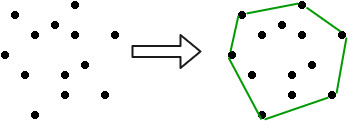
\includegraphics [width=\textwidth]{bab1/img/ilustrasi-convex-hull}
	\caption {Ilustrasi Convex Hull}
	\label {fig:ilustrasi-convex-hull}
\end{figure}
\par \textit{Relative convex hull} merupakan penurunan dari \textit{convex hull}. \textit{Relative convex hull} merupakan \textit{convex hull} yang mempunyai \textit{cavity} (cekungan ke dalam) yang diakibatkan atau relatif terhadap sesuatu yang membatasi \textit{convex hull} tersebut. Ilustrasi \textit{relative convex hull} dapat dilihat pada gambar \ref{fig:ilustrasi-relative-convex-hull}.

\begin{figure}[!h]
	\Centering
	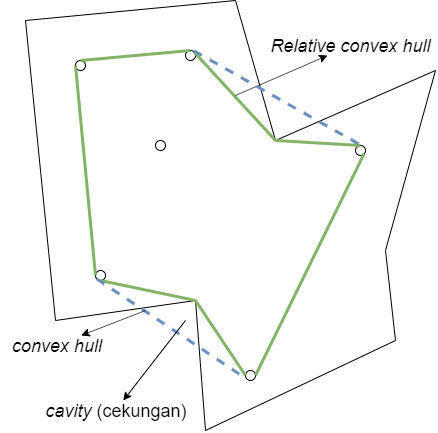
\includegraphics [width=0.5\columnwidth]{bab2/img/ilustrasi-relative-convex-hull}
	\caption {Ilustrasi Relative Convex Hull}
	\label {fig:ilustrasi-relative-convex-hull}
\end{figure}

\par Pada topik Tugas Akhir ini akan dijelaskan algoritma penyelesaian untuk mencari \textit{relative convex hull} dari sekumpulan titik yang berada di dalam sebuah polygon sederhana dengan menggunakan reduksi polygon pada studi kasus pada Sphere Online Judge 5637 LL and ErBao.

\section {Rumusan Masalah}

Rumusan masalah yang diangkat dalam Tugas Akhir ini adalah sebagai berikut :

\begin {enumerate}
    \item Bagaimana mencari \RCH dari kumpulan titik di dalam sebuah polygon?
    \item Bagaimana reduksi polygon menyelesaikan masalah \RCH dari kumpulan titik?
\end {enumerate}

\section {Batasan Masalah}
\label{sec:batasan_masalah}
Permasalahan yang dibahas pada Tugas Akhir ini memiliki beberapa batasan, yaitu sebagai berikut :
\begin{enumerate}
    \item Implementasi reduksi polygon sebagai penyelesaian permasalahan \RCH pada soal ISUN1.
    \item Algoritma \RCH terbatas pada analisis intuitif yang logis.
\end{enumerate}
Berikut merupakan batasan pada situs Sphere Online Judge: 
\begin {enumerate}
    \item Implementasi dilakukan menggunakan bahasa pemrograman C++.
    \item Banyaknya sisi pada polygon pembatas ($n$) diantara 3 sampai 500.
    \item Banyaknya pohon yang berada dalam taman ($m$) diantara 0 sampai 500.
    \item Batas maksimum untuk tiap vertex memenuhi($ x $, $ y $) dimana nilai |$x$|, |$y$| $\leq 10000$. 
    \item Banyak soal tidak diketahui karena program berhenti sampai EOF.
    \item Batas waktu yang diberikan adalah $ 0.142 $ detik.
    \item Batas memori yang diberikan adalah $ 1.536 $ MB.
    \item Batas kode sumber yang diberikan adalah $ 50.000 $ B. 
\end {enumerate}

\section {Tujuan}
Tujuan Tugas Akhir ini adalah sebagai berikut :
\begin{enumerate}
    \item Mengevaluasi kinerja reduksi polygon untuk menyelesaikan permasalahan komputasi \textit{relative convex hull} pada LL and ErBao.
\end{enumerate}

\section {Manfaat}
Tugas Akhir ini mampu memberikan pemahaman algoritma yang tepat untuk menyelesaikan permasalahan komputasi \textit{relative convex hull} dengan efisien.

\section {Metodologi}
Metodologi pengerjaan yang digunakan pada Tugas Akhir ini memiliki beberapa tahapan. Tahapan-tahapan tersebut yaitu :

\begin{enumerate}
    \item Penyusunan proposal\\
    Pada tahapan ini penulis memberikan penjelasan mengenai apa yang penulis akan lakukan dan mengapa Tugas Akhir ini dilakukan. Penjelasan tersebut dituliskan dalam bentuk proposal Tugas Akhir.
    \item Studi literatur\\
    Pada tahapan ini penulis mengumpulkan referensi yang diperlukan guna mendukung pengerjaan Tugas Akhir. Referensi yang digunakan dapat berupa hasil penelitian yang sudah pernah dilakukan, buku, artikel internet, atau sumber lain yang bisa dipertanggungjawabkan.
    \item Implementasi algoritma\\
    Pada tahapan ini penulis mulai mengembangkan algoritma yang digunakan untuk menyelesaikan permasalahan komputasi \textit{relative convex hull}.
    \item Pengujian dan evaluasi\\
    Pada tahapan ini penulis menguji performa algoritma yang digunakan. Hasil pengujian kemudian dievaluasi untuk kemudian dipertimbangkan apakah algoritma masih bisa ditingkatkan lagi atau tidak.
    \item Penyusunan buku\\
    Pada tahapan ini penulis menyusun hasil pengerjaan Tugas Akhir mengikuti format penulisan Tugas Akhir.
\end{enumerate}

\section {Sistematika Penulisan}
Sistematika laporan Tugas Akhir yang akan digunakan adalah sebagai berikut :
\begin{enumerate}
    \item BAB I : PENDAHULUAN\\
    Bab ini berisi latar belakang, rumusan masalah, batasan masalah, tujuan, manfaat, metodologi dan sistematika penulisan Tugas Akhir.
    \item BAB II : DASAR TEORI\\
    Bab ini berisi dasar teori mengenai permasalahan dan algoritma penyelesaian yang digunakan dalam Tugas Akhir
    \item BAB III : DESAIN\\
    Bab ini berisi desain algoritma dan struktur data yang digunakan dalam penyelesaian permasalahan.
    \item BAB IV : IMPLEMENTASI\\
    Bab ini berisi implementasi berdasarkan desain algoritma yang telah dilakukan pada tahap desain.
    \item BAB V : UJI COBA DAN EVALUASI\\
    Bab ini berisi uji coba dan evaluasi dari hasil implementasi yang telah dilakukan pada tahap implementasi.
    \item BAB VI : PENUTUP\\
    Bab ini berisi kesimpulan dan saran yang didapat dari hasil uji coba yang telah dilakukan.
\end{enumerate} \cleardoublepage
		\chapter {DASAR TEORI}

Pada bab ini, akan dijelaskan dasar teori yang digunakan sebagai landasaan pengerjaan Tugas Akhir ini.

\section{Deskripsi Permasalahan}
Permasalahan yang dibahas pada Tugas Akhir ini adalah perhitungan untuk mencari nilai $x$ yang didefinisikan oleh persamaan \eqref{eq:perimeter-polygon}.
\begin{equation}
    \label{eq:perimeter-polygon}
    x=\sum_{i=0}^{n-1} \text{RCH}_i
\end{equation}
$\text{RCH}_i$ pada persamaan \eqref{eq:perimeter-polygon} menyatakan sisi polygon dari RCH yang merupakan \textit{relative convex hull} yang didapatkan dari sekumpulan titik yang dibatasi di dalam polygon sederhana\cite{isun1}. Permasalahan pada tugas akhir ini adalah mencari \textit{relative convex hull} dari sekumpulan titik yang dibatasi oleh polygon sederhana. Gambar \ref{fig:ilustrasi-contoh-kasus-tanpa-solusi} dan \ref{fig:ilustrasi-contoh-kasus} merupakan contoh dari permasalahan ISUN1.
\begin{figure}
	\Centering
	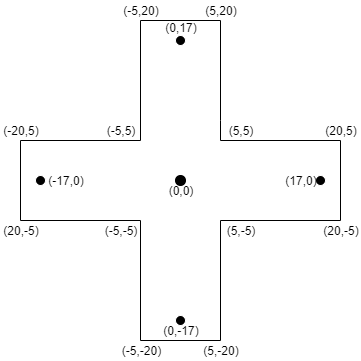
\includegraphics [width=0.5\columnwidth]{bab2/img/contoh-kasus-tanpa-solusi}
	\caption {Ilustrasi contoh kasus tanpa solusi}
	\label {fig:ilustrasi-contoh-kasus-tanpa-solusi}
\end{figure}
\begin{figure}
	\Centering
	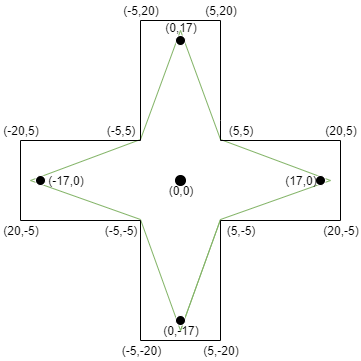
\includegraphics [width=0.5\columnwidth]{bab2/img/contoh-kasus}
	\caption {Ilustrasi contoh kasus}
	\label {fig:ilustrasi-contoh-kasus}
\end{figure}

\section{Convex Polygon}
Merupakan sebuah polygon sederhana yang memiliki sudut maksimal 180 derajat pada tiap edgenya. \textit{Convex polygon} memiliki beberapa properti, yaitu:
\begin{enumerate}
    \item sebuah garis lurus yang di gambar melewati sebuah \textit{convex} polygon akan berpotongan maksimal 2 kali. Ilustrasi dapat dilihan pada gambar \ref{fig:ilustrasi-properti-convex-polygon-1}
    \item Jika dua titik sembarang diambil dan ditarik garis antara keduanya, tidak ada bagian dari garis yang berada di luar polygon. Ilustrasi dapat dilihan pada gambar \ref{fig:ilustrasi-properti-convex-polygon-2}
\end{enumerate}
\begin{figure}
    \Centering
    
\includegraphics[width=0.5\columnwidth]{bab2/img/ilustrasi-properti-convex-polygon-1}
    \caption{Ilustrasi Properti Convex Polygon 1}
    \label{fig:ilustrasi-properti-convex-polygon-1}
\end{figure}
\begin{figure}
    \Centering
    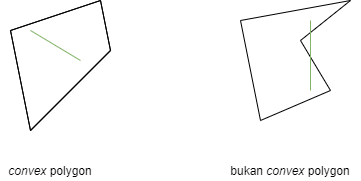
\includegraphics[width=0.5\columnwidth]{bab2/img/ilustrasi-properti-convex-polygon-2}
    \caption{Ilustrasi Properti Convex Polygon 2}
    \label{fig:ilustrasi-properti-convex-polygon-2}
\end{figure}

\subsection{Relative Convex Polygon}
Merupakan penurunan dari convex Polygon tetapi ada beberapa sisi dari polygon tersebut berbentuk convace atau cekung kedalam dikarenakan adanya batasan dari luar seperti polygon atau segmen garis lainnya. Ilustrasi relative convex polygon dapat dilihat pada gambar \ref{fig:ilustrasi-relative-convex-polygon}.
\begin{figure}
    \Centering
    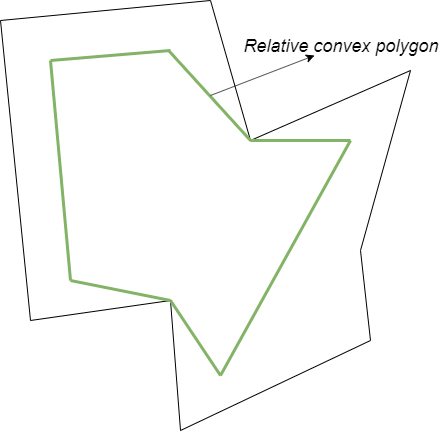
\includegraphics[width=0.5\columnwidth]{bab2/img/ilustrasi-relative-convex-polygon}
    \caption{Ilustrasi Relative Convex Polygon}
    \label{fig:ilustrasi-relative-convex-polygon}
\end{figure}
\section{Strategi Penyelesaian Permasalahan}
Pada subbab ini akan dipaparkan mengenai strategi penyelesaian masalah klasik pada daring SPOJ dengan kode ISUN1 menggunakan algoritma reduksi poligon. Secara singkat, strategi penyelesaian masalah dari ISUN1 menggunakan algoritma reduksin poligon menjadi 2 bagian besar yaitu :
\begin{enumerate}
    \item Pemrosesan titik pembentuk polygon yang membentuk \textit{Convex}.
    \item \textit{Convex Hull} dari titik yang berada didalam polygon
\end{enumerate}
Sebagai contoh, pada subbab ini akan menggunakan $P$ sebagai poligon luar yang mempunyai $n$ vertex, dimana $P = \left \langle p_1, p_2, ..., p_n \right \rangle$ yang mempunyai titik sebanyak $m$ ($S = \left \langle s_1, s_2, ..., s_m \right \rangle$), dan $D(A)$ merupakan sebuah deque (\textit{doubly-ended queue}) yang menampung vertex dari polygon $P$. Reduksi polygon didasari dari algoritma Melkman dengan sedikit modifikasi. Modifikasi yang dilakukan adalah ketika 3 buak titik pembentuk poligon yang konsekutif membuat \textit{convex} maka titik tengan dari ketiga titik tersebut dibuang, dan jika \textit{concave} maka titik tengahnya tetap disimpan. Pada saat sebuah titik dibuang, maka luas dari polygon akan tereduksi. Langkah - langkah reduksi dilakukan dengan mengulangi 2 langkah yang akan dijelaskan pada subbab \ref{sec:pemrosesan-titik-pembentuk-polygon-yang-membentuk-convex} dan \ref{sec:convex-hull-dari-titik-yang-berada-di-dalam-polygon}


\subsection{Pemrosesan Titik Pembentuk Polygon yang Membentuk Convex}
\label{sec:pemrosesan-titik-pembentuk-polygon-yang-membentuk-convex}
Pemrosesan titik pembentuk poligon dapat dilakukan dengan cara melakukan \textit{traversing} terhadap semua vertex pembentuk poligon. Untuk setiap vertex $p_i$ yang di cek, hitung orientasi(secara berlawanan jarum jam) titik $p_i$ dengan $p_{i-1}$ dan $ p_{i+1}$. Jika orientasinya membentuk \textit{convex} maka titik $p_i$ akan dibuang.
\par Sebelum membuang titik $p_i$, kita akan membuat sebuah segitiga $ABC$ dimana $A=p_i$, $B=p_{i-1}$, dan $C=p_{i+1}$ karena triangulation of polygon(Teorema \ref{theo:triangulation-of-polygon}).
\begin{theo}[Triangulation of Polygon]
    \label{theo:triangulation-of-polygon}
	Semua polygon dapat di buat dari beberapa segitiga.
\end{theo}
Kemudian cari $T(ABC)$ dimana $T(ABC)$ merupakan semua titik $S$ yang berada di dalam segitiga $ABC$ dengan menggunakan algoritma \textit{Point inside Polygon} (dapat dilihat pada subbab \ref{sec:point-inside-polygon}). Pencarian titik yang berada di dalam segitiga $ABC$ berguna untuk mencari pengganti vertex $p_i$ sebagai pembentuk poligon luarnya.

\subsection{Convex Hull dari Titik yang Berada di Dalam Polygon}
\label{sec:convex-hull-dari-titik-yang-berada-di-dalam-polygon}
Melanjutkan dari subbab \ref{sec:pemrosesan-titik-pembentuk-polygon-yang-membentuk-convex}, ketika sudah mendapatkan $T$, lakukan pencarian \textit{Convex Hull} dari titik - titik tersebut menggunakan \textit{monotone chain} (dapat dilihat pada subbab \ref{sec:algoritma-monotone-chain}). Kemudian sisipkan semua titik yang membentuk \textit{Convex Hull} diantara vertex $p_{i-1}$, $p_{i+1}$ untuk me-rekonstruksi poligon luar yang sudah di reduksi.

\section{Convex Hull}
\label{sec:convex-hull}
\textit{Convex Hull} dari sekumpulan titik $S$ adalah sebuah set dari semua kombinasi \textit{convex} dari titik - titik tersebut. Setiap titik $s_i$ pada $S$ diberikan sebuah koefisien $a_i$ dimana $a_i$ merupakan bialangan non negatif dan jika semua $a_i$ dijumlahkan hasilnya satu. Dan koefisien ini digunakan untuk menghitung berat rata - rata untuk setiap titik. Untuk setiap koefisien yang dipilih akan dikombinasikan dan menghasilkan \textit{convex hull}. Set \textit{convex hull} ini dapat di ekspresikan dengan formula \eqref{eq:convex-hull} dan ilustrasi \textit{convex hull} ada pada gambar \ref{fig:ilustrasi-convex-hull}.

\begin{equation}
    \label{eq:convex-hull}
    Conv(S)=\left\{ \sum_{i=1}^{|S|}{a_is_i} \big | (\forall{i}:a_i \ge 0 \wedge \sum_{i=1}^{|S|}{a_i=1} ) \right\}
\end{equation}
\begin{figure}
	\Centering
	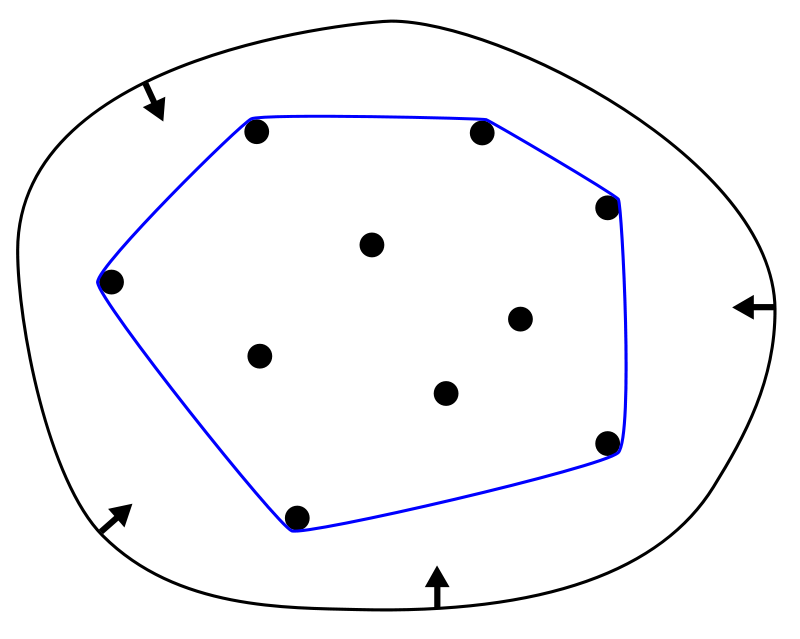
\includegraphics [width=0.5\columnwidth]{bab2/img/ilustrasi-convex-hull}
	\caption {Ilustrasi Convex Cull}
	\label {fig:ilustrasi-convex-hull}
\end{figure}


\subsection{Relative Convex Hull}
\textit{Relative convex hull} merupakan penurunan dari \textit{convex hull}. \textit{Relative convex hull} merupakan \textit{convex hull} yang mempunyai \textit{cavity} (cekungan kedalam) yang diakibatkan atau relatif terhadap sesuatu yang membatasi \textit{convex hull tersebut}. ilustrasi \textit{relative convex hull} dapat dilihat pada gambar \ref{fig:ilustrasi-relative-convex-hull}.

\begin{figure}
	\Centering
	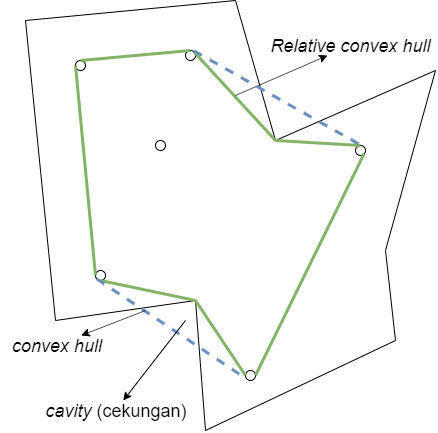
\includegraphics [width=0.5\columnwidth]{bab2/img/ilustrasi-relative-convex-hull}
	\caption {Ilustrasi Relative Convex Hull}
	\label {fig:ilustrasi-relative-convex-hull}
\end{figure}
\par Penentuan untuk mengetahui sebuah polygon merupakan \textit{convex} atau \textit{concave} dapat menggunakan orientasi. Apabila orientasi dari tiga titik yang berurutan adalah positif berlawanan jarum jam maka tiga titik tersebut adalah \textit{convex}. Sebaliknya apabila negatif maka tiga titik tersebut adalah \textit{concave}. Untuk mencari orientasi antara tiga titik dapat digunakan persamaan \ref{eq:orientasi}.
\begin{equation}
    \begin{aligned}
    \label{eq:orientasi}
        \vec{u}&=(B_x-A_x)x +(B_y-A_y)y\\
        \vec{v}&=(C_x-A_x)x +(C_y-A_y)y\\
    \end{aligned}
\end{equation}
$$ Orientasi = u_x*v_y - u_y*v_x $$
\subsection{Algoritma Convex Hull}
Ada beberapa algoritma yang dapat digunakan untuk mencari sebuah \textit{convex hull}, untuk melihat perbandingan dari beberapa algoritma dapat dilihat pada tabel \ref{tab:tabel-algoritma-convex-hull}.
\begin{table}[]
    \Centering
    \newcolumntype{P}[1]{>{\centering\arraybackslash}p{#1}}
    \caption{Tabel Perbandingan Algoritma Convex Hull}
    \label{tab:tabel-algoritma-convex-hull}
    \begin{tabular}{|P{2cm}|P{2cm}|P{2cm}|P{1.5cm}|P{2cm}|}
        \hline
    Algoritma Convex Hull & Implementasi & Kompleksitas & Kode Sumber     & Jenis Input \\ \hline
    Jarvis's Algorithm    & Mudah                  & $\mathcal{O}(n^2)$         & Singkat         & Kumpulan Titik\\ \hline
    Graham's Scan         & Sedikit Mudah          & $\mathcal{O}(n\log(n))$  & Singkat         & Kumpulan Titik  \\ \hline
    Quick Hull            & Kompleks               & $\mathcal{O}(n\log(n))$  & Panjang         & Kumpulan Titik  \\ \hline
    Monotone Chain        & Mudah                  & $\mathcal{O}(n\log(n))$  & Singkat         & Kumpulan Titik  \\ \hline
    Melkman's Algorithm   & Mudah                  & $\mathcal{O}(n)$           & Singkat         & Poligon Sederhana \\ \hline    
    \end{tabular}
\end{table}
Berdasarkan tabel \ref{tab:tabel-algoritma-convex-hull}, penulis memilih 2 algoritma yang akan digunakan pada buku ini.
\subsubsection{Algoritma Melkman Convex Hull}
\label{sec:algoritma-melkman-convex-hull}
Merupakan algoritma untuk menghitung rantai polygonal ataupun polygon sederhana dengan waktu linear $\mathcal{O}(n)$\cite{melkman_algorithm}. Asumsikan sebuah poligon sederhana $P$, dengan vertex $p_i$ dan edge $p_i p_{i+1}$. Algoritma ini menggunakan deque, $D = \left \langle d_1, d_2, ..., d_n \right \rangle$, untuk mereprentasikan \CH, $Q_i = CH(P_i)$, dimana $P_i = (p_0, p_1, ..., p_i)$. Deque mempunyai fungsi \textit{push} dan \textit{pop} dari atas/depan dan \textit{insert} dan \textit{remove} dari bawah/belakang. Secara spesifiknya yang dilakukan \textit{push} $v$ ke deque melakukan $(l \leftarrow l+1; d_t \leftarrow v)$, untuk \textit{pop} $d_t$ dari deque melakukan $(t \leftarrow t-1)$, untuk insert $v$ ke deque melakukan $(b \leftarrow b-1; d_b \leftarrow v)$, dan \textit{remove} $d_b$ dari deque melakukan $(b \leftarrow b+1)$.
\par Algoritma ini menggunakan konvensi dimana vertexnya berurutan secara berlawanan jarum jam di sekitar \CH $Q$.
\par Setiap $d_t$ dan $d_b$ mengacu kepada vertex yang sama pada rantai polygon $C$, dan vertex ini akan selalu menjadi vertex yang kita tambahkan terakhir pada \CH. Pseudocode Melkman Convex Hull dapat dilihat pada pseudocode \ref{psdo:Melkman-Convex-Hull}.
\begin{figure}
	\Centering
	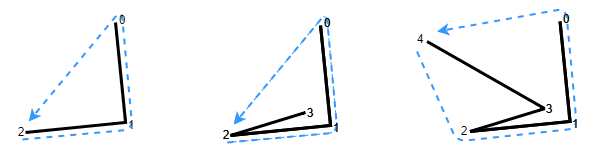
\includegraphics [width=\columnwidth]{bab2/img/ilustrasi-algoritma-melkman}
	\caption {Ilustrasi Algoritma Melkman}
	\label {fig:ilustrasi-algoritma-melkman}
\end{figure}
\begin{algorithm}
	\caption{Melkman Convex Hull}
	\label{psdo:Melkman-Convex-Hull}
	\begin{algorithmic}[1]
		\Require $P$
		\Ensure $Q$
        \State Inisialisasi: $D$
        \If{\fakesc{Left}($p_0, p_1, p_2$)}
            \State$D \leftarrow \left \langle p_2, p_0, p_1, p_2 \right \rangle$
        \Else
            \State $D \leftarrow \left \langle p_2, p_1, p_0, p_2 \right \rangle$
        \EndIf
        \State $i=3$
        \While{$i<n$}
            \While{ \fakesc{Left}($d_{t-1}, d_t, p_i$) dan \fakesc{Left}($d_b, d_{b+1}, p_i$))} 
                \State $i \leftarrow i+1$
            \EndWhile
            \While{!\fakesc{Left}($d_{t-1}, d_t, p_i$)}
                \State \textit{pop} $d_t$
            \EndWhile
            \State \textit{push} $p_i$
            \While{!\fakesc{Left}($p_i,d_{b}, d_{b+1}$)}
                \State \textit{remove} $d_b$
            \EndWhile
            \State \textit{insert} $p_i$
            \State $i \leftarrow i+1$
        \EndWhile
	\end{algorithmic}
\end{algorithm}

\subsubsection{Algoritma Monotone Chain}
\label{sec:algoritma-monotone-chain}
Algoritma \MC merupakan proses pembentukan \CH dari sekumpulan titik dengan kompleksitas $\mathcal{O}(n$ log$(n))$\cite{monotone_chain_algorithm}. Asumsikan sekumpulan titik $S$ sejumlah $n$ ,$S = \left \langle s_1, s_2, ..., s_n\right \rangle$ algoritma ini menggunakan list untuk membentuk sebuah rantai (\textit{monotone chain}), dimana list $L(S)$ menampung semua titik yang ada di $S$ yang terurut berdasarkan nilai koordinatnya terhadap sumbu $x$. algoritma ini memeriksa setiap 3 vertex yang berurutan, jika 3 vertex tersebut membuat \textit{convex} makan ketiga vertex tersebut disimpan, dan sebaliknya jika ketiga vertex tersebut membuat \textit{concave} maka vertex ke 2 akan dibuang dari vertex penyusun \textit{convex hull}. lalu lakukan hal yang sama dengan membalikan urutan pada $L$ untuk mendapatkan \textit{lower hull}. Pseudocode algoritma \textit{Monotone Chain} dapat dilihat pada pseudocode \ref{psdo:Monotone-Chain-Algorithm}.

\begin{figure}
	\Centering
	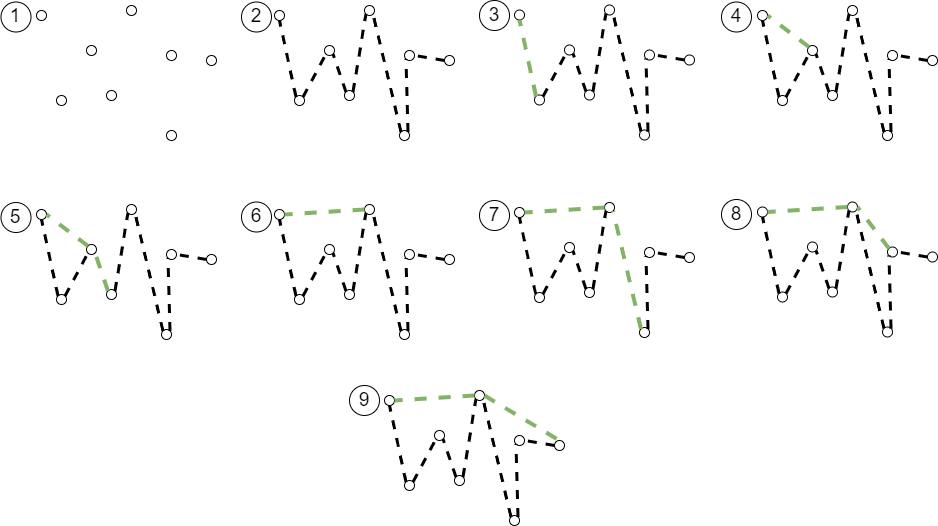
\includegraphics [width=\columnwidth]{bab2/img/ilustrasi-algoritma-monotone-chain}
	\caption {Ilustrasi Algoritma Monotone Chain}
	\label {fig:ilustrasi-algoritma-monotone-chain}
\end{figure}

\begin{algorithm}
	\caption{Monotone Chain Algorithm}
	\label{psdo:Monotone-Chain-Algorithm}
	\begin{algorithmic}[1]
		\Require $S$
		\Ensure $CH(S)$
        \State Inisialisasi: $L$
        \State Sort $S$
        \State $L \leftarrow S$
        \State Inisialisasi $CH(S)$
        \For{$i=0;i<2;i++$}
            \For{$j=0;j<Size(L);j++$}
                \While{$Size (CH)\ge2$ and $right(CH[Size(CH)-1],CH[Size(CH)-2],S[j])$}
                    \State Delete $CH$ last element
                \EndWhile
                \State push $pt$ to $CH$
            \EndFor
            \State reverse $L$
        \EndFor
	\end{algorithmic}
\end{algorithm}
\section{Point Inside Polygon}
\label{sec:point-inside-polygon}
\textit{Point Inside Polygon} merupakan algoritma untuk menentukan apakah suatu polygon berada di dalam sebuah polygon atau tidak \cite{point_inside_polygon}. Ide utama dari algoritma ini adalah dengan cara menarik garis sejajar dengan sumbu $x$ dimana garis tersebut berujung pada titik yang ingin dicari lokasinya kemudian hitung ada berapa edge dari poligon yang berpotongan dengan garis tersebut. Jika jumlah edge polygon yang berpotongan adalah ganjil, maka titik tersebut berada dalam polygon, dan sebaliknya, jika jumlahnya genap maka titik tersebut berada di luar polygon.

\begin{figure}
	\Centering
	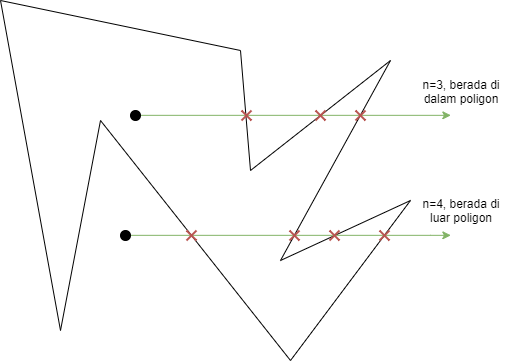
\includegraphics [width=0.5\columnwidth]{bab2/img/ilustrasi-algoritma-point-inside-polygon}
	\caption {Ilustrasi Algoritma Point Inside Polygon}
	\label {fig:ilustrasi-algoritma-point-inside-polygon}
\end{figure}
 \cleardoublepage
		\chapter{DESAIN}
\label{sec:desain}
Pada bab ini akan dijelaskan desain algoritma yang akan digunakan untuk menyelesaikan permasalahan.

\section{ Desain Umum Sistem}
\label{sec:desain-umum-sistem}
Pada subbab ini akan dijelaskan mengenai gambaran secara umum dari algoritma yang dirancang. Sistem diawali dengan menerima masukan 2 buah bilangan bulat $N$ yang merupakan banyaknya vertex pembentuk polygon luar dan $M$ yang merupakan banyaknya titik yang ada di dalam polygon tersebut. $N$ baris berikutnya berisikan 2 buah bilangan bulat $x_i$, $y_i$ yang merupakan koordinat dari vertex pembentuk polygon luar terurut berlawanan arah jarum jam. $M$ baris berikutnya berisikan dua buah bilangan bulat $x1_i$, $y1_i$ yang merupakan koordinat dari titik yang ada di dalam polygon.

\subsection{ Desain Fungsi Main}
Fungsi \fakesc{main} merupakan fungsi yang bertanggung jawab untuk menerima masukan yang sudah dijelaskan pada \ref{sec:desain-umum-sistem} untuk dilakukan proses selanjutnya. Pseudocode fungsi \fakesc{main} dapat dilihat pada pseudocode \ref{psdo:fungsi-main}. Fungsi \fakesc{Input} merupakan fungsi untuk menerima masukan, dan fungsi \fakesc{Print} merupakan fungsi untuk menampilkan hasil. 

\begin{algorithm}
	\caption{Fungsi \fakesc{main}}
	\label{psdo:fungsi-main}
    \begin{algorithmic}[1]
        \While{($N \leftarrow $ \fakesc{Input()}) and $N \neq EOF$}
            \State $M \leftarrow$ \fakesc{Input()}
            \State $perimeter \leftarrow$ \fakesc{Polygon}
            \State $trees \leftarrow$ Array \fakesc{Point}   
            \For {$i \leftarrow 1, N$}
                \State $x_i , y_i \leftarrow $ \fakesc{Input()}
                \State $perimeter.P[i]\leftarrow$ \fakesc{Point}($x_i$, $y_i$, false)
			\EndFor
			\If{$M=1$ or $M=0$}
				\State \fakesc{Print}($0$)
				\State \fakesc{Continue}
			\EndIf
            \For {$i \leftarrow 1, M$}
                \State $ x1_i , y1_i \leftarrow $ \fakesc{Input()}
                \State $trees \leftarrow$ \fakesc{Point}($x1_i$, $y1_i$, true)
            \EndFor
            \State $ans \leftarrow $\fakesc{Solve}($perimeter$, $trees$)
            \State \fakesc{Print} ($ans $)
        \EndWhile
	\end{algorithmic}
\end{algorithm}
\subsection{ Desain Class Point}
\label{sec:point}
Class \fakesc{Point} adalah class untuk menyimpan titik dalam diagram Kartesius. Pseudocode \ref{psdo:class-point} merupakan pseudocode dari class \fakesc{Point}. Nantinya pada implementasi, class ini akan melakukan \textit{override} terhadap operator perbandingan.
\begin{table}[htb]
	\Centering
	\caption{Nama dan Fungsi Variabel dalam Class \fakesc{Point}}
	\begin{tabular}{|c|p{7cm}|}
	\hline
	Nama Variabel & \multicolumn{1}{c|}{Fungsi Variabel}                               \\ \hline
$x$           & Menyimpan ordinat dari titik tersebut  \\ \hline
$y$           & Menyimpan absis dari titik tersebut          \\ \hline
$fixed$             & Untuk membedakan antara titik pembentuk polygon $P$ dan titik yang ada di dalam kumpulan titik $S$   \\ \hline
	\end{tabular}
	\label{tab:var-point}
\end{table}
\begin{algorithm}
	\caption{Class \fakesc{Point}}
	\label{psdo:class-point}
	\begin{algorithmic}[1]
        \State $ x, y \leftarrow $ \textbf{double}
        \State $fixed \leftarrow $ \textbf{boolean}
		\State \textbf{constructor} \Call{\fakesc{Point}}{$ $}
        \State \textbf{constructor} \Call{\fakesc{Point}}{$ \_x, \_y, \_fixed $}
	\end{algorithmic}
\end{algorithm}

Class \fakesc{Point} tidak memiliki fungsi karena class ini memang hanya untuk menyimpan suatu titik yang akan digunakan nanti.

Fungsi \textit{Constructor} dari class ini terdiri dari dua jenis. Fungsi \textit{constructor} yang pertama adalah fungsi dengan tanpa parameter, pada \textit{constructor} ini, semua variabel yang ada di dalam class \fakesc{Point} akan di inisialisasi dengan $0$. Fungsi \textit{constructor} kedua adalah fungsi dengan parameter $\_x, \_y, \_fixed$, menyatakan nilai $x, y, fixed$ secara berurutan.

\subsection{ Desain Class Vec}
\label{sec:vec}
Class \fakesc{Vec} merupakan class yang menyimpan vector dari dua buah titik pada diagram kartesian. Pseudocode \ref{psdo:class-vec} merupakan pseudocode dari class \fakesc{Vec}. 

\begin{table}[htb]
	\Centering
	\caption{Nama dan Fungsi Variabel dalam Class \fakesc{Vec}}
	\begin{tabular}{|c|p{7cm}|}
	\hline
	Nama Variabel & \multicolumn{1}{c|}{Fungsi Variabel}                               \\ \hline
$x$           & Menyimpan arah vektor absis  \\ \hline
$y$           & Menyimpan arah vektor ordinat          \\ \hline
	\end{tabular}
	\label{tab:var-vec}
\end{table}
\begin{algorithm}
	\caption{Class \fakesc{Vec}}
	\label{psdo:class-vec}
	\begin{algorithmic}[1]
        \State $ x, y \leftarrow $ \textbf{double}
		\State \textbf{constructor} \Call{\fakesc{Vec}}{$ $}
        \State \textbf{constructor} \Call{\fakesc{Vec}}{$ \_x, \_y $}
        \State \textbf{constructor} \Call{\fakesc{Vec}}{$ A, B $}
	\end{algorithmic}
\end{algorithm}

Class \fakesc{Vec} tidak memiliki fungsi karena class ini hanya untuk menyimpan vector dari dua titik yang akan digunakan nanti.

Fungsi \textit{Constructor} dari class ini terdiri dari 3 jenis. Fungsi \textit{constructor} yang pertama adalah fungsi dengan tanpa parameter, pada \textit{constructor} ini, semua variabel yang ada di dalam class \fakesc{Vec} akan di inisialisasi dengan $0$. Fungsi \textit{constructor} kedua adalah fungsi dengan parameter $\_x, \_y$, menyatakan nilai $x, y$ secara berurutan. Fungsi \textit{constructor} ketiga adalah fungsi dengan parameter $A, B$, menyatakan \fakesc{Point} dari titik $A$ dan \fakesc{Point} dari titik $B$, dimana nantinya nilai $x$ dan $y$ akan didapatkan dari pengurangan koordinat dari \fakesc{Point} $A$ dan \fakesc{Point} $B$.

\subsection{ Desain Class Line}
\label{sec:line}
Class \fakesc{Line} merupakan class yang bertanggung jawab untuk melakukan operasi-operasi pada garis dalam diagram kartesian. Pseudocode \ref{psdo:class-line} merupakan pseudocode dari Class \fakesc{Line}. 

\begin{table}[htb]
	\Centering
	\caption{Nama dan Fungsi Variabel dalam class \fakesc{Line}}
	\begin{tabular}{|c|p{7cm}|}
	\hline
	Nama Variabel & \multicolumn{1}{c|}{Fungsi Variabel}                               \\ \hline
$a$           & Menyimpan nilai $a$ pada persamaan $ax + by + c =0$ \\ \hline
$b$           & Menyimpan nilai $b$ pada persamaan $ax + by + c =0$          \\ \hline
$c$           & Menyimpan nilai $c$ pada persamaan $ax + by + c =0$          \\ \hline
	\end{tabular}
	\label{tab:var-line}
\end{table}
\begin{algorithm}
	\caption{Class \fakesc{Line}}
	\label{psdo:class-line}
	\begin{algorithmic}[1]
        \State $ a, b, c \leftarrow $ \textbf{double}
		\State \textbf{constructor} \Call{\fakesc{Line}}{$ $}
        \State \textbf{constructor} \Call{\fakesc{Line}}{$ \_a, \_b, \_c $}
        \State \textbf{constructor} \Call{\fakesc{Line}}{$ A, B $}
	\end{algorithmic}
\end{algorithm}

Class \fakesc{Line} tidak memiliki fungsi karena class ini hanya untuk menyimpan nilai dari fungsi $ax+by+c=0$ yang akan digunakan nanti.

Fungsi \textit{Constructor} dari class ini terdiri dari 3 jenis. Fungsi \textit{constructor} yang pertama adalah fungsi dengan tanpa parameter, pada \textit{constructor} ini, semua variabel yang ada di dalam class \fakesc{Line} akan di inisialisasi dengan $0$. Fungsi \textit{constructor} kedua adalah fungsi dengan parameter $\_a, \_b, \_c$, menyatakan nilai $a, b, c$ secara berurutan. Fungsi \textit{constructor} ketiga adalah fungsi dengan parameter $A, B$, menyatakan \fakesc{Point} dari titik $A$ dan \fakesc{Point} dari titik $B$, dimana nantinya nilai $a$, $b$ dan $c$ akan didapatkan dengan mencari fungsi garis yang melewati \fakesc{Point} $A$ dan \fakesc{Point} $B$.

\subsection{ Desain Class Segment}
\label{sec:segment}
Class \fakesc{Segment} merupakan class yang bertanggung jawab untuk menyimpan dan melakukan operasi-operasi pada segmen garis dalam diagram kartesian. Pseudocode \ref{psdo:class-segment} merupakan pseudocode dari class \fakesc{Segment}. 

\begin{table}[htb]
	\Centering
	\caption{Nama dan Fungsi Variabel dalam Class \fakesc{Segment}}
	\begin{tabular}{|c|p{7cm}|}
	\hline
	Nama Variabel & \multicolumn{1}{c|}{Fungsi Variabel}                               \\ \hline
$P$           & Menyimpan \fakesc{Point} yang merupakan ujung awal dari sebuah segmen garis \\ \hline
$Q$           & Menyimpan \fakesc{Point} yang merupakan ujung akhir dari sebuah segmen garis          \\ \hline
$L$           & Menyimpan fungsi dari garis yang melalui dua titik tersebut      \\ \hline
	\end{tabular}
	\label{tab:var-segment}
\end{table}
\begin{algorithm}
	\caption{Class \fakesc{Segment}}
	\label{psdo:class-segment}
	\begin{algorithmic}[1]
        \State $ P, Q \leftarrow $ \fakesc{Point}
        \State $L \leftarrow$ \fakesc{Line}
		\State \textbf{constructor} \Call{\fakesc{Segment}}{$ $}
        \State \textbf{constructor} \Call{\fakesc{Segment}}{$ \_P, \_Q$}
	\end{algorithmic}
\end{algorithm}

Class \fakesc{Segment} tidak memiliki fungsi karena class ini hanya untuk menyimpan data dari sebuah segmen garis yang akan digunakan nanti.

Fungsi \textit{Constructor} dari class ini terdiri dari 2 jenis. Fungsi \textit{constructor} yang pertama adalah fungsi dengan tanpa parameter, pada \textit{constructor} ini, semua variabel yang ada di dalam class \fakesc{Segment} akan di inisialisasi dengan $0$. Fungsi \textit{constructor} kedua adalah fungsi dengan parameter $\_P, \_Q$, menyatakan \fakesc{Point} dari titik $P$ dan \fakesc{Point} dari titik $Q$, yang merupakan titik \fakesc{Point} $A$ dan \fakesc{Point} $B$ secara berturut, dan \fakesc{Line} $L$ didapar dengan menggunakan \textit{constructor} \fakesc{Line} dengan parameter $P$ dan $Q$.

\subsection{ Desain Class Polygon}
\label{sec:polygon}
Class \fakesc{Polygon} merupakan class yang bertanggung jawab untuk menyimpan dan melakukan operasi-operasi pada polygon pada diagram kartesian. Pseudocode \ref{psdo:class-polygon} merupakan pseudocode dari class \fakesc{Polygon}. 

\begin{table}[htb]
	\Centering
	\caption{Nama dan Fungsi Variabel dalam Class \fakesc{Polygon}}
	\begin{tabular}{|c|p{7cm}|}
	\hline
	Nama Variabel & \multicolumn{1}{c|}{Fungsi Variabel}                               \\ \hline
$P$           & Menyimpan array dari \fakesc{Point} yang membentuk polygon tersebut \\ \hline
	\end{tabular}
	\label{tab:var-polygon}
\end{table}
\begin{algorithm}
	\caption{Class \fakesc{Polygon}}
	\label{psdo:class-polygon}
	\begin{algorithmic}[1]
        \State $ P \leftarrow $ Array \fakesc{Point}
		\State \textbf{constructor} \Call{\fakesc{Polygon}}{$ $}
        \State \textbf{constructor} \Call{\fakesc{Polygon}}{$ \_P$}
        \State \textbf{function} \Call{\fakesc{prev}}{$ idx $}
		\State \textbf{function} \Call{\fakesc{next}}{$ idx $}
		\State \textbf{function} \Call{\fakesc{perimeter}}{$ $}
	\end{algorithmic}
\end{algorithm}

Fungsi-fungsi yang terkandung dalam class ini adalah \fakesc{prev}, \fakesc{next}, \fakesc{perimeter}. Tabel \ref{tab:var-polygon} menjelaskan variabel dan kegunaannya dalam class \fakesc{Polygon}. 

Fungsi \textit{Constructor} dari class ini terdiri dari 2 jenis. Fungsi \textit{constructor} yang pertama adalah fungsi dengan tanpa parameter, pada \textit{constructor} ini, variabel $P$ yang ada di dalam class \fakesc{Polygon} akan di inisialisasi. Fungsi \textit{constructor} kedua adalah fungsi dengan parameter $\_P$, menyatakan array \fakesc{Point} dari titik pembentuk polygon tersebut.

Fungsi \textit{next} bertanggung jawab untuk mencari index selanjutnya dari titik yang membentuk polygon. Masukan, proses dan keluaran dari fungsi ini tercantum pada tabel \ref{tab:class-polygon-next}. Pseudocode fungsi ini dapat dilihat pada pseudocode \ref{psdo:class-polygon-next}.

\begin{table}[htb]
	\Centering
	\caption{Masukan, Proses, dan Keluaran dari Fungsi \fakesc{Next} Class \fakesc{Polygon}}
	\begin{tabular}{|p{3cm}|p{3cm}|p{3cm}|}
	\hline
	Masukan   & Proses     & Keluaran \\ \hline
	Suatu bilangan bulat $idx$ yang menyatakan index saat ini & mencari index selanjutnya &   Suatu bilangan bulat yang menyatakan index selanjutnya     \\ \hline
	\end{tabular}
	\label{tab:class-polygon-next}
\end{table}

\begin{algorithm}
    \caption{Fungsi \fakesc{Next} pada class \fakesc{Polygon}}
	\label{psdo:class-polygon-next}
	\begin{algorithmic}[1]
        \Require $ idx $
        \If{$idx = $\fakesc{Size}($P$)$-1$}
            \State \Return $0$
        \Else
            \State \Return $idx+1$
		\EndIf
	\end{algorithmic}
\end{algorithm}

Fungsi \textit{prev} bertanggung jawab untuk mencari index sebelumnya dari titik yang membentuk polygon. Masukan, proses dan keluaran dari fungsi ini tercantum pada tabel \ref{tab:class-polygon-prev}. Pseudocode fungsi ini dapat dilihat pada pseudocode \ref{psdo:class-polygon-prev}.

\begin{table}[htb]
	\Centering
	\caption{Masukan, Proses, dan Keluaran dari Fungsi \fakesc{Prev} Class \fakesc{Polygon}}
	\begin{tabular}{|p{3cm}|p{3cm}|p{3cm}|}
	\hline
	Masukan   & Proses     & Keluaran \\ \hline
	Suatu bilangan bulat $idx$ yang menyatakan index saat ini & mencari index sebelumnya &   Suatu bilangan bulat yang menyatakan index sebelumnya     \\ \hline
	\end{tabular}
	\label{tab:class-polygon-prev}
\end{table}

\begin{algorithm}
    \caption{Fungsi \fakesc{Prev} pada class \fakesc{Polygon}}
	\label{psdo:class-polygon-prev}
	\begin{algorithmic}[1]
        \Require $ idx $
        \If{$idx = 0$}
            \State \Return \fakesc{Size}($P$)$-1$
        \Else
            \State \Return $idx-1$
		\EndIf
	\end{algorithmic}
\end{algorithm}

Fungsi \textit{perimeter} bertanggung jawab untuk mencari keliling dari sebuah polygon. Masukan, proses, dan keluaran dari fungsi ini tercantum pada tabel \ref{tab:class-polygon-perimeter}. Pseudocode fungsi ini dapat dilihat pada pseudocode \ref{psdo:class-polygon-perimeter}.
\begin{table}[htb]
	\Centering
	\caption{Masukan, Proses, dan Keluaran dari Fungsi \fakesc{Perimeter} Class \fakesc{Polygon}}
	\begin{tabular}{|p{3cm}|p{3cm}|p{3cm}|}
	\hline
	Masukan   & Proses     & Keluaran \\ \hline
	- & Mencari keliling dengan mencari jarak eulerian dari semua titik pembentuk polygon &   Suatu bilangan berkoma yang menyatakan keliling dari polygon tersebut     \\ \hline
	\end{tabular}
	\label{tab:class-polygon-perimeter}
\end{table}

\begin{algorithm}
    \caption{Fungsi \fakesc{Perimeter} pada class \fakesc{Polygon}}
	\label{psdo:class-polygon-perimeter}
    \begin{algorithmic}[1]
        \State $ret \leftarrow 0$
        \For{$i \leftarrow 0$ \textbf{to} \fakesc{Size}($P$)$-1$}
            \State $ret \leftarrow ret $ \fakesc{EDist}($P[i]$, $P[$ \fakesc{next}($i$)$] $)
        \EndFor
        \State \Return $ret$
	\end{algorithmic}
\end{algorithm}

\subsection{ Desain Fungsi BetweenD}
\label{sec:fungsi-betweend}
Fungsi \fakesc{BetweenD} bertanggung jawab untuk mencari tahu apakah suatu bilangan $x$ berada diantara bilangan $l$ dan bilangan$r$. Pseudocode dari fungsi \fakesc{BetweenD} dapat dilihat pada pseudocode \ref{psdo:fungsi-betweend}. Masukan, proses, dan keluaran dari fungsi ini tercantum pada tabel \ref{tab:fungsi-betweend}.

\begin{table}[htb]
	\Centering
	\caption{Masukan, Proses, dan Keluaran dari Fungsi \fakesc{BetweenD} }
	\begin{tabular}{|p{3cm}|p{3cm}|p{3cm}|}
	\hline
	Masukan   & Proses     & Keluaran \\ \hline
	Tiga buah bilangan $x,l,r$, dimana bilangan $x$ merupakan bilangan yang ingin diketahui apakah berada diantara titik $l$ dan $r$ & Mencari tahu apakah bilangan $x$ berada diantara bilangan $l$ dan $r$ &   Sebuah boolean yang menyatakan apakah $x$ berada diantara $l$ dan $r$     \\ \hline
	\end{tabular}
	\label{tab:fungsi-betweend}
\end{table}
\begin{algorithm}
    \caption{Fungsi \fakesc{BetweenD}}
	\label{psdo:fungsi-betweend}
    \begin{algorithmic}[1]
        \Require $x, l, r$
        \If{\fakesc{Min}($l, r$) $\le x + EPS$ and $x \le$ \fakesc{Max}($l, r$) $+ EPS$}
            \State \Return \fakesc{True}
        \Else
            \State \Return \fakesc{False}
        \EndIf
	\end{algorithmic}
\end{algorithm}


\subsection{ Desain Fungsi EDist}
\label{sec:fungsi-edist}
Fungsi \fakesc{EDist} bertanggung jawab untuk mencari jarak antara dua titik \fakesc{Point} $A$ dan \fakesc{Point} $B$ dengan menggunakan rumus \textit{Pythagoras}. Rumus \textit{Pythagoras} dapat di lihat pada persamaan \ref{eq:pythagoras}. Pseudocode fungsi \fakesc{EDist} dapat dilihat pada pseudocode \ref{psdo:fungsi-edist}. Masukan, proses, dan keluaran dari fungsi ini tercantum pada tabel \ref{tab:fungsi-edist}.

\begin{equation}
    \label{eq:pythagoras}
    C=\sqrt{A^2 + B^2}
\end{equation}

\begin{table}[htb]
	\Centering
	\caption{Masukan, Proses, dan Keluaran dari Fungsi \fakesc{EDist} }
	\begin{tabular}{|p{3cm}|p{3cm}|p{3cm}|}
	\hline
	Masukan   & Proses     & Keluaran \\ \hline
	Dua buah \fakesc{Point} $A$ dan \fakesc{Point} $B$ yang akan dicari jaraknya & Mencari jarak antara \fakesc{Point} $A$ dan \fakesc{Point} $B$ &   Sebuah bilangan berkoma yang menyatakan jarak \fakesc{Point} $A$ dan \fakesc{Point} $B$  \\ \hline
	\end{tabular}
	\label{tab:fungsi-edist}
\end{table}

\begin{algorithm}
    \caption{Fungsi \fakesc{EDist}}
	\label{psdo:fungsi-edist}
    \begin{algorithmic}[1]
        \Require $A, B$
        \State \Return \fakesc{Sqrt}($(A*A)+(B*B)$)
	\end{algorithmic}
\end{algorithm}

\subsection{ Desain Fungsi Cross}
\label{sec:fungsi-cross}
Fungsi \fakesc{Cross} bertanggung jawab untuk mencari nilai perkalian \textit{cross} dari dua buah vector. Rumus Pythagoras dapat di lihat pada persamaan \ref{eq:cross}. Pseudocode fungsi \fakesc{Cross} dapat dilihat pada pseudocode \ref{psdo:fungsi-cross}. Masukan, proses, dan keluaran dari fungsi ini tercantum pada tabel \ref{tab:fungsi-cross}.

\begin{equation}
    \label{eq:cross}
    C = (u_x*v_y) - (u_y*v_x)
\end{equation}
\begin{table}[htb]
	\Centering
	\caption{Masukan, Proses, dan Keluaran dari Fungsi \fakesc{Cross} }
	\begin{tabular}{|p{3cm}|p{3cm}|p{3cm}|}
	\hline
	Masukan   & Proses     & Keluaran \\ \hline
	Dua buah \fakesc{Vec} $U$ dan \fakesc{Vec} $V$ yang akan dicari hasil perkalian silangnya & Mencari nilai perkalian silang dari \fakesc{Vec} $U$ dan \fakesc{Vec} $V$ &   Sebuah bilangan yang menyatakan hasil perkalian silang \fakesc{Vec} $U$ dan \fakesc{Vec} $V$  \\ \hline
	\end{tabular}
	\label{tab:fungsi-cross}
\end{table}


\begin{algorithm}
    \caption{Fungsi \fakesc{Cross}}
	\label{psdo:fungsi-cross}
    \begin{algorithmic}[1]
        \Require $U, V$
        \State \Return $(U.x*V.y) - (U.y*V.x)$
	\end{algorithmic}
\end{algorithm}

\subsection{ Desain Fungsi Orientation}
\label{sec:fungsi-orientation}
Fungsi \fakesc{Orientation} bertanggung jawab untuk mencari orientasi dari tiga titik. Pseudocode fungsi \fakesc{Orientation} dapat dilihat pada pseudocode \ref{psdo:fungsi-orientation}. Masukan, proses, dan keluaran dari fungsi ini tercantum pada tabel \ref{tab:fungsi-orientation}.

\begin{table}[htb]
	\Centering
	\caption{Masukan, Proses, dan Keluaran dari Fungsi \fakesc{Orientation} }
	\begin{tabular}{|p{3cm}|p{3cm}|p{3cm}|}
	\hline
	Masukan   & Proses     & Keluaran \\ \hline
	Tiga buah \fakesc{Point} $O$, \fakesc{Point} $P$ dan \fakesc{Point} $Q$ yang akan dicari orientasinya & Mencari orientasi antara \fakesc{Point} $O$, \fakesc{Point} $P$ dan \fakesc{Point} $Q$ &   Sebuah bilangan yang menyatakan orientasi antara \fakesc{Point} $O$, \fakesc{Point} $P$ dan \fakesc{Point} $Q$  \\ \hline
	\end{tabular}
	\label{tab:fungsi-orientation}
\end{table}
\begin{algorithm}
    \caption{Fungsi \fakesc{Orientation}}
	\label{psdo:fungsi-orientation}
    \begin{algorithmic}[1]
        \Require $O, P, Q$
        \State $OP \leftarrow$ \fakesc{Vec}($O,P$)
        \State $OQ \leftarrow$ \fakesc{Vec}($O,Q$)
        \State \Return \fakesc{Cross}($OP, OQ$)
	\end{algorithmic}
\end{algorithm}

\subsection{ Desain Fungsi OnSegment}
\label{sec:fungsi-onsegment}
Fungsi \fakesc{OnSegment} bertanggung jawab untuk mencari tahu apakah sebuah titik \fakesc{Point} $P$ bersentuhan dengan sebuah segmen garis \fakesc{Segment} $S$ atau tidak. Pseudocode fungsi \fakesc{OnSegment} dapat dilihat pada pseudocode \ref{psdo:fungsi-onsegment}. Masukan, proses, dan keluaran dari fungsi ini tercantum pada tabel \ref{tab:fungsi-onsegment}.

\begin{table}[htb]
	\Centering
	\caption{Masukan, Proses, dan Keluaran dari Fungsi \fakesc{OnSegment} }
	\begin{tabular}{|p{3cm}|p{3cm}|p{3cm}|}
	\hline
	Masukan   & Proses     & Keluaran \\ \hline
	Dua buah \fakesc{Point} $P$ dan \fakesc{Segment} $S$ yang akan dicari tahu apakah \fakesc{Point} $P$ berada di \fakesc{Segment} $S$ & Mencari tahu apakah \fakesc{Point} $P$ berada di \fakesc{Segment} $S$ &   Sebuah boolean yang menyatakan apakah \fakesc{Point} $P$ berada di dalam \fakesc{Segment} $S$ \\ \hline
	\end{tabular}
	\label{tab:fungsi-onsegment}
\end{table}
\begin{algorithm}
    \caption{Fungsi \fakesc{OnSegment}}
	\label{psdo:fungsi-onsegment}
    \begin{algorithmic}[1]
        \Require $P, S$
        \If{\fakesc{Orientation}($S.P, S.Q, P$)}
            \State \Return \fakesc{False}
        \Else
            \State \Return (\fakesc{BetweenD}($P.x, S.P.x, S.Q.x$) and \fakesc{BetweenD}($P.y, S.P.y, S.Q.y$))
        \EndIf
	\end{algorithmic}
\end{algorithm}

\subsection{ Desain Fungsi ConvexHull}
\label{sec:fungsi-convexhull}
Fungsi \fakesc{ConvexHull} bertanggung jawab untuk mencari \textit{convex hull} dari sekumpulan titik $pts$. Algoritma yang digunakan oleh fungsi ini adalah algoritma \textit{Monotone Chain} yang dapat dilihat pada bagian \ref{sec:algoritma-monotone-chain}. Pseudocode dari fungsi \fakesc{ConvexHull} yang digunakan dapat dilihat pada Pseudocode \ref{psdo:fungsi-convexhull}.  Masukan, proses, dan keluaran dari fungsi ini tercantum pada tabel \ref{tab:fungsi-convexhull}.

\begin{table}[htb]
	\Centering
	\caption{Masukan, Proses, dan Keluaran dari Fungsi \fakesc{ConvexHull} }
	\begin{tabular}{|p{3cm}|p{3cm}|p{3cm}|}
	\hline
	Masukan   & Proses     & Keluaran \\ \hline
    Sebuah array \fakesc{Point} $pts$ yang merupakan sekumpulan titik & Mencari \fakesc{Polygon} dengan keliling terkecil dari sekumpulan titik &   Sebuah \fakesc{Polygon} yang mengelilingi kumpulan \fakesc{Point} $pts$  \\ \hline
	\end{tabular}
	\label{tab:fungsi-convexhull}
\end{table}
\begin{algorithm}
    \caption{Fungsi \fakesc{ConvexHull}}
	\label{psdo:fungsi-convexhull}
    \begin{algorithmic}[1]
        \Require $pts$
        \State \fakesc{Sort}($pts$)
        \State $hull \leftarrow$ Array \fakesc{Point}
        \For{$i \leftarrow 0$ to $2$}
            \State $start \leftarrow$ \fakesc{Size}($hull$)
            \For{$pt$ in $pts$}
                \While{(\fakesc{Size}($hull$)$\ge start+2$) and (\fakesc{Orientation}($hull[$\fakesc{size}($hull$)$-1]$, $hull[$\fakesc{size}($hull$)$-2]$, $pt$)$\le 0$)}
                \State $hull.$\fakesc{Erase}($hull[$\fakesc{size}($hull$)$-1]$)
                \EndWhile
                \State $hull.$\fakesc{Insert}($pt$)
            \EndFor
            \State $hull.$\fakesc{Erase}($hull[$\fakesc{size}($hull$)$-1]$)
            \State \fakesc{reverse}($pts$)
        \EndFor
        \State \Return \fakesc{Polygon}($hull$);
	\end{algorithmic}
\end{algorithm}

\subsection{ Desain Fungsi InSimplePolygon}
\label{sec:fungsi-insimplepolygon}
Fungsi \fakesc{InSimplePolygon} bertanggung jawab untuk mencari tahu apakah sebuah titik \fakesc{Point} $P$ berada di dalam \fakesc{Polygon} $A$ atau tidak. Algoritma yang digunakan pada fungsi ini adalah algoritma \textit{point inside polygon} yang dapat dilihat pada bagian \ref{sec:point-inside-polygon}. Pada desain fungsi \fakesc{InSimplePolygon} ada 3 macam keluaran yaitu $-1$ untuk menandakan bahwa \fakesc{Point} $P$ berada di dalam \fakesc{Polygon} $A$, $0$ untuk menandakan bahwa \fakesc{Point} $P$ berada di salah satu sisi \fakesc{Polygon} $A$, dan $1$ untuk menandakan bahwa \fakesc{Point} $P$ berada di luar \fakesc{Polygon} $A$. Pseudocode fungsi \fakesc{InSimplePolygon} dapat dilihat pada pseudocode \ref{psdo:fungsi-insimplepolygon}. Masukan, proses, dan keluaran dari fungsi ini tercantum pada tabel \ref{tab:fungsi-insimplepolygon}.

\begin{table}[htb]
	\Centering
	\caption{Masukan, Proses, dan Keluaran dari Fungsi \fakesc{InSimplePolygon} }
	\begin{tabular}{|p{3cm}|p{3cm}|p{3cm}|}
	\hline
	Masukan   & Proses     & Keluaran \\ \hline
	Sebuah \fakesc{Point} $A$ dan sebuah \fakesc{Polygon} $P$ yang akan dicari tahu apakah \fakesc{Point} $A$ berada di dalam \fakesc{Polygon} $P$ & Mencari tahu apakah \fakesc{Point} $A$ berada di dalam \fakesc{Polygon} $P$ &   Sebuah bilangan yang apakah \fakesc{Point} $A$ berada di dalam \fakesc{Polygon} $P$  \\ \hline
	\end{tabular}
	\label{tab:fungsi-insimplepolygon}
\end{table}

\begin{algorithm}
    \caption{Fungsi \fakesc{InSimplePolygon}}
	\label{psdo:fungsi-insimplepolygon}
    \begin{algorithmic}[1]
        \Require $P, A$
        \State $ret \leftarrow$ \fakesc{Integer}
        \For{$i \leftarrow 0$ to \fakesc{Size}($A.P$)}
            \If{$P = A.P[i]$}
                \State \Return $0$
            \EndIf
            \State $j \leftarrow A.$\fakesc{Next}($i$)
            \If{\fakesc{OnSegment}($P$, \fakesc{Segment}($A.P[i], A.P[j]$))}
                \State \Return $0$
            \EndIf
            \State $below \leftarrow (A.P[i].y < P.y)$
            \If{$below \neq (A.P[j].y<P.y)$}
                \State $o \leftarrow$ \fakesc{Orientation}($P, A.P[i], A.P[j]$)
                \If{$o = 0$}
                    \State \Return $0$
                \EndIf
                \If{$below = (o>0)$ and $below =$ \fakesc{True}}
                    \State $ret+=1$
                \Else
                    \If{$below = (o>0)$ and $below =$ \fakesc{False}}
                        \State $ret-=1$
                    \EndIf
                \EndIf
            \EndIf
        \EndFor
        \If{$ret=0$}
            \State \Return $1$
        \Else
            \State \Return $-1$
        \EndIf
	\end{algorithmic}
\end{algorithm}

\newpage
\subsection{ Desain Fungsi GetBetween}
\label{sec:fungsi-getbetween}
Fungsi \fakesc{getBetween} bertanggung jawab untuk mencari list \fakesc{Point} yang akan menggantikan \fakesc{Point} yang akan dibuang. Pseudocode fungsi \fakesc{GetBetween} dapat dilihat pada pseudocode \ref{psdo:fungsi-getbetween}. Masukan, proses, dan keluaran dari fungsi ini tercantum pada tabel \ref{tab:fungsi-getbetween}.
\begin{table}[htb]
	\Centering
	\caption{Masukan, Proses, dan Keluaran dari Fungsi \fakesc{GetBetween} }
	\begin{tabular}{|p{3cm}|p{3cm}|p{3cm}|}
	\hline
	Masukan   & Proses     & Keluaran \\ \hline
	Sebuah \fakesc{Polygon} $triangle$ yang merupakan segitiga, \fakesc{Queue} \fakesc{Point} $q$ yang merupakan pembentuk polygon luar, dan array \fakesc{Point} $trees$ yang merupakan titik yang berada di dalam polygon luar & Mencari \fakesc{Point} mana saja yang akan menggantikan \fakesc{Point} $triangle[1]$ yang akan dibuang &   Sebuah \fakesc{List} \fakesc{Point} yang berisikan daftar \fakesc{Point} yang akan menggantikan \fakesc{Point} $triangle[1]$  \\ \hline
	\end{tabular}
	\label{tab:fungsi-getbetween}
\end{table}

\begin{algorithm}
    \caption{Fungsi \fakesc{GetBetween}}
	\label{psdo:fungsi-getbetween}
    \begin{algorithmic}[1]
        \Require $triangle, q, trees$
        \State $points,pts \leftarrow$ Array \fakesc{Point}
        \While{$q$ not \fakesc{Empty}}
            \If{\fakesc{InSimplepolygon}(q.\fakesc{front}(), $triangle$) $\neq 1$}
                \State $points.$\fakesc{Insert}($q.$\fakesc{Front}())
            \EndIf
            \State $q.$\fakesc{Pop}
        \EndWhile
        \For{$pt$ in $trees$}
            \If{\fakesc{InSimplepolygon}($pt$, $triangle$) $\neq 1$}
                \State $points.$\fakesc{Insert}($pt$)
            \EndIf
        \EndFor
        \State $P \leftarrow$ \fakesc{ConvexHull}($points$)
        \State $i \leftarrow 0$
        \While{\fakesc{True}}
            \If{$P.P[i]=triangle.P[0]$}
                \If{$P.P[P.$\fakesc{Next}($i$)$]=triangle.P[2]$}
                    \State $i \leftarrow P.$\fakesc{Prev}($i$)
                    \While{$P.P[i] \neq triangle.P[2]$}
                        \State $pts.$\fakesc{Insert}($P.P[i]$)
                        \State $i = P.$\fakesc{Prev}($i$)
                    \EndWhile
                \Else
                    \State $i \leftarrow P.$\fakesc{Next}($i$)
                    \While{$P.P[i] \neq triangle.P[2]$}
                        \State $pts.$\fakesc{Insert}($P.P[i]$)
                        \State $i = P.$\fakesc{Next}($i$)
                    \EndWhile
                \EndIf
                \State \fakesc{Break}
            \EndIf
            \State $i\leftarrow P.$\fakesc{Next}($i$)
        \EndWhile
        \State \Return $pts$
	\end{algorithmic}
\end{algorithm}
\newpage
\subsection{ Desain Fungsi Solve}
\label{sec:fungsi-solve}
Fungsi \fakesc{Solve} bertanggung jawab untuk mencari \textit{relative convex polygon} yang mengelilingi semua titik yang ada di dalam polygon luar. Pseudocode fungsi \fakesc{Solve} dapat dilihat pada pseudocode \ref{psdo:fungsi-solve}. Masukan, proses, dan keluaran dari fungsi ini tercantum pada tabel \ref{tab:fungsi-solve}.
\begin{table}[htb]
	\Centering
	\caption{Masukan, Proses, dan Keluaran dari Fungsi \fakesc{Solve} }
	\begin{tabular}{|p{3cm}|p{3cm}|p{3cm}|}
	\hline
	Masukan   & Proses     & Keluaran \\ \hline
	Sebuah \fakesc{Polygon} $perimeter$ yang merupakan polygon sederhana yang merupakan polygon pembatas, dan array \fakesc{Point} $trees$ yang merupakan titik yang berada di dalam polygon pembatas & Mencari \textit{relative convex hull} dari semua titik $trees$ di dalam \fakesc{Polygon} $perimeter$  &   Sebuah \fakesc{Polygon} yang merupakan \textit{relative convex hull} dari semua titik $trees$ \\ \hline
	\end{tabular}
	\label{tab:fungsi-solve}
\end{table}


\begin{algorithm}
    \caption{Fungsi \fakesc{Solve}}
	\label{psdo:fungsi-solve}
    \begin{algorithmic}[1]
        \Require $perimeter, trees$
        \State $q \leftarrow$ \fakesc{Queue}
        \For{$pt$ in $perimeter.P$} 
        \State $q.$\fakesc{Push} $pt$
		\EndFor
		\State $bef \leftarrow perimeter.P[perimeter.$\fakesc{Size}$()-1]$
		\While{\fakesc{True}}
			\State $erased \leftarrow$ \fakesc{False}
			\State $count \leftarrow q.$\fakesc{Size}()
			\While{count--}
				\State $cur \leftarrow q.$\fakesc{Front}()
				$q.$\fakesc{Pop}()
				\If{$cur.fixed =$\fakesc{False} and (\fakesc{Fine}($q,cur$) or $cur = bef$ or $cur = q.$\fakesc{Front}())}
					\State $erased \leftarrow$ \fakesc{True}
					\State $triangle \leftarrow$ \fakesc{Polygon}
					\State $triangle.P.$\fakesc{Insert}($bef, cur, q.$\fakesc{Front}())
					\State $points \leftarrow$ \fakesc{GetBetween}($triangle,q,trees$)
					\For{$pt$ in $points$}
						\State $q.$\fakesc{Push}($pt$);
						$bef \leftarrow pt$
					\EndFor
				\Else
					\State $q.$\fakesc{Push}($cur$);
					$bef \leftarrow cur$
				\EndIf
			\EndWhile
			\If{$erased =$ \fakesc{False}}
				\fakesc{Break}
			\EndIf
		\EndWhile  
		\State $hull \leftarrow$ array of \fakesc{Point}
		\While{$q$ not empty}
			\State $hull.$\fakesc{Insert}($q.$\fakesc{Front}())
			\State $q.$\fakesc{Pop}()
		\EndWhile
		\State \Return \fakesc{Polygon}($hull$)
	\end{algorithmic}
\end{algorithm}

\newpage
\section{ Desain Pembangkit Kasus Uji}
\label{sec:pembangkit-kasus-uji}
Pada subbab ini akan dijelaskan mengenai gambaran secara umum dari pembangkit kasus uji untuk melakukan uji coba lokal pada Tugas Akhir ini.
Sistem \fakesc{GenerateTestCase} bertanggung jawab untuk membuat kasus uji berdasarkan banyaknya titik yang ingin di uji. Pseudocode fungsi \fakesc{GenerateTestCase} dapat dilihat pada pseudocode \ref{psdo:pembangkit-kasus-uji}. Masukan, proses, dan keluaran dari fungsi ini tercantum pada tabel \ref{tab:pembangkit-kasus-uji}.
\begin{table}[htb]
	\Centering
	\caption{Masukan, Proses, dan Keluaran dari Fungsi \fakesc{GenerateTestCase} }
	\begin{tabular}{|p{3cm}|p{3cm}|p{3cm}|}
	\hline
	Masukan   & Proses     & Keluaran \\ \hline
	Sebuah bilangan bulat $N$ dan $M$ yang merupakan banyaknya vertex polygon dan banyaknya titik di dalam polygon & Membangun kasus uji sebanyak masukan  &   Sebuah polygon sederhana dan sekumpulan titik acak sebanyak $N$ yang berada di dalam polygon sederhana\\ \hline
	\end{tabular}
	\label{tab:pembangkit-kasus-uji}
\end{table}


\begin{algorithm}
    \caption{Fungsi \fakesc{GenerateTestCase}}
	\label{psdo:pembangkit-kasus-uji}
    \begin{algorithmic}[1]
        \Require $N, M$
        \State $polygon \leftarrow$ \fakesc{Array}
        \State $trees \leftarrow$ \fakesc{Array}
        \For{$i \leftarrow 0$ to $N/4$} 
        	\State $polygon.$\fakesc{Push} ([$-10000+(i*20000/N), -10000$])
		\EndFor
        \For{$i \leftarrow 0$ to $N/4$} 
        	\State $polygon.$\fakesc{Push} ([10000, $-10000+(i*20000/N)$])
		\EndFor
        \For{$i \leftarrow 0$ to $N/4$} 
        	\State $polygon.$\fakesc{Push} ([$10000-(i*20000/N), 10000$])
		\EndFor
        \For{$i \leftarrow 0$ to $N-3*N/4$} 
        	\State $polygon.$\fakesc{Push} ([$10000, 10000-(i*20000/N)$])
		\EndFor
        \For{$i \leftarrow 0$ to $N-3*N/4$} 
        	\State $trees.$\fakesc{Push} ([(\fakesc{Random}() mod $20001$)-$10000$,(\fakesc{Random}() mod $20001$)-$10000$])
		\EndFor
		\State \Return (N, M, polygon, trees)
	\end{algorithmic}
\end{algorithm} \cleardoublepage
		\chapter {IMPLEMENTASI}

\section{Lingkungan implementasi}

Lingkungan implementasi dan pengembangan yang dilakukan adalah sebagai berikut.
\begin{enumerate}
	\item Perangkat Keras
	\begin{enumerate}
		\item Processor Intel® Core™ i7-6500U CPU @ 2.50GHz (4 CPUs), ~2.6GHz
		\item Random Access Memory 8192MB
	\end{enumerate}
	\item Perangkat Lunak
	\begin{enumerate}
		\item Sistem Operasi Windows 10 Home Single Language 64-bit
		\item Dev C++
		\item Bahasa Pemrograman C++
		\item Kompiler GCC 7.4.0 (Ubuntu 7.4.0-1ubuntu1~18.04.1) untuk Windows Subsystem Linux
	\end{enumerate}
\end{enumerate}

\section{Implementasi Program Utama}

Subbab ini menjelaskan implementasi proses algoritma secara Keseluruhan berdasarkan desain yang telah dijelaskan pada Bab \ref{sec:desain}. Program ini merupakan program yang digunakan untuk menyelesaikan permasalahan \textit{LL and ErBao}.

\subsection{Header yang diperlukan}
Implementasi algoritma ini membutuhkan lima buah \textit{header} yaitu \texttt{iostream}, \texttt{vector}, \texttt{cmat}, \texttt{functional} dan \texttt{algorithm} seperti yang terlihat pada Kode Sumber \ref{code:header_main}.

\begin{code}[firstnumber=1]{\textit{Header} yang Diperlukan}{header_main}
#pragma GCC optimize("O3")
#pragma GCC target("avx")

#include <iostream>
#include<vector>
#include<cmath>
#include<map>
#include<queue>
#include<algorithm>
\end{code}

Selain header, terdapat juga preprocessor \textit{pragma}, digunakan untuk mengganti flag kompiler yang digunakan pada daring SPOJ.
\textit{Header} \texttt{iostream} berisi fungsi standar input output operasi yang digunakan oleh bahasa C++. \textit{Header} \texttt{vector} berisi struktur data yang digunakan untuk menyimpan data array secara dinamis. \textit{Header} \texttt{cmath} berisi fungsi-fungsi untuk operasi matematika seperti fungsi \texttt{hypot}. \textit{Header} \texttt{queue} berisi struktur data yang digunakan untuk menyimpan antrian data. \textit{Header} \texttt{algorithm} berisi modul yang memiliki fungsi-fungsii yang sangat berguna dalam membantu mengimplementasi algoritma yang telah dibangun, contohnya adalah fungsi \textit{reverse} dan \textit{sort}. \textit{Header} \texttt{map} berisi struktur data untuk menyimpan data \textit{key value}.

\subsection{Preprocessor}
Pre-processor seperti \texttt{using} digunakan untuk membuat alias dari tipe data sesungguhnya. Terdapat tiga alias yang digunakan yaitu \texttt{push\_back(x)} sebagai \texttt{pb(x)}, \texttt{pop\_back(x)} sebagai \texttt{pob(x)}, \texttt{getchar(x)} sebagai \texttt{gc(x)}, dan \texttt{for (int i = 0; i < n; i++)} sebagai \texttt{FOR(i,n)}. Pre-processor dapat dilihat pada Kode Sumber \ref{code:preprocessor_main}.

\begin{code}[firstnumber=1]{\textit{Preprocessor} yang Diperlukan}{preprocessor_main}
#define pb(x) push_back(x)
#define pob(x) pop_back(x)
#define FOR(i, n) for (int i = 0; i < n; i++)
#define gc(x) getchar(x)
using namespace std;
\end{code}

\subsection{Variabel Global}
Variabel global digunakan untuk memudahkan dalam mengakses data yang digunakan lintas fungsi/struct. Kode sumber implementasi variabel global dapat dilihat pada kode sumber \ref{code:var_glob_main}. Variabel tersebut didefinisikan secara global agar dapat digunakan pada setiap fungsi.

\begin{code}[firstnumber=1]{Variabel Global yang Didefinisikan Setelah Definisi Struct Mod64}{var_glob_main}
	
const double EPS = 0.0;
const double INF = 1E9;
map<point, int> pool;
\end{code}

\subsection{Implementasi Fungsi Main}
Fungsi main adalah implementasi algoritma yang dirancang pada pseudocode \ref{psdo:fungsi-main}. Implementasi fungsi main dapat dilihat pada Kode Sumber \ref{code:main}. 
\begin{code}[firstnumber=1]{Fungsi Main}{main}
int main(){
	int kase = 1;
	int n, m;
	while (cin >> n){
		pool.clear();
		cin >> m;
		polygon perimeter;
		vector<point> trees;

		for (int i = 0; i < n; i++){
			double a = readint(), b = readint();
			pool[point(a, b, false)]++;
			perimeter.P.push_back(point(a, b, false));
		}

		if (m == 0 || m == 1){
			printf("Case #%d: %.3lf\n", kase++, 0.0);
			continue;
		}

		for (int i = 0; i < m; i++){
			double a = readint(), b = readint();
			pool[point(a, b, true)]++;
			trees.push_back(point(a, b, true));
		}

		polygon hasil = solve(perimeter, trees);

		printf("Case #%d: %.3lf\n", kase++, hasil.perimeter());
	}
}
\end{code}

\subsection{Implementasi Class Point}
Pada subbab ini akan dijelaskan mengenai implementasi dari class \texttt{Point} pada subbab \ref{sec:point} dan pseudocode \ref{psdo:class-point}. Implementasi dari class \texttt{Point} dapat dilihat pada Kode Sumber \ref{code:class-point}.

\begin{code}[firstnumber=1]{Struct Point}{class-point}
struct point{
	double x, y;
	bool fixed;
	point(){
		x = y = 0.0;
		fixed = 0;
	}
	point(double _x, double _y, bool _fixed = false){
		x = _x;
		y = _y;
		fixed = _fixed;
	}
	bool operator<(point other) const{
		if (y < other.y + EPS)
			return true;
		if (y + EPS > other.y)
			return false;
		return x < other.x + EPS;
	}
	bool operator==(point other) const{
		return same_d(x, other.x) && same_d(y, other.y);
	}
};
\end{code}

\subsection{Implementasi Class Vec}
Pada subbab ini akan dijelaskan mengenai implementasi dari class \texttt{Vec} pada subbab \ref{sec:vec} dan pseudocode \ref{psdo:class-vec}. Implementasi dari class \texttt{Vec} dapat dilihat pada Kode Sumber \ref{code:class-vec}.

\begin{code}[firstnumber=1]{Struct Vec}{class-vec}
struct vec{
	double x, y;
	vec(){
		x = y = 0.0;
	}
	vec(double _x, double _y){
		x = _x;
		y = _y;
	}
	vec(point A){
		x = A.x;
		y = A.y;
	}
	vec(point A, point B){
		x = B.x - A.x;
		y = B.y - A.y;
	}
};
\end{code}

\subsection{Implementasi Class Line}
Pada subbab ini akan dijelaskan mengenai implementasi dari class \texttt{Line} pada subbab \ref{sec:line} dan pseudocode \ref{psdo:class-line}. Implementasi dari class \texttt{Line} dapat dilihat pada Kode Sumber \ref{code:class-line}.

\begin{code}[firstnumber=1]{Struct Line}{class-line}
struct line{
	double a, b, c;
	line(){
		a = b = c = 0.0;
	}
	line(double _a, double _b, double _c){
		a = _a;
		b = _b;
		c = _c;
	}
	line(point P1, point P2){
		if (P2 < P1){
			point T;
			T = P1;
			P1 = P2;
			P2 = T;
		}
		if (same_d(P1.x, P2.x))
			a = 1.0, b = 0.0, c = -P1.x;
		else
			a = -(P1.y - P2.y) / (P1.x - P2.x), b = 1.0, c = -(a * P1.x) - P1.y;
	}
	line(point P, double slope){
		if (same_d(slope, INF))
			a = 1.0, b = 0.0, c = -P.x;
		else
			a = -slope, b = 1.0, c = -(a * P.x) - P.y;
	}
	bool operator==(line other) const{
		return same_d(a, other.a) && same_d(b, other.b) && same_d(c, other.c);
	}
};
\end{code}

\subsection{Implementasi Class Segment}
Pada subbab ini akan dijelaskan mengenai implementasi dari class \texttt{Segment} pada subbab \ref{sec:segment} dan pseudocode \ref{psdo:class-segment}. Implementasi dari class \texttt{Segment} dapat dilihat pada Kode Sumber \ref{code:class-segment}.

\begin{code}[firstnumber=1]{Struct Segment}{class-segment}
struct segment{
	point P, Q;
	line L;
	segment(){
		point T1;
		P = Q = T1;
		line T2;
		L = T2;
	}
	segment(point _P, point _Q){
		if (_Q < _P){
			point T1 = _P;
			_P = _Q;
			_Q = T1;
		}
		P = _P;
		Q = _Q;
		line T2(_P, _Q);
		L = T2;
	}
	bool operator==(segment other) const{
		return P == other.P && Q == other.Q;
	}
};
\end{code}

\subsection{Implementasi Class Polygon}
Pada subbab ini akan dijelaskan mengenai implementasi dari class \texttt{Polygon} pada subbab \ref{sec:polygon} dan pseudocode \ref{psdo:class-polygon}. Implementasi dari class \texttt{Polygon} dapat dilihat pada Kode Sumber \ref{code:class-polygon}.

\begin{code}[firstnumber=1]{Struct Polygon}{class-polygon}
struct polygon{
	vector<point> P;
	polygon(){
		P.clear();
	}
	polygon(vector<point> &_P){
		P = _P;
	}
	int prev(int idx){
		return (idx == 0 ? P.size() - 1 : idx - 1);
	}
	int next(int idx){
		return (idx == P.size() - 1 ? 0 : idx + 1);
	}
	double perimeter(){
		double ret = 0;
		FOR(i, P.size()){
			ret += e_dist(P[i], P[next(i)]);
		}
		return ret;
	}
};
\end{code}

\subsection{Implementasi Fungsi BetweenD}
Pada subbab ini akan dijelaskan mengenai implementasi dari fungsi \texttt{BetweenD} pada pseudocode \ref{psdo:fungsi-betweend}. Implementasi dapat dilihat pada Kode Sumber \ref{code:fungsi-betweend}.

\begin{code}[firstnumber=1]{Fungsi BetweenD}{fungsi-betweend}
double between_d(double x, double l, double r){
	return (min(l, r) <= x + EPS && x <= max(l, r) + EPS);
}
\end{code}

\subsection{Implementasi Fungsi EDist}
Pada subbab ini akan dijelaskan mengenai implementasi dari fungsi \texttt{EDist} pada pseudocode \ref{psdo:fungsi-edist}. Implementasi dapat dilihat pada Kode Sumber \ref{code:fungsi-edist}.

\begin{code}[firstnumber=1]{Fungsi EDist}{fungsi-edist}
double e_dist(point P1, point P2){
	return hypot(P1.x - P2.x, P1.y - P2.y);
}
\end{code}

\subsection{Implementasi Fungsi Cross}
Pada subbab ini akan dijelaskan mengenai implementasi dari fungsi \texttt{Cross} pada pseudocode \ref{psdo:fungsi-cross}. Implementasi dapat dilihat pada Kode Sumber \ref{code:fungsi-cross}.

\begin{code}[firstnumber=1]{Fungsi Cross}{fungsi-cross}
double cross(vec u, vec v){
	return (u.x * v.y - u.y * v.x);
}
\end{code}

\subsection{Implementasi Fungsi Orientation}
Pada subbab ini akan dijelaskan mengenai implementasi dari fungsi \texttt{Orientation} pada pseudocode \ref{psdo:fungsi-orientation}. Implementasi dapat dilihat pada Kode Sumber \ref{code:fungsi-orientation}.

\begin{code}[firstnumber=1]{Fungsi Orientation}{fungsi-orientation}
double orientation(point O, point P, point Q){
	vec OP(O, P), OQ(O, Q);
	double c = cross(OP, OQ);
	return c;
}
\end{code}

\subsection{Implementasi Fungsi OnSegment}
Pada subbab ini akan dijelaskan mengenai implementasi dari fungsi \texttt{OnSegment} pada pseudocode \ref{psdo:fungsi-onsegment}. Implementasi dapat dilihat pada Kode Sumber \ref{code:fungsi-onsegment}.

\begin{code}[firstnumber=1]{Fungsi OnSegment}{fungsi-onsegment}
bool onSegment(point P, segment S){
	if (orientation(S.P, S.Q, P) != 0.0)
		return false;
	return between_d(P.x, S.P.x, S.Q.x) && between_d(P.y, S.P.y, S.Q.y);
}
\end{code}

\subsection{Implementasi Fungsi ConvexHull}
Pada subbab ini akan dijelaskan mengenai implementasi dari fungsi \texttt{ConvexHull} pada pseudocode \ref{psdo:fungsi-convexhull}. Implementasi dapat dilihat pada Kode Sumber \ref{code:fungsi-convexhull}.

\begin{code}[firstnumber=1]{Fungsi ConvexHull}{fungsi-convexhull}
polygon convexHull(vector<point> &pts){
	sort(pts.begin(), pts.end());
	vector<point> hull;
	for (int i = 0; i < 2; i++){
		int start = (int)hull.size();
		for (int i = 0; i < pts.size(); i++){
			point pt = pts[i];
			while ((int)hull.size() >= start + 2 && orientation(hull[(int)hull.size() - 1], hull[(int)hull.size() - 2], pt) <= 0.0)
				hull.pob();
			hull.pb(pt);
		}
		hull.pop_back();
		reverse(pts.begin(), pts.end());
	}
	if ((int)hull.size() == 2 && hull[0] == hull[1])
		hull.pob();
	return polygon(hull);
}
\end{code}

\subsection{Implementasi Fungsi InSimplePolygon}
Pada subbab ini akan dijelaskan mengenai implementasi dari fungsi \texttt{inSimplePolygon} pada pseudocode \ref{psdo:fungsi-insimplepolygon}. Implementasi dapat dilihat pada Kode Sumber \ref{code:fungsi-insimplepolygon}.

\begin{code}[firstnumber=1]{Fungsi InSimplePolygon}{fungsi-insimplepolygon}
int inSimplePolygon(point P, polygon &A){
	int ret = 0;
	FOR(i, A.P.size()){
		if (P == A.P[i])
			return 0;
		int j = A.next(i);
		if (onSegment(P, segment(A.P[i], A.P[j])))
			return 0;
		bool below = (A.P[i].y < P.y);
		if (below != (A.P[j].y < P.y)){
			double o = orientation(P, A.P[i], A.P[j]);
			if (o == 0.0)
				return 0;
			if (below == (o > 0.0))
				ret += below ? 1 : -1;
		}
	}
	return ret == 0 ? 1 : -1;
}
\end{code}

\subsection{Implementasi Fungsi GetBetween}
Pada subbab ini akan dijelaskan mengenai implementasi dari fungsi \texttt{GetBetween} pada pseudocode \ref{psdo:fungsi-getbetween}. Implementasi dapat dilihat pada Kode Sumber \ref{code:fungsi-getbetween}.

\begin{code}[firstnumber=1]{Fungsi GetBetween}{fungsi-getbetween}
vector<point> getBetween(polygon &triangle, queue<point> q, vector<point> trees){
	vector<point> points;

	while (!q.empty()){
		if (inSimplePolygon(q.front(), triangle) != 1){
			points.pb(q.front());
		}
		q.pop();
	}
	for (int i = 0; i < trees.size(); i++){
		if (inSimplePolygon(trees[i], triangle) != 1){
			points.pb(trees[i]);
		}
	}

	polygon P = convexHull(points);

	vector<point> pts;
	int i = 0;
	while (1){
		if (P.P[i] == triangle.P[0]){
			if (P.P[P.next(i)] == triangle.P[2]){
				i = P.prev(i);
				while (!(P.P[i] == triangle.P[2])){
					pts.pb(P.P[i]);
					i = P.prev(i);
				}
			}
			else{
				i = P.next(i);
				while (!(P.P[i] == triangle.P[2])){
					pts.pb(P.P[i]);
					i = P.next(i);
				}
			}
			break;
		}
		i = P.next(i);
	}
	return pts;
}	
\end{code}

\subsection{Implementasi Fungsi Solve}
Pada subbab ini akan dijelaskan mengenai implementasi dari fungsi \texttt{Solve} pada pseudocode \ref{psdo:fungsi-solve}. Implementasi dapat dilihat pada Kode Sumber \ref{code:fungsi-solve}.

\begin{code}[firstnumber=1]{Fungsi Solve}{fungsi-solve}
polygon solve(polygon &perimeter, vector<point> &trees){
	queue<point> q;
	for (int i = 0; i < perimeter.P.size(); i++){
		q.push(perimeter.P[i]);
	}

	point bef = perimeter.P[perimeter.P.size() - 1];
	while (1){
		bool erased = 0;
		int count = q.size();
		while (count--){
			point cur = q.front();
			q.pop();
			pool[cur]--;
			if (!cur.fixed && (!find(q, cur) || cur == bef || cur == q.front()) && orientation(cur, bef, q.front()) <= 0.0){
				erased = true;
				polygon triangle;
				triangle.P.pb(bef);
				triangle.P.pb(cur);
				triangle.P.pb(q.front());
				vector<point> points = getBetween(triangle, q, trees);
				for (int i = 0; i < points.size(); i++){
					q.push(points[i]);
					pool[points[i]]++;
					bef = points[i];
				}
			}
			else{
				q.push(cur);
				pool[cur]++;
				bef = cur;
			}
		}
		if (!erased)
			break;
	}

	vector<point> hull;
	while (!q.empty()){
		hull.pb(q.front());
		q.pop();
	}
	return polygon(hull);
}
\end{code} \cleardoublepage
		\chapter{UJI COBA DAN EVALUASI}

Pada bab ini dijelaskan tentang uji coba dan evaluasi dari implementasi yang telah dilakukan pada tugas akhir ini.
\section{Lingkungan Uji Coba}
Lingkungan uji coba digunakan untuk uji coba kebenaran adalah salah satu sistem yang digunakan situs penilaian daring Sphere Online Judge, yaitu kluster \textit{Cube} dengan spesifikasi sebagai berikut :
\begin{enumerate}
	\item Perangkat Keras
	\begin{enumerate}
		\item Processor Intel Xeon E3-1220 v5 (5 CPUs)
		\item Random Access Memory 1536MB
	\end{enumerate}
	\item Perangkat Lunak
	\begin{enumerate}
		\item Kompiler GCC 6.3.0
	\end{enumerate}
\end{enumerate}

Lingkungan uji coba yang digunakan untuk melakukan uji coba kinerja menggunakan komputer pribadi penulis yang memiliki spesifikasi sebagai berikut
\begin{enumerate}
	\item Perangkat Keras
	\begin{enumerate}
		\item Processor Intel® Core™ i7-6500U CPU @ 2.50GHz (4 CPUs), ~2.6GHz
		\item Random Access Memory 8192MB
	\end{enumerate}
	\item Perangkat Lunak
	\begin{enumerate}
		\item Sistem Operasi Windows 10 Home Single Language 64-bit
		\item Visual Studio Code
		\item Bahasa Pemrograman C++
		\item Kompiler GCC 7.4.0 (Ubuntu 7.4.0-1ubuntu1~18.04.1) untuk Windows Subsystem Linux
	\end{enumerate}
\end{enumerate}

\section{Skenario Uji Coba}
\label{sec:skenario-uji-coba}
Subbab ini akan menjelaskan hasil pengujian program untuk menyelesaikan permasalahan LL and ErBao. Metode pengujian yang dilakukan adalah sebagai berikut.
\begin{enumerate}
	\item Pengujian luar. Pengujian ini menggunakan Online Judge untuk menguji kebenaran dan kinerja program.
	\item Pengujian lokal. Pengujian ini menggunakan mesin yang digunakan dalam pengembangan untuk mengukur kinerja program.
\end{enumerate}
Dalam pengujian lokal, dibuat beberapa kasus uji berdasarkan batasan yang ada pada soal.
\par Untuk pengujian luar, uji coba dilakukan dengan mengirimkan kode program dengan algoritma reduksi polygon ke situs penilaian daring Sphere Online Judge sebanyak 10 kali.

\section{Uji Coba Kebenaran}
Pada subbab ini akan dibahas mengenai uji coba kebenaran yang dilakukan dengan mengirim kode sumber terkait ke dalam situs penilaian daring Sphere Online Judge. Bukti hasil pengujian dapat dilihat pada gambar \ref{fig:hasil-uji-coba-kebenaran-situs-penilaian-spoj}.
\begin{figure}[!h]
	\Centering
	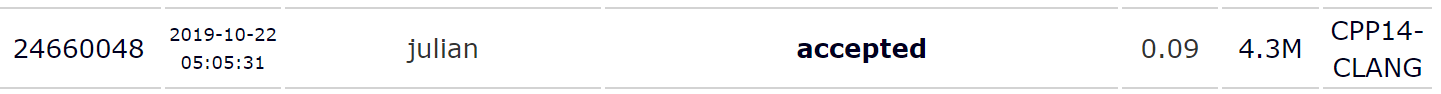
\includegraphics [width=\columnwidth]{bab5/img/hasil-uji-coba-kebenaran-situs-penilaian-spoj}
	\caption {Hasil Uji Coba Kebenaran Situs Penilaian Sphere Online Judge}
	\label {fig:hasil-uji-coba-kebenaran-situs-penilaian-spoj}
\end{figure}

\section{Uji Coba Kinerja Lokal}
Pada subbab ini akan ditampilkan hasil uji coba kinerja dari algoritma reduksi polygon untuk menyelesaikan permasalahan LL and ErBao. Pengujian dilakukan terhadap kelompok masukan yang telah dijelaskan pada subbab \ref{sec:skenario-uji-coba}. Detil masukan dapat dilihat pada Lampiran A. Langkah pengujian kinerja dilakukan dengan langkah sebagai berikut:
\begin{enumerate}
	\item Rekam waktu tepat sebelum komputasi penyelesaian masalah.
	\item Melakukan komputasi penyelesaian masalah untuk masukan kasus uji yang sama sebanyak 10 kali secara berturut-turut.
	\item Rekam waktu tepat setelah komputasi dengan mengurangi waktu selesai komputasi dengan waktu sebelum komputasi.
	\item Ulangi untuk semua kasus uji.
\end{enumerate}
\par Grafik \ref{fig:mean-running-time} menampilkan rata-rata kinerja masing-masing metode. Pada grafik tersebut dapat dilihat bahwa rata-rata \textit{running time} reduksi polygon dengan algoritma \textit{Melkman convex hull} berbanding lurus dengan banyaknya titik di dalam polygon tersebut.
\begin{figure}[!h]
	\Centering
	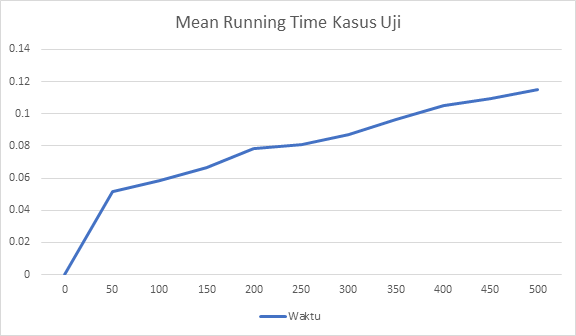
\includegraphics [width=\columnwidth]{bab5/img/mean-running-time}
	\caption {Grafik Mean Running Time Kasus Uji}
	\label {fig:mean-running-time}
\end{figure}

\section{Evaluasi Kebenaran Uji Coba Lokal}
Evaluasi dilakukan dengan memeriksa hasil keluaran program apakah sama dengan contoh keluaran pada Sphere Online Judge 5637 LL and ErBao. Tabel kebenaran dapat dilihat pada gambar \ref{tab:masukan-dan-keluaran-contoh-1}

\begin{table}[]
	\Centering
	\begin{tabular}{|l|c|}
	\hline
	\multicolumn{1}{|l|}{Data Masukan}  & Hasil Keluaran \\ \hline
	\begin{tabular}[l]{@{}l@{}}8 2\\ 0 0\\ 30 0\\ 30 20\\ 20 20\\ 20 10\\ 10 10\\ 10 20\\ 0 20\\ 5 15\\ 25 15\end{tabular} & Case \#1: 48.284          \\ \hline
	\end{tabular}
	\caption{Tabel Data Uji Coba Kebenaran Lokal dengan Sampel Data }
	\label{tab:masukan-dan-keluaran-contoh-1}
\end{table}

\par Gambar \ref{fig:kondisi-awal} menunjukan ilustrasi kondisi awal program sebelum iterasi dimulai.
\begin{figure}[!h]
	\Centering
	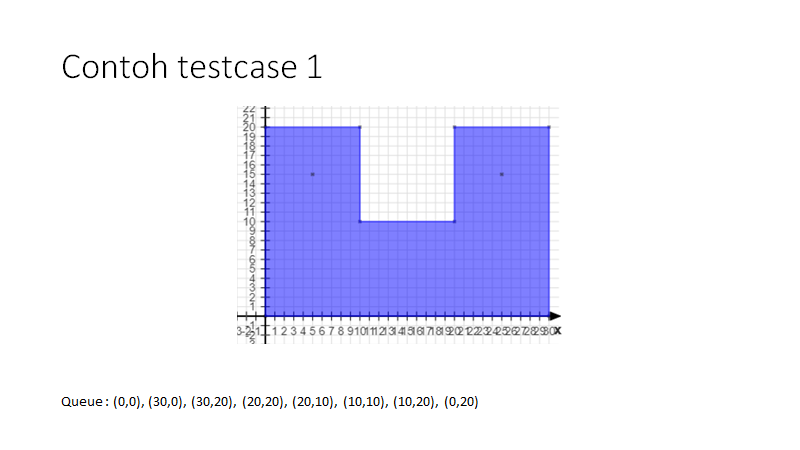
\includegraphics [width=\columnwidth]{bab5/img/kondisi-awal}
	\caption {Ilustrasi Kondisi Awal}
	\label {fig:kondisi-awal}
\end{figure}

\par Pada awal iterasi ke-1, memeriksa titik $(0,0)$. Titik tersebut akan dibuang karena titik tersebut merupakan titik luar dan orientasi terhadap titik sebelumnya dan sesudahnya membentuk \textit{convex}. Sebelum membuang titik tersebut, program membuat segitiga dengan titik sebelumnya, titik tersebut dan titik sesudahnya. Kemudian program mencari semua titik yang berada di dalam segitiga tersebut. Selanjutnya program mencari \textit{convex hull} dari semua titik yang didapatkan dan disisipkan ke queue polygon luar untuk menggantikan titik yang dibuang. Kondisi setelah iterasi ke-1 dapat dilihat pada gambar \ref{fig:iterasi-1}.
\begin{figure}[!h]
	\Centering
	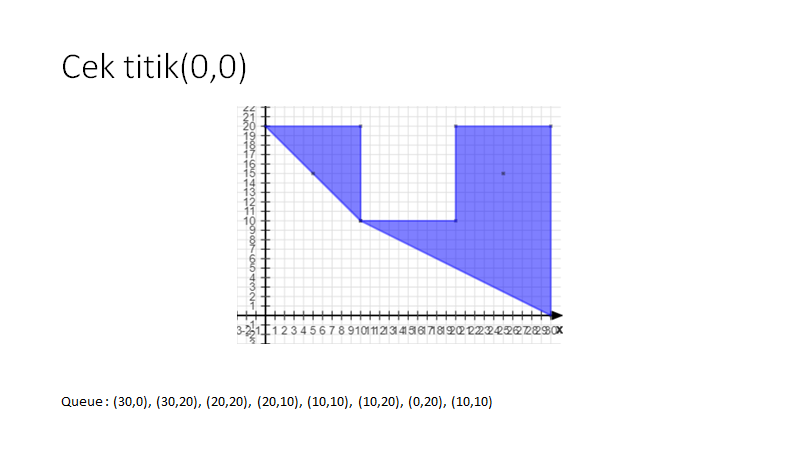
\includegraphics [width=\columnwidth]{bab5/img/iterasi-1}
	\caption {Ilustrasi Iterasi 1}
	\label {fig:iterasi-1}
\end{figure}

\par Pada awal iterasi ke-2, memeriksa titik $(30,0)$. Titik tersebut akan dibuang karena titik tersebut merupakan titik luar dan orientasi terhadap titik sebelumnya dan sesudahnya membentuk \textit{convex}. Sebelum membuang titik tersebut, program membuat segitiga dengan titik sebelumnya, titik tersebut dan titik sesudahnya. Kemudian program mencari semua titik yang berada di dalam segitiga tersebut. Selanjutnya program mencari \textit{convex hull} dari semua titik yang didapatkan dan disisipkan ke queue polygon luar untuk menggantikan titik yang dibuang. Kondisi setelah iterasi ke-2 dapat dilihat pada gambar \ref{fig:iterasi-2}.
\begin{figure}[!h]
	\Centering
	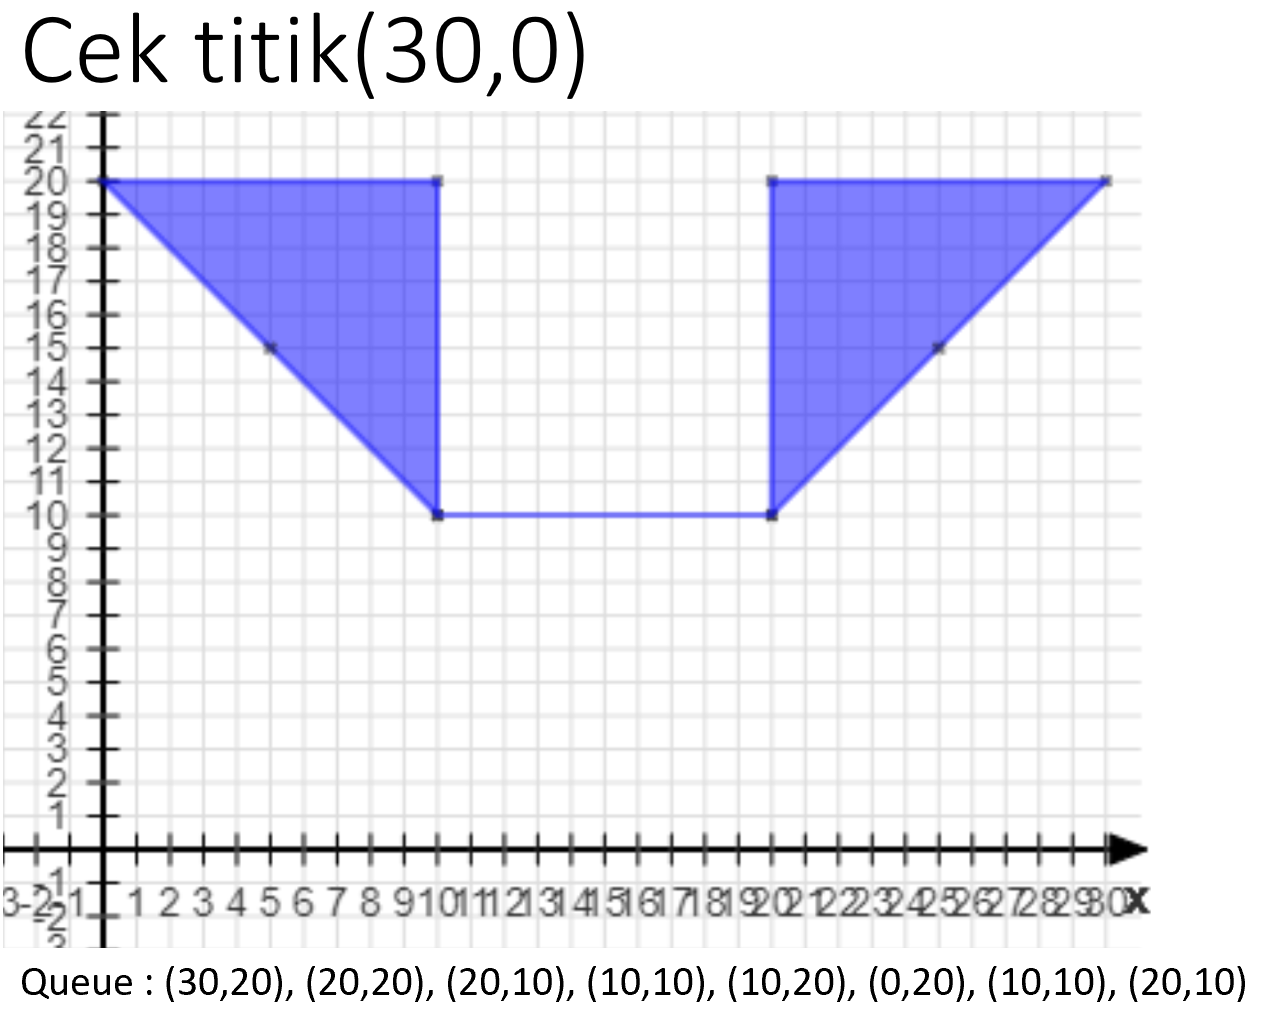
\includegraphics [width=\columnwidth]{bab5/img/iterasi-2}
	\caption {Ilustrasi Iterasi 2}
	\label {fig:iterasi-2}
\end{figure}

\par Pada awal iterasi ke-3, memeriksa titik $(30,20)$. Titik tersebut akan dibuang karena titik tersebut merupakan titik luar dan orientasi terhadap titik sebelumnya dan sesudahnya membentuk \textit{convex}. Sebelum membuang titik tersebut, program membuat segitiga dengan titik sebelumnya, titik tersebut dan titik sesudahnya. Kemudian program mencari semua titik yang berada di dalam segitiga tersebut. Selanjutnya program mencari \textit{convex hull} dari semua titik yang didapatkan dan disisipkan ke queue polygon luar untuk menggantikan titik yang dibuang. Kondisi setelah iterasi ke-3 dapat dilihat pada gambar \ref{fig:iterasi-3}.
\begin{figure}[!h]
	\Centering
	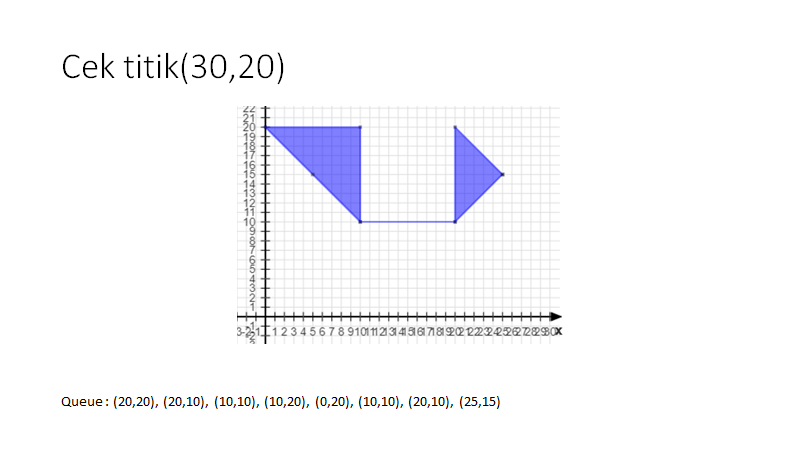
\includegraphics [width=\columnwidth]{bab5/img/iterasi-3}
	\caption {Ilustrasi Iterasi 3}
	\label {fig:iterasi-3}
\end{figure}

\par Pada awal iterasi ke-4, memeriksa titik $(20,20)$. Titik tersebut akan dibuang karena titik tersebut merupakan titik luar dan orientasi terhadap titik sebelumnya dan sesudahnya membentuk \textit{convex}. Sebelum membuang titik tersebut, program membuat segitiga dengan titik sebelumnya, titik tersebut dan titik sesudahnya. Kemudian program mencari semua titik yang berada di dalam segitiga tersebut. Selanjutnya program mencari \textit{convex hull} dari semua titik yang didapatkan dan disisipkan ke queue polygon luar untuk menggantikan titik yang dibuang. Kondisi setelah iterasi ke-4 dapat dilihat pada gambar \ref{fig:iterasi-4}.
\begin{figure}[!h]
	\Centering
	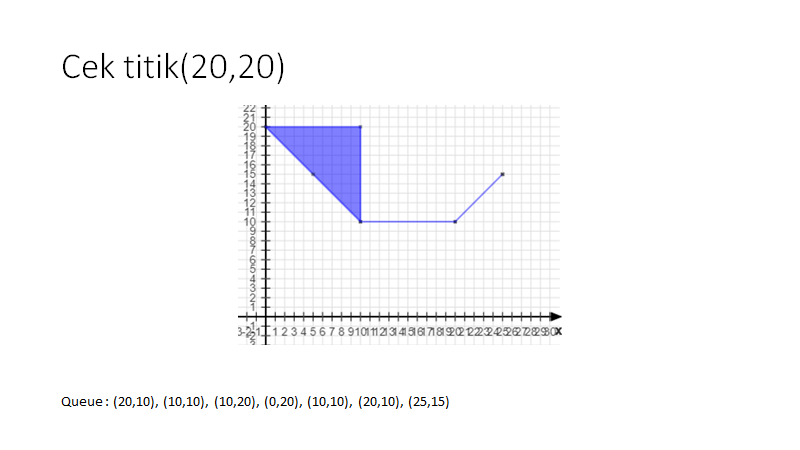
\includegraphics [width=\columnwidth]{bab5/img/iterasi-4}
	\caption {Ilustrasi Iterasi 4}
	\label {fig:iterasi-4}
\end{figure}

\par Pada awal iterasi ke-5, memeriksa titik $(20,10)$. Titik tersebut tidak akan dibuang karena titik tersebut merupakan titik luar tetapi orientasi terhadap titik sebelumnya dan sesudahnya membentuk \textit{concave}. Kondisi setelah iterasi ke-5 dapat dilihat pada gambar \ref{fig:iterasi-5}.
\begin{figure}[!h]
	\Centering
	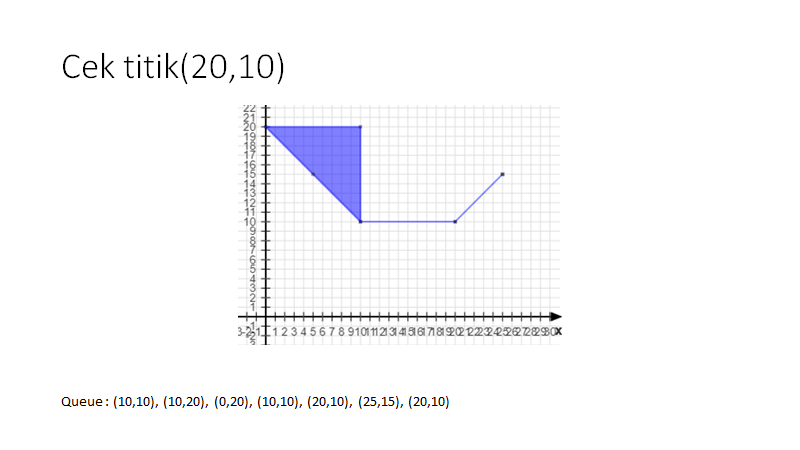
\includegraphics [width=\columnwidth]{bab5/img/iterasi-5}
	\caption {Ilustrasi Iterasi 5}
	\label {fig:iterasi-5}
\end{figure}

\par Pada awal iterasi ke-6, memeriksa titik $(10,10)$. Titik tersebut tidak akan dibuang karena titik tersebut merupakan titik luar tetapi orientasi terhadap titik sebelumnya dan sesudahnya membentuk \textit{concave}. Kondisi setelah iterasi ke-6 dapat dilihat pada gambar \ref{fig:iterasi-6}.
\begin{figure}[!h]
	\Centering
	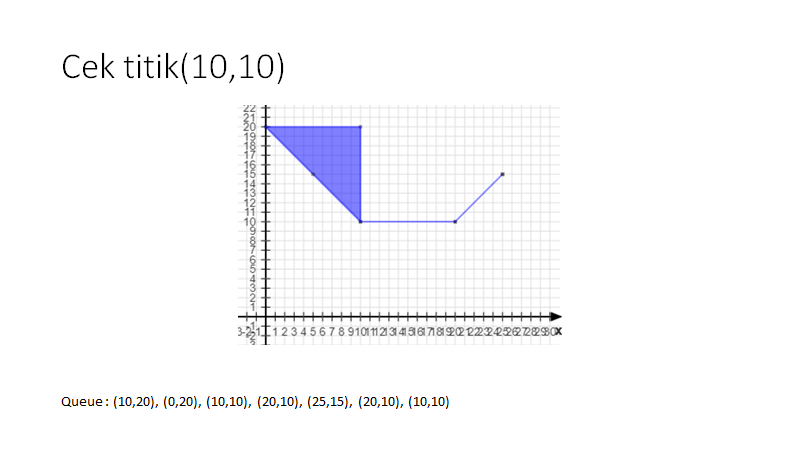
\includegraphics [width=\columnwidth]{bab5/img/iterasi-6}
	\caption {Ilustrasi Iterasi 6}
	\label {fig:iterasi-6}
\end{figure}

\par Pada awal iterasi ke-7, memeriksa titik $(10,20)$. Titik tersebut akan dibuang karena titik tersebut merupakan titik luar dan orientasi terhadap titik sebelumnya dan sesudahnya membentuk \textit{convex}. Sebelum membuang titik tersebut, program membuat segitiga dengan titik sebelumnya, titik tersebut dan titik sesudahnya. Kemudian program mencari semua titik yang berada di dalam segitiga tersebut. Selanjutnya program mencari \textit{convex hull} dari semua titik yang didapatkan dan disisipkan ke queue polygon luar untuk menggantikan titik yang dibuang. Kondisi setelah iterasi ke-7 dapat dilihat pada gambar \ref{fig:iterasi-7}.
\begin{figure}[!h]
	\Centering
	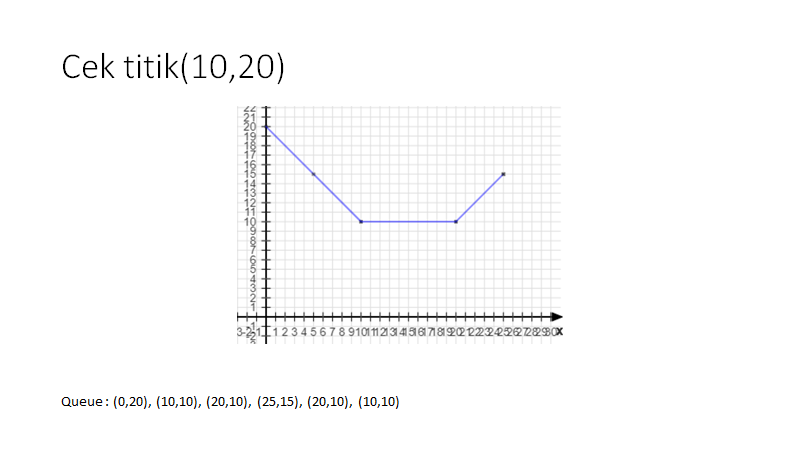
\includegraphics [width=\columnwidth]{bab5/img/iterasi-7}
	\caption {Ilustrasi Iterasi 7}
	\label {fig:iterasi-7}
\end{figure}

\par Pada awal iterasi ke-8, memeriksa titik $(0,20)$. Titik tersebut akan dibuang karena titik tersebut merupakan titik luar dan orientasi terhadap titik sebelumnya dan sesudahnya membentuk \textit{convex}. Sebelum membuang titik tersebut, program membuat segitiga dengan titik sebelumnya, titik tersebut dan titik sesudahnya. Kemudian program mencari semua titik yang berada di dalam segitiga tersebut. Selanjutnya program mencari \textit{convex hull} dari semua titik yang didapatkan dan disisipkan ke queue polygon luar untuk menggantikan titik yang dibuang. Kondisi setelah iterasi ke-8 dapat dilihat pada gambar \ref{fig:iterasi-8}.
\begin{figure}[!h]
	\Centering
	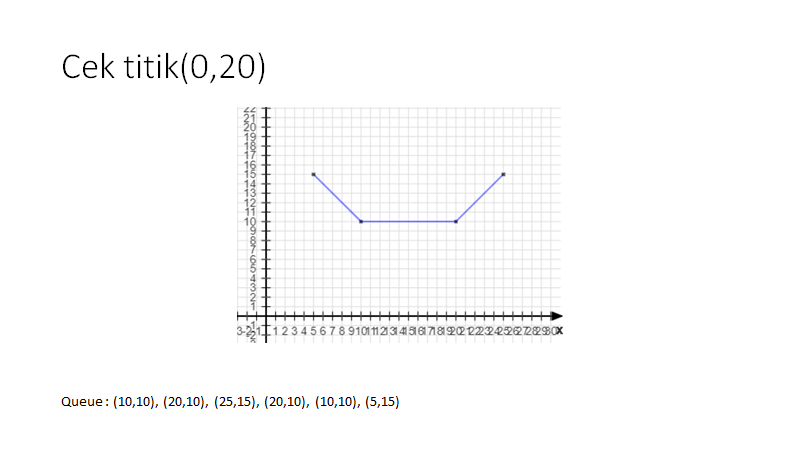
\includegraphics [width=\columnwidth]{bab5/img/iterasi-8}
	\caption {Ilustrasi Iterasi 8}
	\label {fig:iterasi-8}
\end{figure}

\section{Uji Coba Kinerja Luar}
Pada subbab ini akan ditampilkan hasil uji coba kinerja dari algoritma reduksi polygon. Pengujian dilakukan dengan cara mengirimkan kode program ke situs penilaian daring Sphere Online Judge. Detil mengenai hasil uji kinerja dapat dilihat pada Lampiran. Rata-rata hasil pengumpulan kode berkas dengan algoritma \textit{Melkman Convex Hull} adalah 0.08 detik dengan memori 4.6 MB. Hasil uji coba pada situs Sphere Online Judge dapat dilihat pada gambar \ref{fig:grafik-waktu-uji-coba-spoj} dan \ref{fig:grafik-memori-uji-coba-spoj}.
\begin{figure}[!h]
	\Centering
	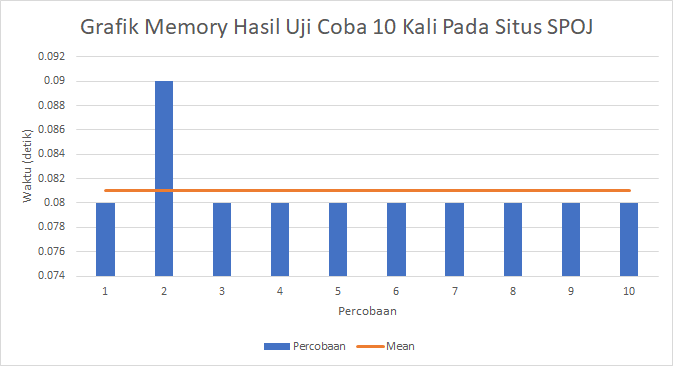
\includegraphics [width=\columnwidth]{bab5/img/grafik-waktu-uji-coba-spoj}
	\caption {Grafik Waktu Uji Coba 10 Kali pada Situs SPOJ}
	\label {fig:grafik-waktu-uji-coba-spoj}
\end{figure}
\begin{figure}[!h]
	\Centering
	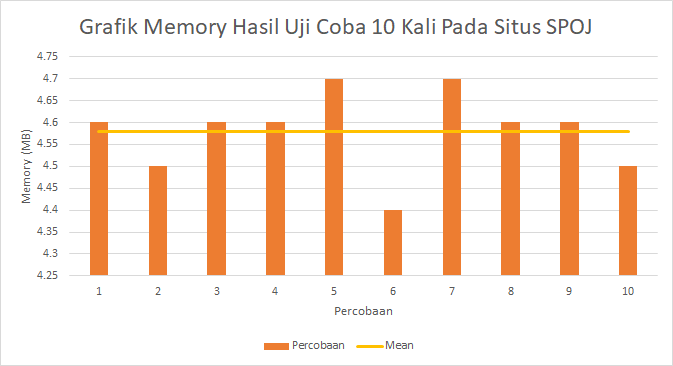
\includegraphics [width=\columnwidth]{bab5/img/grafik-memori-uji-coba-spoj}
	\caption {Grafik Memori Uji Coba 10 Kali pada Situs SPOJ}
	\label {fig:grafik-memori-uji-coba-spoj}
\end{figure}

 \cleardoublepage
		\chapter{KESIMPULAN}
Pada bab ini dijelaskan mengenai kesimpulan dari hasil uji coba yang telah dilakukan serta saran-saran tentang pengembangan yang dapat dilakukan terhadap Tugas Akhir ini di masa yang akan datang.
\section{ Kesimpulan}
Berdasarkan penjabaran di bab-bab sebelumnya, dapat disimpulkan beberapa poin terkait penyelesaian permasalahan LL and Erbao.
\begin{enumerate}
\item Permasalahan LL and ErBao dapat diselesaikan dengan melakukan reduksi polygon luar terhadap titik di dalamnya.
\item Permasalahan LL and Erbao dapat diselesaikan dengan batasan pada soal dapat diselesaikan dengan reduksi polygon dengan waktu minimum 0.08 detik, waktu maksimum 0.08 detik, dan memori minimum 4.4 MB, memori maksimum 4.7 MB.
\item Algoritma \textit{Melkman convex hull} terbukti efektif untuk melakukan reduksi polygon untuk mencari \textit{relative convex polygon}.
\end{enumerate}
\section{ Saran}
Pada Tugas Akhir kali ini tentunya terdapat kekurangan serta nilai-nilai yang dapat penulis ambil. Berikut adalah saran-saran yang dapat diambil melalui Tugas Akhir ini:
\begin{enumerate}
 \item Untuk kedepannya, algoritma pada Tugas Akhir ini dapat menjadi bahan riset untuk mencari optimasi lebih lanjut.
 \item Metode reduksi polygon dengan menggunakan algoritma \textit{Melkman convex hull} yang dimodifikasi dapat digunakan untuk mencari \textit{relative convex hull} dengan polygon yang membatasi segmen garis ataupun polygon sederhana.
\end{enumerate} \cleardoublepage
	
	\backmatter
	 	\printbibliography
		\chapter{LAMPIRAN A: DATA UJI}

\newcounter{tablepart}
\setcounter{tablepart}{1}
\setcounter{table}{0}
\renewcommand{\thetable}{A.\arabic{table}}

\begin{landscape}
	\begin{table}[]
		\begin{tabular}{|cccccc|}
		\hline
		\multicolumn{6} {|c|} {Data Masukan}\\ \hline
		-10000 -10000 & -9840 -10000 & -9680 -10000 & -9520 -10000 & -9360 -10000 & -9200 -10000\\
		-9040 -10000 & -8880 -10000 & -8720 -10000 & -8560 -10000 & -8400 -10000 & -8240 -10000\\
		-8080 -10000 & -7920 -10000 & -7760 -10000 & -7600 -10000 & -7440 -10000 & -7280 -10000\\
		-7120 -10000 & -6960 -10000 & -6800 -10000 & -6640 -10000 & -6480 -10000 & -6320 -10000\\
		-6160 -10000 & -6000 -10000 & -5840 -10000 & -5680 -10000 & -5520 -10000 & -5360 -10000\\
		-5200 -10000 & -5040 -10000 & -4880 -10000 & -4720 -10000 & -4560 -10000 & -4400 -10000\\
		-4240 -10000 & -4080 -10000 & -3920 -10000 & -3760 -10000 & -3600 -10000 & -3440 -10000\\
		-3280 -10000 & -3120 -10000 & -2960 -10000 & -2800 -10000 & -2640 -10000 & -2480 -10000\\
		-2320 -10000 & -2160 -10000 & -2000 -10000 & -1840 -10000 & -1680 -10000 & -1520 -10000\\
		-1360 -10000 & -1200 -10000 & -1040 -10000 & -880 -10000 & -720 -10000 & -560 -10000\\
		-400 -10000 & -240 -10000 & -80 -10000 & 80 -10000 & 240 -10000 & 400 -10000\\
		560 -10000 & 720 -10000 & 880 -10000 & 1040 -10000 & 1200 -10000 & 1360 -10000\\
		1520 -10000 & 1680 -10000 & 1840 -10000 & 2000 -10000 & 2160 -10000 & 2320 -10000\\
		2480 -10000 & 2640 -10000 & 2800 -10000 & 2960 -10000 & 3120 -10000 & 3280 -10000\\
		3440 -10000 & 3600 -10000 & 3760 -10000 & 3920 -10000 & 4080 -10000 & 4240 -10000\\
		4400 -10000 & 4560 -10000 & 4720 -10000 & 4880 -10000 & 5040 -10000 & 5200 -10000\\
		5360 -10000 & 5520 -10000 & 5680 -10000 & 5840 -10000 & 6000 -10000 & 6160 -10000\\
		6320 -10000 & 6480 -10000 & 6640 -10000 & 6800 -10000 & 6960 -10000 & 7120 -10000\\
		7280 -10000 & 7440 -10000 & 7600 -10000 & 7760 -10000 & 7920 -10000 & 8080 -10000\\
		8240 -10000 & 8400 -10000 & 8560 -10000 & 8720 -10000 & 8880 -10000 & 9040 -10000\\
		9200 -10000 & 9360 -10000 & 9520 -10000 & 9680 -10000 & 9840 -10000 & 10000 -10000\\
		10000 -9840 & 10000 -9680 & 10000 -9520 & 10000 -9360 & 10000 -9200 & 10000 -9040\\
		10000 -8880 & 10000 -8720 & 10000 -8560 & 10000 -8400 & 10000 -8240 & 10000 -8080\\
		10000 -7920 & 10000 -7760 & 10000 -7600 & 10000 -7440 & 10000 -7280 & 10000 -7120\\ \hline
        \end{tabular}
    \end{table}
\end{landscape}
\begin{landscape}
	\begin{table}[]
		\begin{tabular}{|cccccc|}
		\hline
		\multicolumn{6} {|c|} {Data Masukan}\\ \hline
		10000 -6960 & 10000 -6800 & 10000 -6640 & 10000 -6480 & 10000 -6320 & 10000 -6160\\
		10000 -6000 & 10000 -5840 & 10000 -5680 & 10000 -5520 & 10000 -5360 & 10000 -5200\\
		10000 -5040 & 10000 -4880 & 10000 -4720 & 10000 -4560 & 10000 -4400 & 10000 -4240\\
		10000 -4080 & 10000 -3920 & 10000 -3760 & 10000 -3600 & 10000 -3440 & 10000 -3280\\
		10000 -3120 & 10000 -2960 & 10000 -2800 & 10000 -2640 & 10000 -2480 & 10000 -2320\\
		10000 -2160 & 10000 -2000 & 10000 -1840 & 10000 -1680 & 10000 -1520 & 10000 -1360\\
		10000 -1200 & 10000 -1040 & 10000 -880 & 10000 -720 & 10000 -560 & 10000 -400\\
		10000 -240 & 10000 -80 & 10000 80 & 10000 240 & 10000 400 & 10000 560\\
		10000 720 & 10000 880 & 10000 1040 & 10000 1200 & 10000 1360 & 10000 1520\\
		10000 1680 & 10000 1840 & 10000 2000 & 10000 2160 & 10000 2320 & 10000 2480\\
		10000 2640 & 10000 2800 & 10000 2960 & 10000 3120 & 10000 3280 & 10000 3440\\
		10000 3600 & 10000 3760 & 10000 3920 & 10000 4080 & 10000 4240 & 10000 4400\\
		10000 4560 & 10000 4720 & 10000 4880 & 10000 5040 & 10000 5200 & 10000 5360\\
		10000 5520 & 10000 5680 & 10000 5840 & 10000 6000 & 10000 6160 & 10000 6320\\
		10000 6480 & 10000 6640 & 10000 6800 & 10000 6960 & 10000 7120 & 10000 7280\\
		10000 7440 & 10000 7600 & 10000 7760 & 10000 7920 & 10000 8080 & 10000 8240\\
		10000 8400 & 10000 8560 & 10000 8720 & 10000 8880 & 10000 9040 & 10000 9200\\
		10000 9360 & 10000 9520 & 10000 9680 & 10000 9840 & 10000 10000 & 9840 10000\\
		9680 10000 & 9520 10000 & 9360 10000 & 9200 10000 & 9040 10000 & 8880 10000\\
		8720 10000 & 8560 10000 & 8400 10000 & 8240 10000 & 8080 10000 & 7920 10000\\
		7760 10000 & 7600 10000 & 7440 10000 & 7280 10000 & 7120 10000 & 6960 10000\\
		6800 10000 & 6640 10000 & 6480 10000 & 6320 10000 & 6160 10000 & 6000 10000\\
		5840 10000 & 5680 10000 & 5520 10000 & 5360 10000 & 5200 10000 & 5040 10000\\
		4880 10000 & 4720 10000 & 4560 10000 & 4400 10000 & 4240 10000 & 4080 10000\\ \hline
        \end{tabular}
    \end{table}
\end{landscape}
\begin{landscape}
	\begin{table}[]
		\begin{tabular}{|cccccc|}
		\hline
		\multicolumn{6} {|c|} {Data Masukan}\\ \hline
		3920 10000 & 3760 10000 & 3600 10000 & 3440 10000 & 3280 10000 & 3120 10000\\
		2960 10000 & 2800 10000 & 2640 10000 & 2480 10000 & 2320 10000 & 2160 10000\\
		2000 10000 & 1840 10000 & 1680 10000 & 1520 10000 & 1360 10000 & 1200 10000\\
		1040 10000 & 880 10000 & 720 10000 & 560 10000 & 400 10000 & 240 10000\\
		80 10000 & -80 10000 & -240 10000 & -400 10000 & -560 10000 & -720 10000\\
		-880 10000 & -1040 10000 & -1200 10000 & -1360 10000 & -1520 10000 & -1680 10000\\
		-1840 10000 & -2000 10000 & -2160 10000 & -2320 10000 & -2480 10000 & -2640 10000\\
		-2800 10000 & -2960 10000 & -3120 10000 & -3280 10000 & -3440 10000 & -3600 10000\\
		-3760 10000 & -3920 10000 & -4080 10000 & -4240 10000 & -4400 10000 & -4560 10000\\
		-4720 10000 & -4880 10000 & -5040 10000 & -5200 10000 & -5360 10000 & -5520 10000\\
		-5680 10000 & -5840 10000 & -6000 10000 & -6160 10000 & -6320 10000 & -6480 10000\\
		-6640 10000 & -6800 10000 & -6960 10000 & -7120 10000 & -7280 10000 & -7440 10000\\
		-7600 10000 & -7760 10000 & -7920 10000 & -8080 10000 & -8240 10000 & -8400 10000\\
		-8560 10000 & -8720 10000 & -8880 10000 & -9040 10000 & -9200 10000 & -9360 10000\\
		-9520 10000 & -9680 10000 & -9840 10000 & -10000 10000 & -10000 9840 & -10000 9680\\
		-10000 9520 & -10000 9360 & -10000 9200 & -10000 9040 & -10000 8880 & -10000 8720\\
		-10000 8560 & -10000 8400 & -10000 8240 & -10000 8080 & -10000 7920 & -10000 7760\\
		-10000 7600 & -10000 7440 & -10000 7280 & -10000 7120 & -10000 6960 & -10000 6800\\
		-10000 6640 & -10000 6480 & -10000 6320 & -10000 6160 & -10000 6000 & -10000 5840\\
		-10000 5680 & -10000 5520 & -10000 5360 & -10000 5200 & -10000 5040 & -10000 4880\\
		-10000 4720 & -10000 4560 & -10000 4400 & -10000 4240 & -10000 4080 & -10000 3920\\
		-10000 3760 & -10000 3600 & -10000 3440 & -10000 3280 & -10000 3120 & -10000 2960\\
		-10000 2800 & -10000 2640 & -10000 2480 & -10000 2320 & -10000 2160 & -10000 2000\\
		-10000 1840 & -10000 1680 & -10000 1520 & -10000 1360 & -10000 1200 & -10000 1040\\ \hline
        \end{tabular}
    \end{table}
\end{landscape}
\begin{landscape}
	\begin{table}[]
		\begin{tabular}{|cccccc|}
		\hline
		\multicolumn{6} {|c|} {Data Masukan}\\ \hline
		-10000 880 & -10000 720 & -10000 560 & -10000 400 & -10000 240 & -10000 80\\
		-10000 -80 & -10000 -240 & -10000 -400 & -10000 -560 & -10000 -720 & -10000 -880\\
		-10000 -1040 & -10000 -1200 & -10000 -1360 & -10000 -1520 & -10000 -1680 & -10000 -1840\\
		-10000 -2000 & -10000 -2160 & -10000 -2320 & -10000 -2480 & -10000 -2640 & -10000 -2800\\
		-10000 -2960 & -10000 -3120 & -10000 -3280 & -10000 -3440 & -10000 -3600 & -10000 -3760\\
		-10000 -3920 & -10000 -4080 & -10000 -4240 & -10000 -4400 & -10000 -4560 & -10000 -4720\\
		-10000 -4880 & -10000 -5040 & -10000 -5200 & -10000 -5360 & -10000 -5520 & -10000 -5680\\
		-10000 -5840 & -10000 -6000 & -10000 -6160 & -10000 -6320 & -10000 -6480 & -10000 -6640\\
		-10000 -6800 & -10000 -6960 & -10000 -7120 & -10000 -7280 & -10000 -7440 & -10000 -7600\\
		-10000 -7760 & -10000 -7920 & -10000 -8080 & -10000 -8240 & -10000 -8400 & -10000 -8560\\
		-10000 -8720 & -10000 -8880 & -10000 -9040 & -10000 -9200 & -10000 -9360 & -10000 -9520\\
		-10000 -9680 & -10000 -9840 & -10000 -9840 & -10000 -9840 & -10000 -9840 & -10000 -9840\\ \hline
        \end{tabular}
    \end{table}
\end{landscape}

\begin{landscape}
	\begin{table}[]
		\begin{tabular}{|c|ccccc|c|}
		\hline
		No & \multicolumn{5} {c|} {Data Masukan} & Hasil Keluaran \\ \hline
		\multirow{10}{*}{1} & 7297 -5179 & -2569 -3179 & 4094 3274 & 719 -1563 & -6680 348 & \multirow{10}{*}{PASS} \\
				 & 8612 8164 & 4715 6559 & 7379 -4515 & -1673 -453 & 4384 1550 & 		 \\
				 & -9492 2456 & 8566 -7924 & -5067 8717 & -348 -6272 & -9614 7411 & 		 \\
				 & -7094 2912 & -1607 -8546 & -8967 3377 & 7968 -6804 & 4502 2445 & 		 \\
				 & -522 -5220 & -9762 -2864 & -9553 -7675 & -2831 9356 & -5142 -8928 & 		 \\
				 & 1322 -7910 & 3468 5862 & -3159 -7017 & -6292 2816 & -6690 9999 & 		 \\
				 & -4586 2554 & -8768 -5072 & 8616 1655 & 122 -6517 & -5057 366 & 		 \\
				 & 427 9209 & -1959 -8021 & -9683 2936 & -2060 1045 & -5261 -710 & 		 \\
				 & 1589 -3109 & -9898 8125 & -8467 -3993 & -6508 -803 & -9344 -8748 & 		 \\
				 & 848 -6711 & 2014 -7074 & -8930 -5099 & -2573 -7553 & -5884 2478 & 		 \\ \hline
        \multirow{20}{*}{2} & 1077 -4209 & 811 -5936 & -9315 -722 & 3288 -7436 & 2351 1858 & \multirow{20}{*}{PASS} \\
                & 4669 -4219 & -7102 -6866 & 443 -2655 & -7890 6739 & 2139 549 & 		 \\
                & -315 7509 & 6470 -3119 & 3990 -5881 & 4775 6120 & 4932 4153 & 		 \\
                & 8799 1869 & -7971 -8298 & -7431 -2162 & -697 2220 & -2369 9155 & 		 \\
                & -2883 -4402 & 6095 5840 & -2951 1527 & -1431 -9392 & -9263 -4014 & 		 \\
                & 9932 -5737 & -2457 -2634 & -1697 -2099 & -6979 469 & 2322 7104 & 		 \\
				 & 1693 -2996 & 3774 -4563 & -7785 189 & -1638 1867 & -8374 984 & 		 \\
				 & 827 4990 & -5251 -4969 & 2591 424 & -9503 -1857 & -4563 -6567 & 		 \\
				 & -8170 9456 & 2023 202 & -9101 -6438 & 8055 -6072 & -1446 -1076 & 		 \\
				 & -5018 -2154 & 4180 277 & 760 -1460 & -5826 -5307 & -6511 3749 & 		 \\
				 & 2911 -7372 & -457 -2377 & -4228 -1306 & 2046 -6622 & -4880 2668 & 		 \\
				 & 7905 8624 & 1560 -3250 & -1171 788 & 6027 5097 & 6690 -4013 & 		 \\
				 & 401 8884 & 4796 -9111 & -8909 1862 & -9652 -8018 & -6061 -7140 & 		 \\
				 & -3536 -9905 & 4246 -6408 & -8870 -9661 & -7387 6087 & -4016 -446 & 		 \\ \hline
		\end{tabular}
	\end{table}
\end {landscape}

\setcounter{tablepart}{1}
\setcounter{table}{0}
\renewcommand{\thetable}{A.\arabic{table}}
\begin{landscape}
	\begin{table}[]
		\begin{tabular}{|c|ccccc|c|}
		\hline
		No & \multicolumn{5} {c|} {Data Masukan} & Hasil Keluaran \\ \hline
				 & 7078 -2507 & -3894 510 & -6814 -833 & -433 1790 & -4181 -2535 & 		 \\
				 & -9517 -6848 & -8055 -336 & 8336 -170 & -6673 9657 & -6677 9221 & 		 \\
				 & -926 728 & 3780 -2491 & 9876 -2145 & -8026 7471 & -1095 6075 & 		 \\
				 & -8255 -9737 & -8773 -436 & 4348 -4649 & -6041 754 & -4925 -8434 & 		 \\
				 & -6326 -1839 & -5274 3881 & 9697 -8594 & -3225 1665 & -2355 9560 & 		 \\
				 & -1241 6405 & 806 9132 & 44 -1512 & 9233 -4679 & 1922 1663 & 		 \\ \hline
        \multirow{30}{*}{3} & 8761 -4183 & -3291 -6862 & 2098 3491 & -7363 -2537 & 5936 -9889 & \multirow{30}{*}{PASS} \\
                & 2045 -4180 & 5072 8708 & -153 1119 & 1925 7036 & 3217 2863 & 		 \\
                & -6398 -1990 & -1903 -3155 & -7243 6177 & -8770 -7995 & -5322 7841 & 		 \\
                & -2916 696 & -1599 -6654 & -6929 4331 & -800 -2393 & 5234 -9979 & 		 \\
                & -628 -8789 & 5451 -7693 & 4471 5455 & 3581 -1871 & -2558 5304 & 		 \\
                & 1598 4903 & 9716 -3150 & -7315 -3346 & 9805 -2696 & -8931 -5124 & 		 \\
                & -2602 -4231 & 7478 -8387 & 8605 -6284 & -1445 -6206 & 2464 7012 & 		 \\
                & 6830 -2630 & -9463 2242 & 6356 -3555 & 7386 -8249 & 9363 9807 & 		 \\
                & 6696 976 & 8612 -6592 & -404 -5369 & 3972 -9381 & -7305 8512 & 		 \\
                & -5268 -167 & -9113 -3551 & -4477 -2382 & -2217 -378 & -941 -3806 & 		 \\
                & -357 -3326 & 1880 -6625 & 8685 -1973 & -7519 -3665 & 1826 7089 & 		 \\
                & -8815 317 & 8609 -5267 & 293 1511 & -301 -4734 & 3677 -2437 & 		 \\
                & 9279 1758 & -3535 -8477 & -6225 -832 & -2835 382 & 5368 -3039 & 		 \\
                & -4774 1424 & -4104 -3317 & -5094 3519 & 257 2127 & 6299 5939 & 		 \\
                & -6794 -2216 & 8642 8839 & -4111 -9544 & -9169 4801 & -8878 7787 & 		 \\
                & 1890 -8680 & 8425 7739 & 8664 -2943 & -1735 -7201 & 2877 2120 & 		 \\
                & -2652 5900 & 5854 -7529 & 1025 2247 & 8797 -6179 & -8980 -394 & 		 \\
                & 1192 -5551 & 4351 -6430 & -5845 -6606 & 9510 -8169 & -5307 -9739 & 		 \\ \hline
		\end{tabular}
	\end{table}
\end {landscape}
\begin{landscape}
	\begin{table}[]
		\begin{tabular}{|c|ccccc|c|}
		\hline
		No & \multicolumn{5} {c|} {Data Masukan} & Hasil Keluaran \\ \hline
				 & -2098 -6423 & 1529 -2662 & 30 -6882 & -8762 2174 & -501 -3128 & 		 \\
				 & 7034 -8872 & 2440 2577 & -2751 5852 & -4997 6460 & -732 3620 & 		 \\
				 & 7767 4265 & 5297 7983 & 9957 -9000 & -1483 -216 & 4227 5747 & 		 \\
				 & -2735 108 & -9583 -858 & -1652 -3927 & 2247 -8401 & 7781 -4928 & 		 \\
				 & -2738 -3969 & -8693 -3753 & 8681 -2603 & 6641 -8823 & -3088 2002 & 		 \\
				 & 2107 27 & -7224 -8594 & -9569 4055 & 2127 -2718 & -5719 -5646 & 		 \\ 
				 & -4176 7828 & 379 2415 & 1986 1640 & -6303 -406 & -5747 7322 & 		 \\
				 & -8900 880 & -4022 7278 & -9798 6859 & -402 3972 & 6002 6053 & 		 \\
				 & -3992 -557 & -1303 -3766 & 2123 -2164 & 3160 2640 & -9627 -791 & 		 \\
				 & -9331 -4941 & -4423 -4799 & 7853 486 & -2199 -7720 & -3773 9450 & 		 \\
				 & -5451 -8543 & -4014 -5580 & -9754 -35 & 9358 -7106 & -254 2947 & 		 \\
				 & -9012 6712 & 6187 -5532 & 3256 -1255 & 5668 -9201 & 966 641 & 		 \\ \hline
				 & 2529 -5807 & -9526 -9908 & -6042 -4144 & 7994 7122 & -156 -9767 & 		 \\
				 & 52 -7491 & -3046 -1832 & -3902 2969 & -4144 -2977 & 9538 -542 & 		 \\
				 & 212 938 & -834 2748 & -1497 2754 & 5854 219 & 6228 7622 & 		 \\
				 & 9024 -5144 & -8706 -6363 & -6810 -3866 & 8325 -2414 & -3665 3346 & 		 \\
				 & 2240 5395 & -7893 -8310 & 5995 -5672 & 5259 -9587 & 4328 9909 & 		 \\
				 & -6411 -948 & -4386 -7736 & -2049 855 & 7111 9371 & -900 -6500 & 		 \\
				 & -7734 368 & -8109 -5553 & -156 -1640 & -4401 -4471 & -5813 -6682 & 		 \\
				 & -7426 725 & 2326 -2748 & 5491 1703 & -3816 -5595 & -8211 -2576 & 		 \\
				 & -2069 -6884 & 889 -7184 & -6667 2091 & -4258 6219 & 7110 -9315 & 		 \\
				 & -2064 608 & 2591 -4424 & -1242 -2346 & -7559 -2385 & -2445 -5257 & 		 \\
				 & -1915 628 & 6830 9538 & 9264 3637 & 7956 3259 & 1352 -7738 & 		 \\
				 & -2192 7302 & 6150 -7683 & -3013 7732 & -1149 1532 & 2079 -9412 & 		 \\ \hline
		\end{tabular}
	\end{table}
\end {landscape}
 \begin{landscape}
	\begin{table}[]
		\begin{tabular}{|c|ccccc|c|}
		\hline
		No & \multicolumn{5} {c|} {Data Masukan} & Hasil Keluaran \\ \hline
		\multirow{16}{*}{4} & -4078 -4147 & -738 -6964 & -243 -1353 & -6795 -1068 & 3843 7899 & \multirow{16}{*}{PASS} \\
				 & 2028 -2667 & -2272 6383 & 2524 -4662 & 2014 -5435 & -3447 722 & 		 \\
				 & 6900 -4261 & -2792 8004 & 2532 -8062 & 947 748 & -3049 -9138 & 		 \\
				 & 9382 -3485 & 7679 2457 & -7268 -6755 & 958 738 & -4466 -3547 & 		 \\
				 & 1518 4821 & -3104 -1690 & 5239 9458 & 810 3724 & 1829 5445 & 		 \\
				 & -553 4300 & -9892 -4034 & 1100 -6850 & -1876 -6980 & -8757 4851 & 		 \\
				 & -381 7275 & -8426 -541 & -2624 -4528 & -9833 1704 & -7793 8098 & 		 \\
				 & -898 -5301 & 4688 9948 & -52 -2853 & 2459 9488 & -1457 -5978 & 		 \\
				 & -8319 2430 & 6064 8866 & 3349 4965 & -1110 8522 & -3573 9753 & 		 \\
				 & -6179 5040 & 7264 9046 & 4354 -2927 & 3419 -3661 & -322 9092 & 		 \\
				 & 3666 1563 & -9604 7799 & 2767 -1127 & -779 -4260 & -4461 7154 & 		 \\
				 & 1940 8736 & -8868 7831 & 1146 2236 & -7516 -4999 & -9637 -2513 & 		 \\
				 & 9739 -9023 & -7215 -3988 & 8119 985 & -9038 5617 & -9896 -5845 & 		 \\
				 & -8774 -7591 & -5873 -555 & 2609 3729 & 242 -5323 & 423 -5649 & 		 \\
				 & -5207 4159 & 9570 -5951 & -5251 -4167 & 5404 -7707 & -5228 -635 & 		 \\
				 & 421 -7368 & 1971 1243 & 6513 -7472 & 110 1691 & -1938 -498 & 		 \\
				 & 576 960 & 3508 -5746 & -7920 2778 & -414 -7550 & -5088 5079 & 		 \\
				 & 1830 -4994 & 230 3232 & -2113 -1869 & 3182 -9205 & 8286 -9182 & 		 \\
				 & 2698 -2099 & -6447 -5943 & -7957 -8561 & 9347 -5052 & -7440 -1979 & 		 \\
				 & -8099 7887 & -7015 666 & 9491 -8244 & -4291 -8080 & -8006 -6864 & 		 \\
				 & -7644 2439 & -611 -3602 & 1550 8125 & 8468 5598 & -9612 1718 & 		 \\
				 & 745 -3108 & 142 -1287 & -7865 7247 & -2276 -4601 & -2864 1996 & 		 \\
				 & 2786 -9379 & -8919 3612 & 4334 -5408 & -1891 -6820 & 7358 -4512 & 		 \\
				 & 1153 1412 & 4229 -9008 & -3918 -1014 & -7380 -9155 & 2472 3048 & 		 \\ \hline
		\end{tabular}
	\end{table}
\end {landscape}
\begin{landscape}
	\begin{table}[]
		\begin{tabular}{|c|ccccc|c|}
		\hline
		No & \multicolumn{5} {c|} {Data Masukan} & Hasil Keluaran \\ \hline
        & 3640 2240 & 9702 -3108 & -4852 5398 & -3569 5197 & -8210 -1176 & 		 \\
        & -1 -5835 & -6034 -4369 & -2375 1501 & -605 1467 & 7037 6854 & 		 \\
        & -935 -9647 & -6501 2117 & -4503 3446 & -9136 1595 & -8536 2728 & 		 \\
        & -8285 -6471 & -2014 -2123 & -3652 -6137 & 3752 871 & 6288 -2644 & 		 \\ \hline
        & -9665 -7729 & 8968 -4248 & 9979 9443 & -1855 -4692 & -9248 -5969 & 		 \\
        & 4697 9838 & 2607 -3247 & -3976 -3800 & -6569 -8111 & -7601 -1705 & 		 \\
        & 79 7182 & -6933 10 & -5947 3869 & -131 -5824 & -7493 1613 & 		 \\
        & -227 4075 & 9264 1167 & -4397 -1032 & -964 -9865 & -5166 9969 & 		 \\
        & -7872 8957 & -7000 -5471 & 1725 -9465 & 5845 -3687 & -6619 9802 & 		 \\
        & -6889 2738 & -7537 -3795 & 5167 5269 & -9393 7121 & 4256 7320 & 		 \\
        & -1115 -9939 & -6703 9066 & -7852 -1505 & -1502 -8943 & -9899 643 & 		 \\
        & 4627 6385 & 1708 -7143 & 6694 -6961 & -9188 9750 & 2827 8151 & 		 \\
        & -2312 -8012 & -2378 6395 & -6470 -1561 & -3498 -8963 & 2583 -4103 & 		 \\
        & -6015 -8593 & 2579 -2674 & -9996 -8551 & 1136 -5785 & -7493 -4101 & 		 \\
        & -1652 -9874 & -7189 -1709 & 5165 -1936 & 887 -7295 & -5420 -9978 & 		 \\
        & -7006 -6998 & -5191 -5894 & 3956 -7911 & -7048 -3065 & 2024 -115 & 		 \\
        & -1655 4608 & -9044 9103 & 4718 371 & 1963 1569 & -9008 2447 & 		 \\
        & -2875 4192 & -6517 1059 & -1534 2626 & 2921 -6168 & 9798 -8481 & 		 \\
        & 3341 5827 & -2139 -806 & 9649 8741 & 311 2229 & -1229 -6414 & 		 \\
        & 6639 1418 & -7927 -9877 & 7240 957 & -737 -1593 & 5666 -5333 & 		 \\
        & 2298 7005 & -9045 -9946 & -3654 1992 & -9374 3362 & -919 -887 & 		 \\
        & -9416 -174 & -5297 -7823 & -1737 -1746 & 1862 -1831 & -472 -8424 & 		 \\
        & 4623 -9166 & 7345 -4321 & 3331 709 & -452 7109 & 5772 9490 & 		 \\
        & 2461 -8675 & 1013 -4134 & -4460 -7275 & -6626 2020 & -4049 444 & 		 \\ \hline
    \end{tabular}
\end{table}
\end {landscape}
\begin{landscape}
	\begin{table}[]
		\begin{tabular}{|c|ccccc|c|}
		\hline
		No & \multicolumn{5} {c|} {Data Masukan} & Hasil Keluaran \\ \hline
		\multirow{10}{*}{5} & 4579 -4104 & -2828 -4106 & -1964 1664 & 7919 -6141 & 2221 -6826 & \multirow{10}{*}{PASS} \\
				 & -6446 -8921 & -8553 -8336 & -3371 9748 & -804 7092 & 2001 -1653 & 		 \\
				 & 3871 -7782 & 9189 -4674 & 7851 -6065 & 9831 -1737 & 5539 -1982 & 		 \\
				 & 5526 9787 & 1878 360 & 1323 -2575 & -5266 -4092 & 946 1381 & 		 \\
				 & 8204 -8666 & 2809 -7027 & -8688 -2097 & -4761 -563 & -2339 -8609 & 		 \\
				 & -6643 -2182 & -1217 -8728 & -9053 -6341 & -31 -4189 & -8116 -9388 & 		 \\
				 & 4942 -7063 & 2524 -5661 & -9966 6103 & -3971 -6995 & 1083 -8423 & 		 \\
				 & -1045 -9512 & 9419 -2964 & -5946 146 & -9178 861 & 3243 -3466 & 		 \\
				 & -1297 -9041 & -2981 -6217 & 1330 -6425 & -7842 5879 & -9021 256 & 		 \\
				 & 9933 -2864 & 3753 -4193 & -1624 256 & 5171 -6324 & -9583 -2112 & 		 \\
                 & -267 -2980 & -7721 5856 & -2590 -9831 & 4997 -4018 & 2018 -3934 & 		 \\
				 & -1838 -7328 & 3956 8080 & -3352 -2370 & -8541 -6630 & -5056 -3778 & 		 \\
				 & 3435 -5672 & 4281 1774 & -6207 -5906 & -3131 -9575 & 7200 1979 & 		 \\
				 & -3528 8491 & -3152 -6280 & -263 -9331 & 6 726 & -8066 -6092 & 		 \\
				 & -7917 781 & -1191 -4766 & 3607 2132 & -2676 36 & -3401 242 & 		 \\
				 & -5756 7452 & -7601 375 & 33 9506 & 1896 -9980 & 7420 -4629 & 		 \\
				 & 9775 690 & 1254 -6868 & -4324 -2032 & -2038 411 & -6341 -625 & 		 \\
				 & -3041 7319 & -2904 9981 & 3162 -4153 & -644 7662 & 8095 869 & 		 \\
				 & 1223 -8226 & -645 -1443 & 510 5436 & 8052 2290 & -8584 -7582 & 		 \\
				 & -3232 8036 & 1842 544 & -6187 -3506 & -4195 -3996 & 7394 -9838 & 		 \\
				 & -6162 -5900 & 3324 -8647 & -4901 -1095 & -3046 9941 & -6326 -4349 & 		 \\
				 & -5177 905 & -9344 5802 & -6259 -5908 & -6367 1777 & 5174 6890 & 		 \\
				 & 2617 -2737 & -167 1355 & -6380 -2257 & -2610 -2186 & -4906 2905 & 		 \\
				 & -8473 -3334 & -9463 -2933 & -3907 -6843 & -1325 -6678 & 5990 -4810 & 		 \\ \hline
        \end{tabular}
    \end{table}
\end {landscape}
\begin{landscape}
	\begin{table}[]
		\begin{tabular}{|c|ccccc|c|}
		\hline
		No & \multicolumn{5} {c|} {Data Masukan} & Hasil Keluaran \\ \hline
        & -9943 5823 & -7411 -7687 & -8537 -9190 & -767 -9779 & 4191 3164 & 		 \\
        & -8081 5293 & 401 5653 & -8402 1575 & 1883 -4472 & -6629 -6737 & 		 \\
        & 4980 567 & -538 -2790 & 309 3645 & -3222 4034 & -2185 2423 & 		 \\
        & -5567 881 & -6973 -7834 & -7079 8028 & -3452 -5127 & -7807 -7411 & 		 \\
        & 97 -7898 & -9207 -9114 & -5686 -8966 & -119 9955 & -1104 -6894 & 		 \\
        & -3808 -4065 & -7397 3240 & -1343 9626 & 728 -9295 & -3894 -7784 & 		 \\ \hline
        & -5480 -9013 & 8005 1793 & -1304 546 & -930 -120 & -2628 -8657 & 		 \\
        & 826 -7034 & 867 1370 & -1968 7226 & 5758 4586 & -4332 -2646 & 		 \\
        & 9222 -2640 & -8451 -28 & -694 -2943 & 8865 -7136 & -1893 -9365 & 		 \\
        & 2747 -9175 & -7931 737 & -9482 -290 & 4256 6297 & -3699 7956 & 		 \\
        & 8776 7255 & 6890 -2369 & 5606 3175 & 206 -5745 & 6650 -8464 & 		 \\
        & 7068 9345 & -2798 4842 & 2478 7310 & -3972 -4280 & -922 -5113 & 		 \\
        & 2044 249 & -3989 -7613 & 1441 -715 & -8012 8791 & -6955 1232 & 		 \\
        & -353 -7704 & -7889 -1612 & -7035 2621 & -5799 -1426 & -7086 -4200 & 		 \\
        & -1531 -1335 & -6256 4807 & -7553 9401 & -5341 8438 & -5331 1048 & 		 \\
        & 5243 9671 & -2351 -7498 & -3386 9125 & -6065 4459 & 1153 1621 & 		 \\
        & -2450 3921 & 1277 9165 & -9665 -7409 & -3082 -3799 & -6815 -8902 & 		 \\
        & -1852 -2948 & -4921 -7976 & 1947 8645 & -7339 6021 & -8502 7363 & 		 \\
        & -8405 -39 & -8120 1417 & -6942 9257 & 1393 -7946 & -6790 5006 & 		 \\
        & -3766 -4578 & -1006 5763 & 1358 -2451 & 9819 8626 & -4542 -8724 & 		 \\
        & -469 943 & 9292 -6844 & -2836 8585 & 5700 -9596 & 9821 -4715 & 		 \\
        & -1145 9118 & -7880 -4171 & -3178 -8265 & -9324 -324 & -1419 -8482 & 		 \\
        & 8040 -8348 & 7062 4829 & -5427 -9011 & -8551 -4243 & -9011 2 & 		 \\
        & 7540 -9074 & -9991 4537 & 2191 -1417 & 1589 63 & -7661 -2965 & 		 \\ \hline
        \end{tabular}
    \end{table}
\end{landscape}
\begin{landscape}
	\begin{table}[]
		\begin{tabular}{|c|ccccc|c|}
		\hline
        No & \multicolumn{5} {c|} {Data Masukan} & Hasil Keluaran \\ \hline
        \multirow{24}{*}{6} & 9870 -3794 & 9428 1822 & -2140 -1491 & -8028 -5371 & -4788 1678 & \multirow{24}{*}{PASS} \\
                & 4637 -2157 & -6011 -242 & 2849 -5996 & -1555 -7593 & -9422 4054 & 		 \\
                & 571 -6649 & -448 -8425 & 4012 -3656 & -4251 2201 & 40 -9641 & 		 \\
                & 4926 -8855 & -9038 -9897 & -8168 -5026 & -8679 3295 & 6513 1863 & 		 \\
                & -4719 131 & -675 -57 & 2152 -6404 & -6197 1821 & -6030 7090 & 		 \\
                & 5411 2749 & -5013 -2827 & -6002 1167 & -1996 -586 & -4511 9294 & 		 \\
                & -7453 -3821 & 7828 6765 & -3165 6702 & -7989 5413 & -8081 3810 & 		 \\
                & 6276 -1400 & -4283 -4075 & -696 663 & 1691 -1263 & 126 -2473 & 		 \\
                & 2866 -3152 & -1747 -3811 & -6390 -1899 & -4488 -1199 & -6730 9827 & 		 \\
                & 2730 7763 & 4082 1832 & 8247 -3049 & 4049 4956 & -4768 9079 & 		 \\
                & -7685 -7864 & -5195 9640 & 919 3591 & 9794 -8084 & 6183 -2927 & 		 \\
                & -8987 -5878 & -3792 151 & -6310 3165 & -379 -2196 & 581 -6232 & 		 \\
                & 7355 -925 & -4856 -1295 & 6684 4192 & -143 -688 & 4804 -7961 & 		 \\
                & -1255 4797 & -3931 6841 & -1616 -7504 & -6833 1408 & 6454 -8785 & 		 \\
                & -1104 -6776 & -2621 -4479 & 88 113 & -2188 -4701 & -8576 6211 & 		 \\
                & -1953 -9893 & 5578 -2240 & 4675 -9486 & -3448 6689 & -5785 -4866 & 		 \\
                & 4610 7002 & -2526 -3012 & -9100 1982 & -6054 -7799 & -6409 -7702 & 		 \\
                & -790 -3865 & 1731 -1635 & -1340 -6846 & -6095 -8283 & -1792 -2952 & 		 \\
                & -8412 7041 & 171 8307 & -661 -6109 & -767 -4517 & -7649 8243 & 		 \\
                & 2468 7690 & 2292 -934 & -6622 -2623 & -5776 -7362 & -9221 -2535 & 		 \\
                & -3371 2125 & -507 2620 & -8189 -2538 & -2289 2132 & -4095 -7107 & 		 \\
                & -1562 5700 & -390 -7730 & 501 -1930 & -6651 -1584 & -4530 437 & 		 \\
                & -8628 1566 & 880 3933 & -8315 -3437 & -2847 1582 & 7618 451 & 		 \\
                & -2242 6217 & 4496 -4143 & 1939 -6091 & -9573 -1794 & 9741 -5983 & 		 \\ \hline
        \end{tabular}
    \end{table}
\end{landscape}
\begin{landscape}
	\begin{table}[]
		\begin{tabular}{|c|ccccc|c|}
		\hline
        No & \multicolumn{5} {c|} {Data Masukan} & Hasil Keluaran \\ \hline
        & -655 -6561 & 3567 -8626 & -8088 -5101 & 1536 -7218 & 99 -4141 & 		 \\
        & -8464 -2199 & -1102 -5140 & -3631 -7202 & -9000 3529 & -4537 -5775 & 		 \\
        & 2353 2547 & 7175 -7166 & -7279 8638 & -4550 -8388 & -4206 -5157 & 		 \\
        & -4924 -4881 & -9206 564 & 7395 -2975 & 1849 8952 & 7065 -6655 & 		 \\
        & 5388 -6316 & -146 5597 & -1156 8419 & -4561 -7564 & -6537 -9658 & 		 \\
        & 2011 9358 & 6629 -2921 & -1855 6442 & -2621 251 & -2334 -9833 & 		 \\
        & 3057 2645 & -8069 2663 & 2899 -6652 & -7542 3971 & -302 2244 & 		 \\
        & -2939 -8423 & 1095 9528 & -3953 1914 & -2415 -7510 & 2483 -2551 & 		 \\
        & 76 -9678 & -6298 -9971 & -7194 1525 & 434 7082 & -6616 7888 & 		 \\
        & 497 -8687 & 4287 -7626 & 5342 -4142 & -3916 6581 & -4437 827 & 		 \\
        & -7330 -1920 & -1683 1276 & -358 7368 & 4480 -9560 & -7111 -8883 & 		 \\
        & 8710 -8349 & 3453 1427 & -3823 -4041 & -4291 -9448 & -3839 -3221 & 		 \\
        & -2098 614 & -6477 686 & 1251 6884 & -9005 3128 & -8682 1393 & 		 \\
        & 9488 -5423 & -9565 -6444 & -4488 -7309 & 1233 -5875 & -3453 464 & 		 \\
        & 4990 -5103 & 1517 -4693 & -8782 723 & 2113 -4138 & -5680 -9082 & 		 \\
        & -198 -461 & -295 -2332 & -8340 -1543 & 7113 -1017 & 2463 2111 & 		 \\
        & 1184 -3681 & -4258 -495 & -5944 -7674 & -1552 -7481 & -7853 8591 & 		 \\
        & -5915 1335 & -8956 9918 & 2356 -2101 & 9843 8219 & 7393 -4881 & 		 \\ \hline
        & -5436 -9161 & -8216 -8836 & 3267 9971 & -2505 -6070 & 8129 -6827 & 		 \\
        & -3694 -8385 & 7881 -3616 & 9091 1828 & 2233 -6874 & 3286 -5420 & 		 \\
        & -2410 361 & 4501 -6098 & -2019 2020 & 2545 -5080 & 7134 -4786 & 		 \\
        & -321 2763 & -8251 -8930 & -5401 5787 & -6377 9227 & -1130 -4138 & 		 \\
        & 7016 -7595 & -6627 -1987 & 6817 -1176 & -9996 -9351 & 930 3967 & 		 \\
        & -4034 -454 & -2058 104 & -8588 -1287 & 9882 -6810 & -3046 8553 & 		 \\ \hline
    \end{tabular}
\end{table}
\end{landscape}
\begin{landscape}
	\begin{table}[]
		\begin{tabular}{|c|ccccc|c|}
		\hline
        No & \multicolumn{5} {c|} {Data Masukan} & Hasil Keluaran \\ \hline
        & -131 -6403 & 6037 3594 & 849 8396 & -4287 1049 & -8644 -3245 & 		 \\
        & -3649 -4748 & 8562 -9347 & 619 1136 & 5409 737 & -3880 6708 & 		 \\
        & 9515 -4924 & -6507 -6588 & 24 1722 & 9678 -8836 & -1620 -3592 & 		 \\
        & -8646 -9663 & -9095 -1340 & -6416 -3792 & 4687 5736 & 765 -1629 & 		 \\
        & -5769 2131 & -4842 -244 & -9816 -1258 & -7128 -3073 & -9038 -7372 & 		 \\
        & -4907 -9253 & 8185 6139 & -2558 -3459 & -3897 3147 & -9653 -8420 & 		 \\
        & -3647 2877 & -8805 -8456 & -3270 2247 & -9512 -664 & -4698 1244 & 		 \\
        & -5500 -2945 & 82 2708 & -3996 -1465 & -1486 -2806 & -1033 -6317 & 		 \\
        & 9149 -3382 & 1138 -2218 & -6412 8238 & -5971 -5587 & -4889 -6081 & 		 \\
        & -3436 -2044 & 4188 -4801 & -668 -2503 & -6104 -1551 & -1288 -6790 & 		 \\
        & 6720 -8304 & 4607 -5708 & 5108 1916 & -6607 -3283 & -3367 3455 & 		 \\
        & -4219 -9647 & 168 2603 & -8806 -1203 & -1178 2148 & -354 3162 & 		 \\
        & -5020 -8641 & -5807 2555 & -6809 -7096 & 3262 9704 & -2678 202 & 		 \\
        & -5997 5099 & -3357 -5366 & 3411 -375 & -7196 -1802 & -2681 -6298 & 		 \\
        & -3164 4669 & 1430 -60 & -4644 1022 & 1525 747 & -8267 -1659 & 		 \\
        & -2976 5741 & -9694 6099 & -4344 -8088 & 3884 5214 & 7889 -3506 & 		 \\
        & -3541 -6247 & -5163 -7291 & -8007 692 & 7882 2186 & -2197 -5625 & 		 \\
        & -2900 -2374 & -6597 -7860 & 372 -1134 & -1119 1163 & -3352 -9612 & 		 \\
        & -8917 -1318 & -2633 2989 & -2547 -3452 & -3899 -4236 & -1232 -1719 & 		 \\
        & 2756 -8682 & -2577 5894 & -8221 -4751 & 1673 2967 & -372 1756 & 		 \\
        & -3501 2746 & -2455 -7407 & -2939 -5900 & 7238 -4093 & 2208 90 & 		 \\
        & 2109 4915 & -2383 -5269 & -9012 868 & -3319 -39 & 2765 5352 & 		 \\
        & -3205 -4815 & -5185 -8956 & -4670 -8806 & 5353 -1036 & -1733 -2985 & 		 \\ \hline
    \end{tabular}
\end{table}
\end{landscape}
\begin{landscape}
	\begin{table}[]
		\begin{tabular}{|c|ccccc|c|}
		\hline
        No & \multicolumn{5} {c|} {Data Masukan} & Hasil Keluaran \\ \hline
		\multirow{10}{*}{7} & 617 -3791 & 723 6919 & 1787 -3944 & 1812 -2258 & 1831 5422 & \multirow{10}{*}{PASS} \\
				 & -9569 -9528 & 1952 7220 & -2748 2514 & 2220 -4289 & 1300 -574 & 		 \\
				 & -4833 2644 & -8292 -4209 & -5942 510 & -7160 -9545 & -9982 1371 & 		 \\
				 & 5608 -6582 & 6135 -4065 & 8428 -6172 & 1961 -4166 & -4598 7770 & 		 \\
				 & -3656 -2977 & -8817 -1642 & 1757 -514 & -9688 -3802 & 5272 4594 & 		 \\
				 & -6295 1204 & 425 5280 & 5803 -4018 & -5950 1436 & -4716 -4816 & 		 \\
				 & -3843 -880 & 8382 -5790 & -8598 -2534 & -176 -5989 & 3629 -4525 & 		 \\
				 & -2735 5383 & 6919 -362 & 8480 -4978 & 1872 -8224 & -2628 2262 & 		 \\
				 & 4591 -234 & -8695 -7392 & 6243 -538 & 244 1659 & -6783 7087 & 		 \\
				 & 854 3609 & 8324 4866 & -4137 -7590 & 6431 -6358 & 2645 5521 & 		 \\
				 & -7753 -9846 & 71 -8507 & -9777 5670 & -4741 7961 & -4445 2405 & 		 \\
				 & 103 -1944 & 2234 -2828 & 61 -2637 & 949 2735 & -8097 -9506 & 		 \\
				 & 1933 2268 & -8810 2167 & -7427 -9192 & 1086 5272 & -5732 8023 & 		 \\
				 & -4828 -5361 & -1908 7687 & 1203 -5476 & 8473 -1613 & -5367 9788 & 		 \\
				 & -5570 -9776 & 8434 9669 & 2240 2452 & -9425 2607 & -7062 -6815 & 		 \\
				 & -8555 -37 & -4049 -4052 & -9125 9650 & 6098 2459 & 3639 484 & 		 \\
				 & -57 -4438 & -1374 -1699 & -6791 3666 & 4603 -8363 & -5203 -311 & 		 \\
				 & -5645 5473 & -4281 171 & -6685 -844 & -436 -9061 & -3613 -3231 & 		 \\
				 & -5497 9447 & 3323 -320 & -1456 1256 & -9166 -2797 & 617 -6893 & 		 \\
				 & -1396 -5527 & 6636 6442 & -6664 -6973 & -928 -7470 & 9705 7030 & 		 \\
				 & 4308 -531 & -7650 -2129 & -3290 -577 & 6725 -4387 & 9444 9366 & 		 \\
				 & -2618 -2771 & -7531 -3771 & -5286 4592 & 2199 1015 & -9540 6626 & 		 \\
				 & -1013 421 & -5147 3468 & -2193 2239 & 4273 -6775 & -6609 -3503 & 		 \\
				 & -3036 -4666 & -5900 -6519 & -1580 9425 & -5243 -5995 & -5570 -1429 & 		 \\ \hline
        \end{tabular}
\end{table}
\end{landscape}
\begin{landscape}
	\begin{table}[]
		\begin{tabular}{|c|ccccc|c|}
		\hline
        No & \multicolumn{5} {c|} {Data Masukan} & Hasil Keluaran \\ \hline
        & 5263 -5847 & -3619 8190 & -7973 6024 & -7877 85 & 3084 -5022 & 		 \\
        & 2728 -698 & -1407 -1220 & 2280 -5867 & -4931 1457 & -656 -1579 & 		 \\
        & 3306 -8905 & -6604 -7310 & -7816 -7292 & -228 -6773 & 5580 -3983 & 		 \\
        & -2313 7363 & -4843 -8579 & 848 -1031 & 5668 -2604 & 4775 5815 & 		 \\
        & -651 -175 & -3688 1736 & 722 -5824 & -960 -5363 & 312 -7703 & 		 \\
        & -7198 -5037 & -2279 5165 & 8740 2269 & -5916 -7705 & -4513 1960 & 		 \\
        & -2271 -7426 & -2921 -8242 & -9055 -8549 & -9879 -8758 & -2987 2226 & 		 \\
        & 1218 -2594 & -7170 1930 & -1001 5554 & -6043 -6855 & -2925 -5348 & 		 \\
        & 812 -112 & 7371 -1849 & -3323 854 & -712 -2319 & -990 4314 & 		 \\
        & -5178 -1043 & -7410 -3132 & 3143 1331 & 6425 -5783 & -754 -9898 & 		 \\
        & -3017 -5365 & -7272 4753 & 109 -8170 & -4018 264 & -284 2766 & 		 \\
        & 9354 -7414 & -1406 -951 & -651 -8195 & -5256 -4672 & 2362 -427 & 		 \\
        & 9852 -9470 & -2795 -5627 & -2856 2634 & -1490 -9444 & -8155 -8911 & 		 \\
        & 9607 229 & 2099 5894 & -2864 -6279 & 1450 -3010 & -4606 7732 & 		 \\
        & -7753 -3802 & -2901 -4416 & -2337 3234 & 743 1465 & -9609 -9874 & 		 \\
        & 3537 -972 & -2986 -3126 & -4359 9016 & -7093 -3081 & -4234 -7986 & 		 \\
        & -564 -4100 & -3 -6878 & -5520 -3252 & -6702 -1089 & 6333 1802 & 		 \\ \hline
        & -4907 -9253 & 8185 6139 & -2558 -3459 & -3897 3147 & -9653 -8420 & 		 \\
        & -3647 2877 & -8805 -8456 & -3270 2247 & -9512 -664 & -4698 1244 & 		 \\
        & -5500 -2945 & 82 2708 & -3996 -1465 & -1486 -2806 & -1033 -6317 & 		 \\
        & 9149 -3382 & 1138 -2218 & -6412 8238 & -5971 -5587 & -4889 -6081 & 		 \\
        & -3436 -2044 & 4188 -4801 & -668 -2503 & -6104 -1551 & -1288 -6790 & 		 \\
        & 6720 -8304 & 4607 -5708 & 5108 1916 & -6607 -3283 & -3367 3455 & 		 \\ \hline
    \end{tabular}
\end{table}
\end{landscape}
\begin{landscape}
	\begin{table}[]
		\begin{tabular}{|c|ccccc|c|}
		\hline
        No & \multicolumn{5} {c|} {Data Masukan} & Hasil Keluaran \\ \hline
        & -3694 -8385 & 7881 -3616 & 9091 1828 & 2233 -6874 & 3286 -5420 & 		 \\
        & -2410 361 & 4501 -6098 & -2019 2020 & 2545 -5080 & 7134 -4786 & 		 \\
        & -321 2763 & -8251 -8930 & -5401 5787 & -6377 9227 & -1130 -4138 & 		 \\
        & 7016 -7595 & -6627 -1987 & 6817 -1176 & -9996 -9351 & 930 3967 & 		 \\
        & -4034 -454 & -2058 104 & -8588 -1287 & 9882 -6810 & -3046 8553 & 		 \\
        & -131 -6403 & 6037 3594 & 849 8396 & -4287 1049 & -8644 -3245 & 		 \\
        & -3649 -4748 & 8562 -9347 & 619 1136 & 5409 737 & -3880 6708 & 		 \\
        & 9515 -4924 & -6507 -6588 & 24 1722 & 9678 -8836 & -1620 -3592 & 		 \\
        & -8646 -9663 & -9095 -1340 & -6416 -3792 & 4687 5736 & 765 -1629 & 		 \\
        & -5769 2131 & -4842 -244 & -9816 -1258 & -7128 -3073 & -9038 -7372 & 		 \\
        & -4219 -9647 & 168 2603 & -8806 -1203 & -1178 2148 & -354 3162 & 		 \\
        & -5020 -8641 & -5807 2555 & -6809 -7096 & 3262 9704 & -2678 202 & 		 \\
        & -5997 5099 & -3357 -5366 & 3411 -375 & -7196 -1802 & -2681 -6298 & 		 \\
        & -3164 4669 & 1430 -60 & -4644 1022 & 1525 747 & -8267 -1659 & 		 \\
        & -2976 5741 & -9694 6099 & -4344 -8088 & 3884 5214 & 7889 -3506 & 		 \\
        & -3541 -6247 & -5163 -7291 & -8007 692 & 7882 2186 & -2197 -5625 & 		 \\
        & -2900 -2374 & -6597 -7860 & 372 -1134 & -1119 1163 & -3352 -9612 & 		 \\
        & -8917 -1318 & -2633 2989 & -2547 -3452 & -3899 -4236 & -1232 -1719 & 		 \\
        & 2756 -8682 & -2577 5894 & -8221 -4751 & 1673 2967 & -372 1756 & 		 \\
        & -3501 2746 & -2455 -7407 & -2939 -5900 & 7238 -4093 & 2208 90 & 		 \\
        & 2109 4915 & -2383 -5269 & -9012 868 & -3319 -39 & 2765 5352 & 		 \\
        & -3205 -4815 & -5185 -8956 & -4670 -8806 & 5353 -1036 & -1733 -2985 & 		 \\
        & -9569 -9528 & 1952 7220 & -2748 2514 & 2220 -4289 & 1300 -574 & 		 \\
        & -4833 2644 & -8292 -4209 & -5942 510 & -7160 -9545 & -9982 1371 & 		 \\ \hline
        \end{tabular}
    \end{table}
\end{landscape}
\begin{landscape}
	\begin{table}[]
		\begin{tabular}{|c|ccccc|c|}
		\hline
        No & \multicolumn{5} {c|} {Data Masukan} & Hasil Keluaran \\ \hline
        \multirow{20}{*}{8} & 617 -3791 & 723 6919 & 1787 -3944 & 1812 -2258 & 1831 5422 & \multirow{20}{*}{PASS} \\
                     & -5436 -9161 & -8216 -8836 & 3267 9971 & -2505 -6070 & 8129 -6827 & 		 \\
                     & 5608 -6582 & 6135 -4065 & 8428 -6172 & 1961 -4166 & -4598 7770 & 		 \\
                     & -3656 -2977 & -8817 -1642 & 1757 -514 & -9688 -3802 & 5272 4594 & 		 \\
                     & -6295 1204 & 425 5280 & 5803 -4018 & -5950 1436 & -4716 -4816 & 		 \\
                     & -3843 -880 & 8382 -5790 & -8598 -2534 & -176 -5989 & 3629 -4525 & 		 \\
                     & -2735 5383 & 6919 -362 & 8480 -4978 & 1872 -8224 & -2628 2262 & 		 \\
                     & 4591 -234 & -8695 -7392 & 6243 -538 & 244 1659 & -6783 7087 & 		 \\
                     & 854 3609 & 8324 4866 & -4137 -7590 & 6431 -6358 & 2645 5521 & 		 \\
                     & -7753 -9846 & 71 -8507 & -9777 5670 & -4741 7961 & -4445 2405 & 		 \\
                     & 103 -1944 & 2234 -2828 & 61 -2637 & 949 2735 & -8097 -9506 & 		 \\
                     & 1933 2268 & -8810 2167 & -7427 -9192 & 1086 5272 & -5732 8023 & 		 \\
                     & -4828 -5361 & -1908 7687 & 1203 -5476 & 8473 -1613 & -5367 9788 & 		 \\
                     & -5570 -9776 & 8434 9669 & 2240 2452 & -9425 2607 & -7062 -6815 & 		 \\
                     & -8555 -37 & -4049 -4052 & -9125 9650 & 6098 2459 & 3639 484 & 		 \\
                     & -57 -4438 & -1374 -1699 & -6791 3666 & 4603 -8363 & -5203 -311 & 		 \\
                     & -5645 5473 & -4281 171 & -6685 -844 & -436 -9061 & -3613 -3231 & 		 \\
                     & -5497 9447 & 3323 -320 & -1456 1256 & -9166 -2797 & 617 -6893 & 		 \\
                     & -1396 -5527 & 6636 6442 & -6664 -6973 & -928 -7470 & 9705 7030 & 		 \\
                     & 4308 -531 & -7650 -2129 & -3290 -577 & 6725 -4387 & 9444 9366 & 		 \\
                     & -2618 -2771 & -7531 -3771 & -5286 4592 & 2199 1015 & -9540 6626 & 		 \\
                     & -1013 421 & -5147 3468 & -2193 2239 & 4273 -6775 & -6609 -3503 & 		 \\
                     & -3036 -4666 & -5900 -6519 & -1580 9425 & -5243 -5995 & -5570 -1429 & 		 \\
                     & 5263 -5847 & -3619 8190 & -7973 6024 & -7877 85 & 3084 -5022 & 		 \\ \hline            
        \end{tabular}
    \end{table}
\end{landscape}
\begin{landscape}
	\begin{table}[]
		\begin{tabular}{|c|ccccc|c|}
		\hline
        No & \multicolumn{5} {c|} {Data Masukan} & Hasil Keluaran \\ \hline
        & 2728 -698 & -1407 -1220 & 2280 -5867 & -4931 1457 & -656 -1579 & 		 \\
        & 3306 -8905 & -6604 -7310 & -7816 -7292 & -228 -6773 & 5580 -3983 & 		 \\
        & -2313 7363 & -4843 -8579 & 848 -1031 & 5668 -2604 & 4775 5815 & 		 \\
        & -651 -175 & -3688 1736 & 722 -5824 & -960 -5363 & 312 -7703 & 		 \\
        & -7198 -5037 & -2279 5165 & 8740 2269 & -5916 -7705 & -4513 1960 & 		 \\
        & -2271 -7426 & -2921 -8242 & -9055 -8549 & -9879 -8758 & -2987 2226 & 		 \\
        & 1218 -2594 & -7170 1930 & -1001 5554 & -6043 -6855 & -2925 -5348 & 		 \\
        & 812 -112 & 7371 -1849 & -3323 854 & -712 -2319 & -990 4314 & 		 \\
        & -5178 -1043 & -7410 -3132 & 3143 1331 & 6425 -5783 & -754 -9898 & 		 \\
        & -3017 -5365 & -7272 4753 & 109 -8170 & -4018 264 & -284 2766 & 		 \\
        & 9354 -7414 & -1406 -951 & -651 -8195 & -5256 -4672 & 2362 -427 & 		 \\
        & 9852 -9470 & -2795 -5627 & -2856 2634 & -1490 -9444 & -8155 -8911 & 		 \\
        & 9607 229 & 2099 5894 & -2864 -6279 & 1450 -3010 & -4606 7732 & 		 \\
        & -7753 -3802 & -2901 -4416 & -2337 3234 & 743 1465 & -9609 -9874 & 		 \\
        & 3537 -972 & -2986 -3126 & -4359 9016 & -7093 -3081 & -4234 -7986 & 		 \\
        & -564 -4100 & -3 -6878 & -5520 -3252 & -6702 -1089 & 6333 1802 & 		 \\
        & -1058 2173 & -3068 1612 & 2562 5059 & 5707 -6113 & 9899 1190 & 		 \\
        & 2154 -3731 & 2181 -302 & 1820 6203 & -8394 -3956 & -1939 -5450 & 		 \\
        & -412 -9579 & 5112 -7826 & -617 2000 & 9077 -446 & 1091 1960 & 		 \\
        & 6222 -6881 & -3194 -4307 & -6316 -1211 & -5454 5630 & -369 -8919 & 		 \\
        & 869 8459 & 3100 -3615 & -6848 -9862 & 339 -8934 & -1547 6506 & 		 \\
        & 5317 1965 & -2622 -4171 & -6000 2067 & 1373 -4164 & 907 8917 & 		 \\
        & 3120 2175 & -3739 -3574 & -7256 5515 & 783 9755 & 4584 -3818 & 		 \\
        & -7212 -2647 & -5950 5871 & 2962 883 & -2135 4242 & -7676 -6288 & 		 \\ \hline
        \end{tabular}
    \end{table}
\end{landscape}
\begin{landscape}
	\begin{table}[]
		\begin{tabular}{|c|ccccc|c|}
		\hline
        No & \multicolumn{5} {c|} {Data Masukan} & Hasil Keluaran \\ \hline
        & 8641 -8968 & -7012 610 & -9672 3194 & -6788 2961 & -1319 5323 & 		 \\
        & -2181 -8951 & -5922 -8566 & -6422 -7569 & -1018 1213 & -3427 -4618 & 		 \\ \hline
        & -5392 -9309 & 8330 536 & 604 -605 & 3153 7981 & -1114 -4996 & 		 \\
        & -980 3030 & -5105 -1368 & 148 3664 & 5941 -5566 & -9096 4573 & 		 \\
        & -1274 3362 & -2548 -4934 & -3343 -250 & 3459 -3025 & -3840 -207 & 		 \\
        & 3845 1933 & 4196 -5830 & -8554 -8137 & -9776 -7845 & 8673 -3465 & 		 \\
        & 5256 -9678 & -7376 5630 & 8027 -5527 & -7430 7045 & 2445 -3603 & 		 \\
        & -2368 2514 & -1318 -4634 & -6887 -2650 & -9032 -2105 & -5171 2218 & 		 \\
        & -9540 -5821 & -3937 -5200 & 257 -2495 & -561 541 & -3099 -7723 & 		 \\
        & 5822 -1792 & 5012 -9849 & -4494 6886 & -3385 -9868 & -7908 -2385 & 		 \\
        & 560 -8514 & -6759 2019 & -5166 1277 & 4695 6658 & 2091 -8233 & 		 \\
        & -9768 3771 & -3073 4818 & -2212 -9474 & -4563 7013 & 377 2355 & 		 \\
        & -1854 341 & 1805 -9653 & -2734 -7873 & 1592 -2346 & 1506 1392 & 		 \\
        & 4805 -2792 & 1289 253 & -7063 -8329 & -7690 273 & 1964 -4202 & 		 \\
        & 1111 -1440 & 3277 1672 & 401 2470 & -415 -6148 & -2605 4715 & 		 \\
        & -7234 -1313 & -6064 -347 & -9350 6755 & -5557 -7005 & 2476 8857 & 		 \\
        & -1235 -7707 & 219 -4826 & -2754 7891 & -4874 -8811 & 401 5319 & 		 \\
        & 7041 -5972 & -3744 -5430 & -5391 -3976 & 9882 4456 & -8391 -5099 & 		 \\
        & 5401 4507 & 2152 -3479 & -4358 75 & -4663 4910 & 2277 -325 & 		 \\
        & -3212 9781 & -9674 7902 & 199 -989 & 8822 -3001 & -5814 2055 & 		 \\
        & -1911 -2359 & -5602 -1881 & -9233 -963 & 8079 7000 & -8702 -3649 & 		 \\
        & -5332 -3153 & -6266 -2307 & 2811 -9860 & 2626 -5805 & 7365 -2955 & 		 \\
        & 1514 -1807 & -8103 9777 & -1119 7071 & -8272 -1801 & -3045 -5182 & 		 \\
        & -1233 -8651 & 1287 -7745 & 9162 -9772 & -6037 8608 & 1806 -6868 & 		 \\ \hline
        \end{tabular}
    \end{table}
\end{landscape}
\begin{landscape}
	\begin{table}[]
		\begin{tabular}{|c|ccccc|c|}
		\hline
        No & \multicolumn{5} {c|} {Data Masukan} & Hasil Keluaran \\ \hline
        & 274 -2476 & -5312 8245 & 9989 7452 & -2240 -7810 & 7350 -543 & 		 \\
        & -5580 -927 & -8254 -2485 & 3908 -8969 & -7016 -3086 & -5856 -3033 & 		 \\
        & -4108 5997 & -983 -9948 & -4398 5200 & 3278 26 & -9825 -964 & 		 \\
        & 2645 -1444 & -3407 -4402 & 9949 5164 & -4932 -101 & 5986 919 & 		 \\
        & -9733 -2272 & -8992 -3879 & -6891 -1517 & -9574 -5907 & -3583 -1666 & 		 \\
        & -8098 -2306 & -6806 -7412 & 1058 -1856 & -9198 772 & -654 -6370 & 		 \\
        & 2578 9016 & 6190 1939 & 9736 -8011 & -8917 124 & -4046 261 & 		 \\
        & -6492 1871 & 8760 -4267 & -4945 8069 & -8184 -7889 & 5030 -420 & 		 \\
        & -8410 492 & 113 -2493 & -3035 8524 & -7486 -497 & 6351 -8474 & 		 \\
        & -7682 6379 & -5109 -3652 & -3233 311 & 6110 3604 & 6614 9328 & 		 \\
        & 1874 -8829 & 9556 -1044 & -1161 -4310 & -8694 -7059 & -3672 -5946 & 		 \\
        & -4434 -4594 & -3858 -6429 & 706 9983 & 1388 -2096 & -3023 -1929 & 		 \\
        & -6895 2106 & -4967 -2712 & 4145 1778 & -7025 9071 & 9051 -6097 & 		 \\
        & -9824 3725 & -6334 -1797 & -2380 3387 & -8257 -4697 & -4841 -3719 & 		 \\
        & -520 -925 & -6916 6151 & -893 1548 & -6503 -2088 & 8422 -3292 & 		 \\
        & 5079 -2141 & -2847 7113 & 7150 125 & -4849 -2081 & -3382 -1852 & 		 \\
        & -1177 7376 & 7765 -9284 & -7287 -6731 & -2832 -2496 & -4360 4372 & 		 \\
        & 8835 7313 & 3588 -2356 & 8438 -1838 & -8022 -3346 & -3811 -6696 & 		 \\
        & -6660 -1680 & -9350 1242 & -4026 -5060 & -8256 -7662 & -8439 2029 & 		 \\
        & -9002 8607 & -149 3998 & -9508 -5851 & -4590 -8775 & 9168 3716 & 		 \\
        & -2677 -4585 & -2032 -8291 & -4656 -7895 & -9851 8918 & -9587 -621 & 		 \\
        & -6697 -2620 & -8039 6297 & 9031 -9339 & -3255 538 & -8517 -6641 & 		 \\
		\multirow{2}{*}{9} & -1401 -3788 & -7982 -7985 & 5713 6371 & -1116 854 & -4317 1933 & \multirow{2}{*}{PASS} \\
		& -7957 8773 & 6459 8806 & -8210 -9695 & 123 7089 & 2529 6033 & 		 \\ \hline
        \end{tabular}
    \end{table}
\end{landscape}
\begin{landscape}
	\begin{table}[]
		\begin{tabular}{|c|ccccc|c|}
		\hline
        No & \multicolumn{5} {c|} {Data Masukan} & Hasil Keluaran \\ \hline
        & -3912 -2738 & -8416 1979 & -4981 2660 & 3689 -3324 & -689 3195 & 		 \\
        & -239 9536 & 17 2280 & -1056 3304 & -2944 -5845 & 3569 8813 & 		 \\
        & -5849 -932 & 1340 -9780 & -8992 -7293 & -7080 1090 & -290 -8185 & 		 \\
        & -8445 -5406 & -3627 -6551 & -2628 4166 & -4135 -1264 & -3597 1282 & 		 \\
        & 1921 4137 & 4003 9663 & -3377 425 & 3964 2182 & 7538 5364 & 		 \\
        & -2523 -3238 & -1815 -5439 & -2494 -4148 & -7539 -7365 & -8781 -598 & 		 \\
        & 1258 -7411 & 9884 -7081 & 9965 -8519 & -7732 -2431 & -4030 6026 & 		 \\
        & 1816 9422 & -3458 -5048 & -4888 -3912 & -4229 2384 & -9995 411 & 		 \\
        & 7553 5223 & 3664 4108 & -3924 1382 & -857 7021 & -5397 -4550 & 		 \\
        & -2876 7614 & 3592 -8176 & 1622 -7275 & -1690 -7671 & -5388 -8429 & 		 \\
        & -9616 -171 & 8799 302 & -2289 -2785 & 9223 -1070 & -4772 711 & 		 \\
        & -1104 -7123 & 152 -6963 & 2551 -2871 & -9033 -9709 & -1839 2485 & 		 \\
        & -2813 6374 & -7533 -9176 & -9344 -7788 & 2488 -696 & -1173 -4671 & 		 \\
        & 1373 -3419 & -9654 6366 & -465 -2230 & 3167 7034 & -6134 -3435 & 		 \\
        & -2116 2706 & 1946 6344 & 2652 8176 & 421 -9638 & -3344 -5967 & 		 \\
        & -5750 -7120 & -5765 -3770 & -3990 7920 & -2952 128 & -4022 -6348 & 		 \\
        & -9565 -1818 & -785 -8738 & -6089 -630 & -3246 4780 & -9550 -8356 & 		 \\
        & -8200 -4373 & -8256 1052 & -5161 -2255 & 2809 -4395 & -8449 -7867 & 		 \\
        & 8227 9031 & -6822 -2687 & 8509 3141 & -3791 -1187 & -8580 -7135 & 		 \\
        & -8333 1410 & -6442 357 & -1037 838 & -2977 -9277 & -3503 -8 & 		 \\
        & 306 -8881 & 9946 -3461 & -2829 1483 & 1041 1423 & 947 5892 & 		 \\
        & -5618 -6507 & -3052 -6308 & 6792 -4300 & -8497 -3641 & -1552 -2793 & 		 \\
        & 5842 763 & -5857 -5444 & 4588 -2016 & 1137 487 & -4788 -7408 & 		 \\
        & 881 8411 & 2217 -1637 & -618 -6485 & -355 -4887 & 4559 -1939 & 		 \\ \hline
        \end{tabular}
    \end{table}
\end{landscape}
\begin{landscape}
	\begin{table}[]
		\begin{tabular}{|c|ccccc|c|}
		\hline
        No & \multicolumn{5} {c|} {Data Masukan} & Hasil Keluaran \\ \hline
        & -4939 -3097 & -1253 -2415 & 911 -9894 & 1947 -9103 & 8986 -328 & 		 \\
        & -7730 -472 & 4737 -7690 & -398 6312 & -5813 8964 & -4048 -9754 & 		 \\
        & -5340 8057 & -198 -2022 & -7302 -6424 & 886 9029 & -4701 573 & 		 \\
        & 2713 -3183 & -9818 -2364 & -3059 -9729 & 1624 7880 & -1186 -4067 & 		 \\
        & -2843 764 & 2451 -5707 & -2352 5213 & -747 3470 & -3777 2327 & 		 \\
        & -2216 111 & -6095 -3355 & -9064 1277 & -1294 8096 & -7838 -6192 & 		 \\
        & -5679 175 & 6135 5956 & 77 -8379 & -1811 3978 & -5351 -5235 & 		 \\
        & -9128 2945 & -7975 9087 & -7610 -22 & -6292 -843 & -9616 -4234 & 		 \\
        & -8403 -65 & -2063 -603 & -3399 -7362 & -3665 -4468 & -5771 -6681 & 		 \\
        & 608 -7627 & 3083 5448 & 6002 -1619 & -5517 -6479 & -4125 6616 & 		 \\
        & -1030 499 & -9554 1478 & 31 -2011 & -4814 -5621 & -1769 -9721 & 		 \\
        & -1939 -7957 & -2818 -9048 & -2589 147 & -1242 6763 & 296 2609 & 		 \\
        & 1997 -985 & 5020 -9732 & -5221 9902 & 6801 -2827 & -2592 -1935 & 		 \\
        & -1388 -111 & -6845 -3199 & -660 -1516 & -5347 -4646 & 861 3553 & 		 \\
        & -2179 -3302 & 6193 -3151 & -1415 -4328 & 8599 962 & 7038 -6572 & 		 \\
        & -6805 1778 & -4829 -3287 & -584 -5940 & 7722 -9271 & -6435 -9950 & 		 \\
        & 8829 -7189 & 875 -707 & -6340 -8162 & -9032 -1679 & -1894 -7038 & 		 \\
        & 1903 1813 & 2501 -5319 & -6298 -6159 & 2919 1688 & -876 8696 & 		 \\
        & -5079 -5440 & -6814 -3048 & -7747 -5388 & -3551 -1425 & -1891 -5660 & 		 \\
        & -2595 -3392 & -9776 -9080 & -399 3047 & 9293 -2539 & -710 4457 & 		 \\ \hline
        & -2484 2866 & 1090 -6060 & -2881 1786 & -6899 -9539 & -8260 -3407 & 		 \\
        & 4082 -2682 & -304 5985 & -1057 -1765 & -2719 -6897 & -4846 3129 & 		 \\ \hline
        \end{tabular}
    \end{table}
\end{landscape}
\begin{landscape}
	\begin{table}[]
		\begin{tabular}{|c|ccccc|c|}
		\hline
        No & \multicolumn{5} {c|} {Data Masukan} & Hasil Keluaran \\ \hline
        & -5348 -9457 & -7892 2674 & 5175 1586 & 1577 2031 & 2410 -3165 & 		 \\
        & -5501 -5555 & 1910 -6354 & -1560 -1734 & 2416 2975 & -8712 -5435 & 		 \\
        & 7096 6363 & -9597 8997 & -4667 4713 & -2861 -969 & -7580 -8395 & 		 \\
        & 776 1104 & -3358 -2730 & -4473 -9293 & -408 -4915 & -1524 4443 & 		 \\
        & 3496 -4527 & -892 -6755 & 9237 -9878 & -4864 3440 & -3274 1594 & 		 \\
        & 6532 -7285 & -578 -9372 & 2048 8754 & 4822 -4635 & -7295 3117 & 		 \\
        & 1051 7528 & -1144 -6760 & -335 -6151 & 3165 -7200 & -4788 566 & 		 \\
        & -4708 1164 & 1461 2416 & 3161 -7366 & -4944 -7705 & -4703 -4245 & 		 \\
        & -1161 664 & -7010 -2142 & 2411 -6401 & -288 2152 & -6965 -106 & 		 \\
        & -3656 -2796 & 2950 -9026 & -5242 -2390 & -6579 8290 & -12 -895 & 		 \\
        & -5172 -1449 & -4315 -6295 & -2885 -1722 & -2454 -1619 & -7952 -9844 & 		 \\
        & -5484 3670 & -5607 -5632 & 1198 -431 & -4248 -2602 & -6420 16 & 		 \\
        & 5869 1476 & -4642 -8202 & 4073 -4541 & -4086 8368 & -512 953 & 		 \\
        & -8968 319 & -4975 -3402 & -1937 -5026 & 3139 1564 & -6782 -8736 & 		 \\
        & -4384 7970 & -7934 -200 & -6330 7545 & 3456 -4801 & -7076 -3281 & 		 \\
        & 5029 9208 & -6749 -6800 & 1970 -775 & -1179 -916 & 8727 8182 & 		 \\
        & 8432 3924 & -5398 917 & 1110 -2064 & -7104 4297 & 5275 -7501 & 		 \\
        & 8100 -4171 & -9175 752 & 2210 655 & -319 -9808 & -2590 388 & 		 \\
        & -6575 -1049 & 2365 -387 & 2406 -6881 & 1932 -4349 & 2176 -8705 & 		 \\
        & 510 9726 & -7732 -8822 & 2667 8545 & -8723 -7999 & -4277 2537 & 		 \\
        & -8678 1294 & -5462 3781 & 7985 -5790 & -5129 -5038 & -3103 -8228 & 		 \\
        & -1027 520 & -2677 -9876 & 7445 -4038 & -146 -7336 & -1127 -9221 & 		 \\
        & 701 -6689 & 667 -2884 & -6249 -6148 & -9546 -2947 & 1584 -210 & 		 \\
        & 2535 -6973 & -4237 -1931 & 8118 -4922 & 1230 4064 & -7658 -7152 & 		 \\ \hline
    \end{tabular}
\end{table}
\end{landscape}
\begin{landscape}
	\begin{table}[]
		\begin{tabular}{|c|ccccc|c|}
		\hline
        No & \multicolumn{5} {c|} {Data Masukan} & Hasil Keluaran \\ \hline
        & -3198 -7290 & -2762 -350 & 1924 -4368 & -6385 5046 & -9374 9345 & 		 \\
        & -5538 -2293 & -3995 -2321 & -8872 -4579 & -2311 8817 & -4072 -5325 & 		 \\
        & 8361 -9922 & -2437 66 & -8625 19 & -3185 1284 & -6359 -9259 & 		 \\
        & -3415 -6732 & -4433 -2986 & 5625 -6376 & 1413 1277 & 1527 6968 & 		 \\
        & 8013 -1661 & 8519 6457 & -7362 -3464 & -7813 1316 & 2683 -5552 & 		 \\
        & -8204 -661 & -3587 -3238 & -2128 6793 & -9742 -8628 & -2176 -9114 & 		 \\
        & 171 -1913 & -4839 -446 & -4079 -8106 & 5067 2451 & 151 -9253 & 		 \\
        & 4661 2374 & -906 -5371 & -4391 3983 & 1491 -5628 & -1330 957 & 		 \\
        & -9947 5091 & 1685 -6867 & -3112 6090 & 6128 -8637 & -5528 -7670 & 		 \\
        & 3087 2068 & -6820 9535 & -6006 -8249 & -5618 -8403 & 180 -9700 & 		 \\
        & 1603 -8850 & -5137 -306 & -8029 3634 & -483 6933 & -9141 -6437 & 		 \\
        & 9304 -657 & -1250 9360 & -1565 7840 & -3363 9429 & -9409 -9225 & 		 \\
        & -7368 -8171 & -4541 9940 & 2436 -6365 & -923 -186 & -4275 6339 & 		 \\
        & -2434 -3431 & 4942 -9117 & -3186 -1038 & -4226 -2194 & 475 -3886 & 		 \\
        & 4749 -5629 & -2655 7552 & -624 -8161 & 2403 -7829 & -3912 3268 & 		 \\
        & -408 2573 & -5623 309 & -7452 -6226 & -4887 4064 & 3702 -2357 & 		 \\
        & 217 7839 & -5263 6518 & 8450 1759 & 2490 -4771 & 654 -1662 & 		 \\
        & 2396 -5203 & 737 -3356 & 7185 -8327 & 159 -1383 & -672 -999 & 		 \\
        & 4144 1982 & -5710 -690 & -2396 -3055 & 2878 2541 & -2505 -7624 & 		 \\
        & 5056 -3716 & 216 -3447 & 9491 -6602 & 7814 -4821 & 2236 9622 & 		 \\
        & -7747 9625 & -3289 4881 & -656 -1882 & -9489 -8892 & 6520 -8248 & 		 \\
        & 2465 3663 & -3957 6766 & 1446 -7614 & 6768 -3117 & 2483 9368 & 		 \\
        & -8431 9720 & 7630 1793 & -1966 1675 & -2228 1860 & -3870 432 & 		 \\
        & -774 -8956 & -4463 3096 & -1469 3492 & 5730 -3885 & 4614 4102 & 		 \\ \hline
    \end{tabular}
\end{table}
\end{landscape}
\begin{landscape}
	\begin{table}[]
		\begin{tabular}{|c|ccccc|c|}
		\hline
        No & \multicolumn{5} {c|} {Data Masukan} & Hasil Keluaran \\ \hline
		\multirow{1}{*}{10} & 9347 -3784 & -3919 9879 & 9640 -3316 & -4043 3967 & 9536 5678 & \multirow{1}{*}{PASS} \\
				 & -4033 -6897 & 8752 -7113 & 9972 2233 & -6583 -721 & 1813 -4928 & 		 \\
				 & 5553 9845 & 5668 5125 & 1509 -6463 & 2546 1133 & -2490 -6521 & 		 \\
				 & -1631 -8077 & 9471 -5518 & -9038 -1081 & -7815 -8083 & 9694 -1390 & 		 \\
				 & -7622 -8856 & 8735 2202 & -2895 -4136 & 3217 -7416 & 9863 -7522 & 		 \\
				 & -9059 4133 & -6213 -9042 & -8941 -7257 & -3151 -8569 & -3589 -109 & 		 \\
				 & -4151 -471 & 2439 9183 & -5426 -4539 & -7223 464 & -1551 -4393 & 		 \\
				 & -1557 -6836 & -3242 4339 & -8387 -7152 & -4339 5947 & -3991 -94 & 		 \\
				 & 8805 -2216 & -5554 -3517 & 5340 -5079 & -9110 -921 & 2168 1465 & 		 \\
				 & 5017 587 & -3620 974 & -4642 -8679 & -3788 -9943 & 3487 -9095 & 		 \\
				 & 7317 -4761 & -8939 -9243 & -6461 -9203 & -349 346 & 3472 -6587 & 		 \\
				 & 7688 -1361 & 1099 -5691 & -4656 -5015 & 2043 9809 & 5712 -4242 & 		 \\
				 & -6718 -2593 & -6927 -1577 & -2554 -2591 & -5683 -4659 & 1655 -6815 & 		 \\
				 & -615 3852 & -9239 -2649 & 2337 -3574 & 9637 -9055 & -3846 1501 & 		 \\
				 & 7101 5475 & 530 -4423 & -2332 -5525 & 4909 2299 & 478 -1076 & 		 \\
				 & -6517 -477 & 9911 -894 & 782 6276 & -4464 -9109 & 1149 -3872 & 		 \\
				 & -1760 -5224 & -2208 -50 & 4440 -3521 & -6602 -6911 & -6266 4053 & 		 \\
				 & 3751 3556 & -3202 -966 & -4079 -4600 & -4970 -8748 & -6263 -8479 & 		 \\
				 & 8146 2498 & 4039 5005 & -6466 -5814 & 9367 -3178 & 1892 5937 & 		 \\
				 & 2326 922 & 4437 -9164 & -8483 -9718 & 5993 -1451 & 2784 -5679 & 		 \\
				 & -1585 -8367 & 7796 -6443 & -739 7921 & 5422 673 & 8073 -9080 & 		 \\
				 & -4847 2788 & 58 4923 & -2616 6421 & 4002 1884 & -6157 -6824 & 		 \\
				 & -3034 -7076 & 1727 -3452 & -6753 5153 & -71 -1497 & 9508 -814 & 		 \\
				 & -796 -6719 & 3558 6813 & 7432 -5479 & -4066 -9871 & -2003 -6450 & 		 \\ \hline
    \end{tabular}
\end{table}
\end{landscape}
\begin{landscape}
	\begin{table}[]
		\begin{tabular}{|c|ccccc|c|}
		\hline
        No & \multicolumn{5} {c|} {Data Masukan} & Hasil Keluaran \\ \hline
        & 6212 302 & 1802 -564 & 2145 286 & -1832 -4127 & 6760 -1852 & 		 \\
        & -9750 -1743 & -2335 -9772 & 639 488 & 8806 354 & 3417 -1301 & 		 \\
        & -1712 5408 & -3991 -4515 & -5356 -2271 & 2829 -1800 & -8052 -6653 & 		 \\
        & 1723 1303 & -2767 -7699 & 1819 -927 & 2318 -5929 & -4322 -2179 & 		 \\
        & 7321 -3928 & -4348 -1817 & -9893 -5151 & -542 -4662 & 2545 -5918 & 		 \\
        & -9370 -6303 & -7913 -539 & -1575 4331 & -2782 5831 & -4824 -2151 & 		 \\
        & -5587 2191 & 379 -3676 & -5483 -5167 & -8401 8042 & 4938 -246 & 		 \\
        & -3389 1839 & -3204 3760 & 2602 -4954 & -3138 -6514 & -5715 -3948 & 		 \\
        & -1269 -9943 & -8758 593 & -7360 7753 & 1852 1105 & 7959 -1356 & 		 \\
        & -542 2693 & 1356 5437 & -8678 -3874 & -1252 7421 & -5907 1424 & 		 \\
        & -3653 9441 & -7698 -4610 & 6365 2628 & -2555 -9261 & 9714 -4706 & 		 \\
        & -6905 2701 & -7239 -1922 & -4052 -2016 & -1868 852 & -6437 -6086 & 		 \\
        & -1925 4242 & -6619 3461 & -1682 -5677 & -6852 -3893 & -3795 -8164 & 		 \\
        & -6724 -9732 & -662 -7838 & -8504 -1709 & 5567 1869 & -6917 -9642 & 		 \\
        & 2428 828 & -4261 478 & 100 2953 & 2002 -5094 & 3194 -8211 & 		 \\
        & -3462 1518 & 9910 -8761 & -6024 5151 & -5476 -2983 & 5260 -8749 & 		 \\
        & -8466 1461 & 1381 -1805 & -6848 -7818 & 344 -4523 & 4012 2290 & 		 \\
        & -2092 505 & -312 334 & -7761 -5840 & -9259 -4431 & -3386 -7038 & 		 \\
        & -2792 4992 & -5434 7795 & -6897 1565 & -6238 -4036 & 1181 315 & 		 \\
        & 2767 -5569 & 9448 4689 & -8338 961 & -989 -376 & -8664 -8530 & 		 \\
        & -3092 -292 & 1337 -3487 & -6309 -4544 & -2739 4713 & 4114 -5406 & 		 \\
        & 6321 -8572 & 474 7345 & -7326 -3791 & 2896 -2308 & -8180 -1628 & 		 \\
        & 411 -995 & -7344 -9129 & -5278 -4010 & -1599 -343 & -5413 -7397 & 		 \\
        & -1795 6980 & -473 -3984 & -6191 2457 & 318 -4171 & -4358 7154 & 		 \\ \hline
    \end{tabular}
\end{table}
\end{landscape}
\begin{landscape}
	\begin{table}[]
		\begin{tabular}{|c|ccccc|c|}
		\hline
        No & \multicolumn{5} {c|} {Data Masukan} & Hasil Keluaran \\ \hline
        & 1412 -9697 & -1321 -3384 & -4731 9897 & 9467 881 & 128 -4597 & 		 \\
        & -4516 -9186 & 9086 -727 & -7917 3683 & -2265 -2385 & -3097 -6952 & 		 \\ \hline
    \end{tabular}
\end{table}
\end{landscape}
 
		\chapter{LAMPIRAN B: Hasil Uji Coba Reduksi Polygon pada Situs SPOJ Sebanyak 10 Kali}

Berikut merupakan lampiran hasil uji coba kode program dengan algoritma reduksin polygon sebanyak 10 kali.

\renewcommand{\thefigure}{C.\arabic{figure}}
\setcounter{figure}{0}

\begin{figure}[!h]
 \Centering
 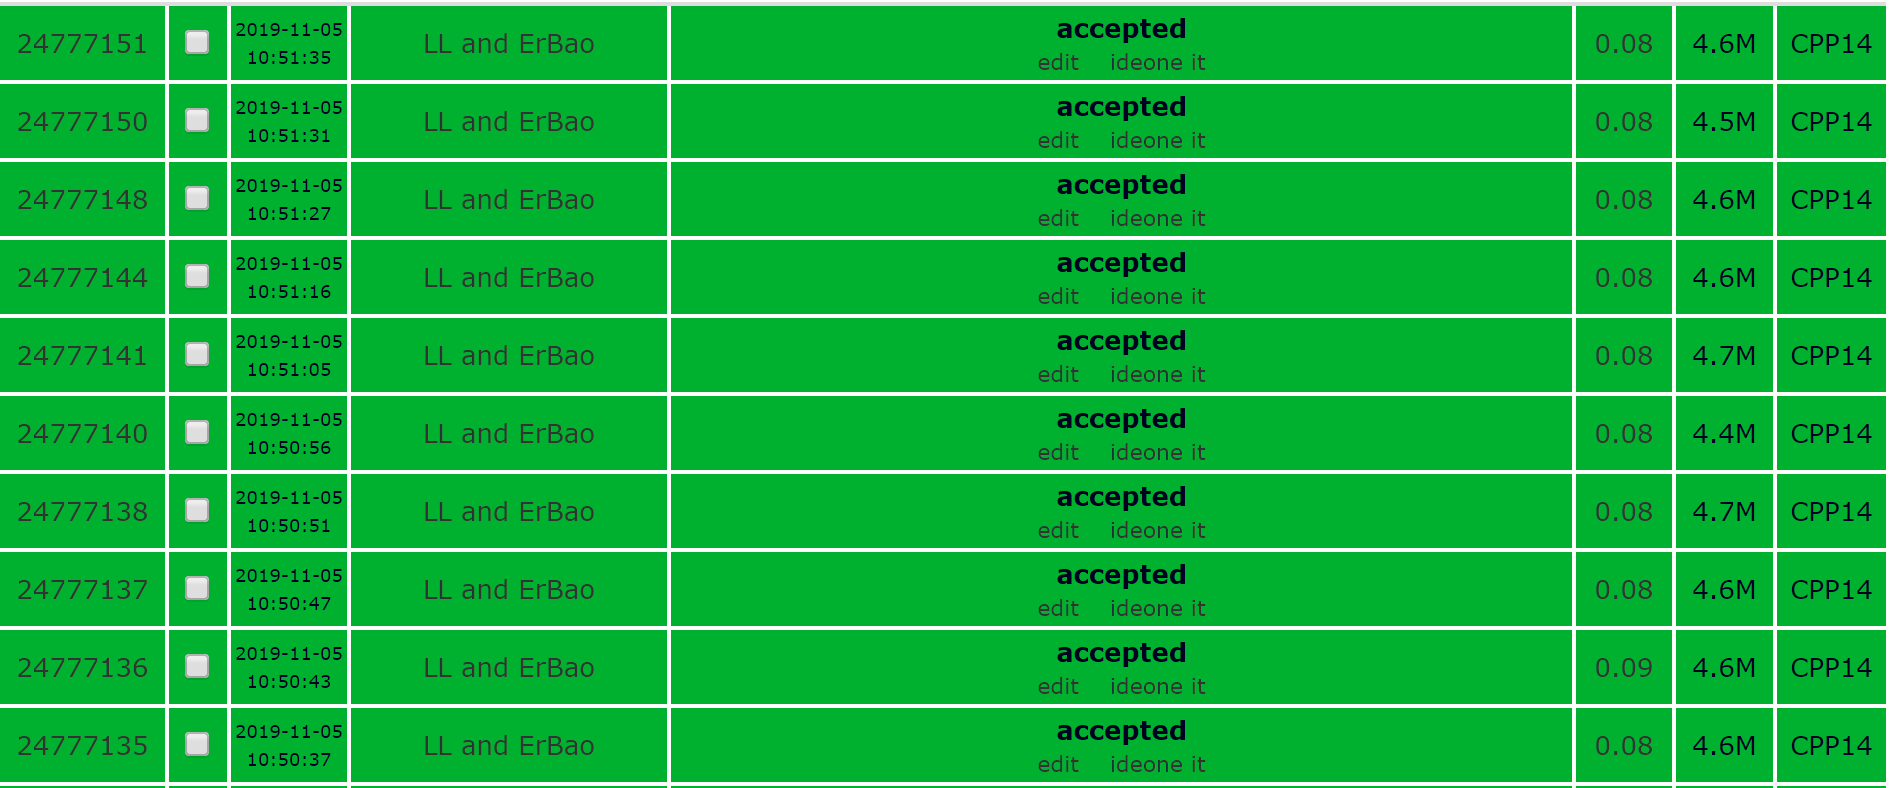
\includegraphics[width=\columnwidth]{bab5/img/hasil-pengumpulan-kode-program}
 \caption{Hasil Pengumpulan Kode Program Utama Dengan Algoritma reduksi polygon}
 \label{fig:hasil-pengumpulan-kode-program}
\end{figure}
		\chapter{BIODATA PENULIS}

\begin{wrapfigure}{l}{0.3\textwidth}
	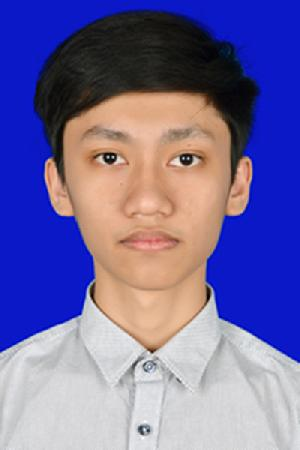
\includegraphics[height=0.3\textheight]{penutup/img/foto.jpeg}
\end{wrapfigure}

Penulis bernama Michael Julian Albertus, putra kedua dari tiga bersaudara yang lahir pada tanggal 2 Juli 1998 di Pekanbaru. Penulis telah mengenyam pendidikan di Sekolah Dasar Mardi Yuana Serang pada tahun 2004 hingga 2006, Sekolah Dasar Palm Kids pada tahun 2006 hingga 2009, Sekolah Dasar Negeri 005 Sukajadi Pekanbaru pada tahun 2009 hingga 2010, Sekolah Menengah Pertama Negeri 5 Pekanbaru pada tahun 2010 hingga 2013, dan Sekolah Menengah Atas Negeri 8 Pekanbaru pada tahun 2013 hingga 2015. Pada masa penulisan, penulis sedang menempuh masa studi S1 di Institut Teknologi Sepuluh Nopember, Surabaya di \jurusan.

Selama masa studi, penulis memiliki ketertarikan yang dalam mengenai \textit{artificial intelligence}, \textit{competitive programming}, dan rancang bangun aplikasi sistem informasi. Keinginan penulis dalam mengajar juga mendorong penulis menjadi asisten dosen pada mata kuliah Dasar Pemrograman, Struktur Data, dan Sistem Operasi. Karya penulis semasa perkuliahan diantaranya adalah pembangunan SheNeedsLab dan LPencerdas untuk acara Hackathon. Selama menempuh perkuliahan penulis juga aktif mengikuti kompetisi pemrograman tingkat nasional dan menjadi finalis pada lomba pemrograman COMPFEST (2017, 2018, dan 2019), INC Bina Nusantara (2017, 2018, dan 2019), FINDIT 2019, Arkavidia (2017,2018, dan 2019) dan menjadi Juara 3 HOLOGY 2018.

Di luar kesibukan akademik, penulis juga berkontribusi dalam berbagai kepanitiaan, baik dalam skala kecil (yaitu dalam kampus) maupun skala nasional. Kepanitian yang penulis ikuti adalah Schematics (2017 dan 2018). Kegiatan terakhir penulis adalah membantu kegiatan pelatihan nasional bagi peserta Olimpiade Komputer Indonesia pada Februari dan Maret 2019 lalu. Penulis dapat dihubungi melalui surel di michaeljulian98@gmail.com.


		
\end{sloppypar}
\end{document}